\documentclass[]{article}
\usepackage[margin = 1.5in]{geometry}
\setlength{\parindent}{0in}
\usepackage{amsfonts}
\usepackage{amssymb}
\usepackage{amsmath}
\usepackage{amsthm}
\usepackage{mathtools}
\usepackage{tikz}
\usepackage{qtree}
\usepackage{tikz-qtree}
\usepackage{float}
\usepackage[lined]{algorithm2e}
\usepackage[T1]{fontenc}
\usepackage{ae,aecompl}
\usepackage{color}
\usepackage{bussproofs}
\usepackage{enumerate}
\usepackage[pdftex,
  pdfauthor={Chris Thomson},
  pdftitle={CS 360: Introduction to the Theory of Computing},
  pdfsubject={Lecture notes from CS 360 at the University of Waterloo},
  pdfkeywords={CS 360, course notes, notes, Waterloo, University of Waterloo, theory, finite automata},
  pdfproducer={LaTeX},
  pdfcreator={pdflatex}]{hyperref}

\usepackage{cleveref}

\DeclarePairedDelimiter{\set}{\lbrace}{\rbrace}

\definecolor{darkish-blue}{RGB}{25,103,185}

\hypersetup{
    colorlinks,
    citecolor=darkish-blue,
    filecolor=darkish-blue,
    linkcolor=darkish-blue,
    urlcolor=darkish-blue
}

\theoremstyle{definition}
\newtheorem*{defn}{Definition}
\newtheorem*{theorem}{Theorem}
\newtheorem*{thesis}{Thesis}
\newtheorem*{lemma}{Lemma}
\newtheorem*{corollary}{Corollary}
\newtheorem*{aside}{Aside}
\newtheorem{ex}{Example}[section]

\crefname{ex}{Example}{Examples}

\setlength{\marginparwidth}{1.5in}
\newcommand{\lecture}[1]{\marginpar{{\footnotesize $\leftarrow$ \underline{#1}}}}

\makeatletter
\def\blfootnote{\gdef\@thefnmark{}\@footnotetext}
\makeatother

\begin{document}
	\let\ref\Cref

	\title{\bf{CS 360: Introduction to the Theory of Computing}}
	\author{Professor Shai Ben-David \\ \\ Fall 2013, University of Waterloo}
  \date{Notes taken by Chris Thomson}

  \blfootnote{I'd love to hear your feedback. Feel free to email me at \href{mailto:chris@cthomson.ca}{chris@cthomson.ca}.}

  \blfootnote{See \href{http://cthomson.ca/notes}{cthomson.ca/notes} for updates.
    \ifdefined\sha % Also, \commitDateTime should be defined.
    Last modified: \commitDateTime{} ({\href{https://github.com/christhomson/lecture-notes/commit/\sha}{\sha}}).
    \fi
  }

  \maketitle
  \newpage
  \tableofcontents
  \newpage

	\section{Introduction \& Course Structure} \lecture{September 10, 2013}
    \subsection{Course Structure}
      The grading scheme is 30\% assignments, 30\% midterm, and 40\% final. If your final grade is better than your midterm grade, your final will be worth 70\% and the midterm will be worth 0\%.
      \\ \\
      In terms of textbooks, any textbook relating to ``automata theory'', ``theory of computation'', or ``formal language theory'' is acceptable.
      \\ \\
      The professor's office is in DC 1311, and his office hours are on Tuesdays from 2:00 to 3:00 pm.
      \\ \\
      This course is mathematical. Consequently, relevant background courses are mainly mathematical (mostly logic) and  (almost) no programming.

    \subsection{Introduction}
      The goal of the course is to develop the theory of computation. We want to understand the mathematics that govern computers. We will explore questions like:
      \begin{itemize}
        \item What are computers?
        \item Which tasks can computers carry out?
        \item Which tasks are easy or hard for computers?
      \end{itemize}

      We make abstractions and use them as common properties that are relevant to many phenomenon. We aren't going to be focusing on any particular programming language or machine architecture, but instead, we'll focus on issues that underlie any automated computation.
      \\ \\
      These abstractions allow us to form conclusions that are relevant to computing in general, and not just for today's hardware and software.
      \\ \\
      This course has two key goals:
      \begin{enumerate}
        \item To familiarize you with the fundamentals of computer science theory.
        \item To develop the ability to reason formally and abstractly about computing.
      \end{enumerate}

    Throughout the course, we will follow two main threads concurrently: abstract models of computers, and computing tasks. We'll progress from simple models and simple tasks to complex models and complex tasks, and along the way connections will be made between the two.

    \subsection{Computing Tasks}
      We're going to focus on \textbf{decision problems}. Decisions problems are problems which have an input and produce a binary (yes/no) output. Some examples of decision problems are:
      \begin{itemize}
        \item Input: a number. Decision: is it a prime number?
        \item Input: email message. Decision: is it spam?
        \item Input: a graph. Decision: is it connected?
      \end{itemize}

      We're interested in seeing which of these questions a computer can carry out and how difficult are such tasks.

      \subsubsection{Modeling Decision Problems}
        We model decision problems using \textbf{formal languages}. A decision problem has two components:
        \begin{itemize}
          \item A domain set $X$.
          \item A language $L \subseteq X$.
        \end{itemize}

        Our decision problem is then ``for some $x \in X$, is $x \in L$?'' Re-examining our examples from earlier, we would define:
        \begin{itemize}
          \item $X = \mathbb{Z}$ (the set of all integers), and $L = $ the set of all prime numbers.
          \item $X = $ the set of all email messages, and $L = $ the set of all spam email messages.
          \item $X = $ the set of all graphs, and $L = $ the set of all connected graphs.
        \end{itemize}

        For further concreteness, we will fix some finite set $\Sigma$, which we will call the \textbf{alphabet}. Some examples of alphabets are $\set{a, b}$, $\set{0, 1}$, and $\set{0, 1, 2, 3}$.
        \\ \\
        $\Sigma^\star$ represents the set of all finite strings over the alphabet $\Sigma$. In many cases, we define $X = \Sigma^\star$. For example, if $\Sigma = \set{0, 1}$ then $\Sigma^\star = \set{ \epsilon, 0, 1, 00, 11, 01, 10, \ldots }$. Note that $\Sigma^\star$ is an infinite set, but every member of $\Sigma^\star$ is finite.
        \\ \\
        For the time being, we will define just one operation for strings: \textbf{concatenation}. Given two strings, $\sigma$ and $\eta$, we get $\sigma \eta$. That is,
          \AxiomC{$\sigma$}
          \AxiomC{$\eta$}
          \BinaryInfC{$\sigma \eta$}
          \DisplayProof . For example, if $\sigma = 01$ and $\eta = 111$, then $\sigma \eta$ is 01111.
        \\ \\
        \textbf{Languages} are subsets of $\Sigma^\star$ (that is, a language is a collection of strings). Some examples of languages include:
        \begin{itemize}
          \item $L = \emptyset$. This is the \textbf{empty language}, which no strings belong to. Note that $|L| = 0$. This is analogous to an empty fridge.
          \item $L = \set{ \epsilon }$. This is a non-empty language that contains one element ($|L| = 1$), which just happens to be $\epsilon$. This is analogous to having a fridge that contains only an empty pop can.
          \item $L = \set{\epsilon, 0, 01, 11111}$.
          \item $L = \Sigma^\star$.
        \end{itemize}

        A compiler's task of checking their input (the code of a program) to see if the program is valid (if the code is in the language), can be readily seen as checking membership in such a language (namely, the language of all binary sequences that represent valid code in the given programming language).

  \section{Inductive Definition of Sets and Structural Induction}
    We'll start off by reviewing some basic notions that were covered on CS 245, to ensure that everyone's on the same page.
      \subsection{Formal Tools for Defining Sets}
        We want languages to model every computational task, some of which are complex. We need several different methods for formally defining sets, since all languages are sets.

        \begin{enumerate}
          \item \textbf{List all members of the set}. This method is precise and concrete, but it makes look-ups difficult ($O(n)$) and it fails if the set is infinitely large.
          \item \textbf{Common property that characterizes the members of the set}. For example, consider the set of all even numbers. This set is not definable by a list because it's an infinite set. However, there is a common property that's shared between all members of the set: if you divide by two and examine the remainder, every member in the set will have a remainder of zero and only members of the set have this property.
          \item \textbf{Inductive definitions}. Methods (1) and (2) don't offer us a way to define a set of all your blood relatives, since there's no common property that characterizes that set. Instead, we could use \emph{inductive definitions}.
          \\ \\
          Inductive definitions of sets requires three components:
          \begin{itemize}
            \item A domain set $X$ (sometimes omitted if it is obvious).
            \item A core set $A$ (as in ``atoms''), such as $\set{ \text{me} }$.
            \item A set of operations $P$, such as $\set{ \text{``son of''}, \text{``father of''}, \text{``mother of''}}$. This set is a set of functions from $X \to X$.
          \end{itemize}

          Given these components, we define the \textbf{inductive set} $I(A, P)$ (say, the set of blood relatives), as all domain elements that can be reached from the core set by applying a finite sequence of operations from $P$.

          \begin{defn}
            $I(A, P)$ -- the \textbf{inductive set} defined by core $A$ and operations $P$ -- is the smallest set satisfying:
            \begin{itemize}
              \item Contains all members of $A$, and
              \item Closed under the operations in $P$.
            \end{itemize}
          \end{defn}

          \noindent \textbf{Examples:}
          \begin{itemize}
          \item Let the domain be the set of all real numbers ($\mathbb{R}$), the core set be $\set{2}$, and the set of operations be $\set{ \text{``add 2''}, \text{``subtract 2''}}$. The defined set is the set of all even numbers, both positive and negative.

          \item To define the set of all algebraic expressions, our core set would be $\set{x, y, z, 1, 2, 3, \ldots, a, b, c, \ldots}$, and our operations would be:
          \AxiomC{$\sigma$} \AxiomC{$\eta$} \BinaryInfC{$(\sigma + \eta)$} \DisplayProof,\AxiomC{$\sigma$} \AxiomC{$\eta$} \BinaryInfC{$(\sigma \cdot \eta)$} \DisplayProof.
          \end{itemize}
          Given a set (language) defined inductively, how can we tell if some $x \in X$ is in the language or not?

          \begin{ex}
            Let $X = \set{a, b}^\star$, $A = \set{a}$, and $P = $ \bigg\{ \AxiomC{X} \UnaryInfC{aX} \DisplayProof, \AxiomC{X} \UnaryInfC{Xa} \DisplayProof, \AxiomC{X} \AxiomC{Y} \BinaryInfC{bXY} \DisplayProof, \AxiomC{X} \AxiomC{Y} \BinaryInfC{XbY} \DisplayProof, \AxiomC{X} \AxiomC{Y} \BinaryInfC{XYb} \DisplayProof \bigg\}.
            \\ \\
            A typical question would be: is $abbaa \stackrel{?}{\in} I(A, P)$? The answer: yes! However, we must show how to generate $abbaa$ from $a$, using the operations in $P$, in a finite number of steps.

            \begin{enumerate}[1.]
            \item $a$, belongs to the core $A$.
            \item $baa$, after applying $P_3(a, a)$.
            \item $abbaa$, after applying $P_4(a, baa)$.
            \end{enumerate}

            Note that the first step must always be an element in the core set.
            \\ \\
            Is $\epsilon \in I(A, P)$? No. We could use simple reasoning to show that $\epsilon \not \in I(A, P)$ (each function in $P$ increases the length). However, in general, it is more difficult to prove non-membership of an element than it is to prove membership of another element.
          \end{ex}

          \begin{defn}
            A \textbf{certificate} (or \textbf{generating sequence}) for $x$ is a sequence of elements of $X, \theta_1, \theta_2, \theta_3, \ldots, \theta_n$ such that:
            \begin{itemize}
              \item $\theta_n = x$, and
              \item Every $\theta_i$ in the sequence is either an element of the core set $A$ or is the result of applying an operation from $P$ to a $\theta_j, \theta_l$ that appeared earlier in the sequence ($j < i$ and $l < i$). \lecture{September 12, 2013}
            \end{itemize}
          \end{defn}
        \end{enumerate}

        Our definition of $I(A, P)$ is still somewhat informal, however. We haven't formally defined what it means for a subset to be the \emph{smallest} subset, and we also haven't formally defined what it means for a set to be ``closed'' under a set of operations.

        \subsection{More on Inductive Sets and Structural Induction}
        We say that a set $B$ is \textbf{closed under the operations of $\boldsymbol P$} if for every $f \in P$ and every $x, y \in B$, $f(x, y) \in B$ (for concreteness, we considered here an $f$ that accepts two inputs, but it may also be a unary function, $f(x)$ or ternary $f(x,y, z)$, etc.). For example, the set of even numbers is closed under the operation +.
        \\ \\
        Now, let's redefine $I(A, P)$ in a more formal way:
        $$
          I(A, P) = \bigcap \left\{ B : A \subseteq B ~\text{ and } ~B ~\text{ is closed under } ~P \right\}
        $$

        Note that $I(A, P)$ is the intersection over the \emph{entire} collection of sets (and is therefore uniquely defined).

        \begin{ex}
          Let $X = \mathbb{N}, A = \set{10}, P = \set{+}$.
          \\ \\
          $I(A, P)$ is defined as the intersection of all sets $B$ such that $ A \subseteq B $ and $B$ is closed under $P$ (that is, $B$ is closed under $+$). So, we have:
          \begin{itemize}
            \item $B_1 = \set{\text{all even numbers}}$
            \item $B_2 = \set{\text{all numbers divisible by 5}}$
            \item $B_3 = \set{\text{all numbers divisible by 10}}$
          \end{itemize}

          In this case, $I(A, P) = \set{10, 20, 30, \ldots}$, since $I(A, P)$ must be the minimal set among all possible sets $B$ (or, in other words, the multiples of 10 are exactly the numbers that belong to each and every of these sets $B$).
        \end{ex}

        \begin{aside}
          \begin{align*}
            \bigcap \left\{ [0, r] : r > 0 \right\} &= \set{0} \\
            \bigcap \left\{ (0, r) : r > 0 \right\} &= \emptyset \\
            \bigcup \left\{ \set{1, \ldots, n} : n \in \mathbb{N} \right\} &= \mathbb{N} \\
            \bigcap \left\{ \set{1, \ldots, n} : n \in \mathbb{N} \right\} &= \set{1}
          \end{align*}
        \end{aside}

        The equivalence of the two definitions of $I(A, P)$ is not immediately clear. We claim that $I(A, P)$ is closed under the operations of $P$, and $A \subseteq I(A, P)$.

        \begin{proof}
          Pick any $x, y \in I(A, P)$ and operation $f \in P$. For every $B$ which contains $A$ and is closed under $P$, $x, y \in B$ (since $I(A,P)$ is the intersection of all such $B$'s).
          \\ \\
          Since every such $B$ is closed under $P$, $f(x, y) \in B$ for every such $B$. Therefore, $f(x, y) \in \cap \set{ B : A \subseteq B \text{ and } B \text{ is closed under } P}$, so $f(x,y) \in I(A, P)$.
          \\ \\
          \underline{Exercise}: prove that $A \subseteq I(A, P)$.
        \end{proof}

        \begin{corollary}[Proof by Structural Induction Theory]
          Any $B \subseteq X$ which contains $A$ and is closed under $P$ is a superset of $I(A, P)$. Namely, $I(A, P) \subseteq B$.
        \end{corollary}

        We could rephrase this corollary as follows: given any set $B$, if you want to prove that $I(A, P) \subseteq B$, it suffices to show:
        \begin{itemize}
          \item $A \subseteq B$, and
          \item $B$ is closed under $P$.
        \end{itemize}

      \subsubsection{Proof by Structural Induction}
        Let's say we want to show that for every $n$, $n^2 + n$ is even. A proof by usual (mathematical) induction requires us to show two things:
        \begin{itemize}
          \item Prove the claim holds for $n = 1$. This is equivalent to showing that $A \subseteq B$.
          \item Prove that if the claim holds for $n$, it also holds for $n + 1$. This is equivalent to showing that $B$ is closed under $P$.
        \end{itemize}

        How is this the same as structural induction? Usual induction shows that $\mathbb{N} = I(A, P)$, where $A = \set{1}$ and $P = \set{ \text{``+1''}}$. That is, mathematical induction is just one specific case of structural induction.

      \subsection{Examples of Proofs by Structural Induction}
        \begin{ex}
          Imagine we have three paper cups placed on a desk, with two of them facing upwards and one upside down. You must flip exactly two cups at a time. We want to get all of the cups facing upwards. Can we prove that this goal is not achievable?
          \\ \\
          Let $X$ be the set of all possible configurations of the cups. Let our core set $A$ contain only the state ``[up] [down] [up]''. Let our set of operations $P$ contain:
          \begin{itemize}
            \item $P_1$: flip the two rightmost cups.
            \item $P_2$: flip the two leftmost cups.
            \item $P_3$: flip the rightmost and leftmost cups.
          \end{itemize}

          We claim that the state ``[up] [up] [up]'' $\not \in I(A, P)$.
          \begin{proof}
            Let $B$ be the set of all configurations with an even number of ``up'' cups.
            \\ \\
            We want to show that $I(A, P) \subseteq B$. This would show that ``[up] [up] [up]'' is not attainable because it is not a member of $B$. We will use structural induction to show this.
            \\ \\
            \textbf{Induction base}: $A \subseteq B$.
            \\ \\
            \textbf{Induction step}: $B$ is closed under $P$. Namely, if $c \in B$, then $P_1(c), P_2(c)$, and $P_3(c) \in B$. There are three cases:
            \begin{itemize}
              \item We flip one ``up'' cup and one ``down'' cup. This is a difference of +0 ``up'' cups.
              \item We flip two ``up'' cups. This causes us to remove two (which is even) from an already even number, which gives us another even number of ``up'' cups.
              \item We flip two ``down'' cups. This causes us to add two (which is even) to an already even number, which gives us another even number of ``up'' cups.
            \end{itemize}

            Note that these three cases show us that no matter which operation we use, it is not possible to obtain all three ``up'' cups, since the number of ``up'' cups will always be even.
          \end{proof}
        \end{ex}

        \begin{ex}
          Earlier, we defined $X = \set{a, b}^\star$, $A = \set{a}$, and $P = $ \bigg\{ \AxiomC{X} \UnaryInfC{aX} \DisplayProof, \AxiomC{X} \UnaryInfC{Xa} \DisplayProof, \AxiomC{X} \AxiomC{Y} \BinaryInfC{bXY} \DisplayProof, \AxiomC{X} \AxiomC{Y} \BinaryInfC{XbY} \DisplayProof, \AxiomC{X} \AxiomC{Y} \BinaryInfC{XYb} \DisplayProof \bigg\}.
          \\ \\
          For this example, let $\#_a(x)$ denote the number of ``a''s in the string $x$ and similarly, let $\#_b(x)$ denote the number of ``b''s in the string $x$.
          \\ \\
          \textbf{Claim}: every member of $I(A, P)$ has more ``a''s than ``b''s. To put this more simply, let $B = \set{ x : \#_a(x) > \#_b(x) }$. We wish to show that $I(A, P) \subseteq B$.
          \begin{proof}
            We will prove this claim by structural induction.
            \\ \\
            \textbf{Induction base}: $A \subseteq B$. It is trivial to see that the string ``a'' has more ``a''s than ``b''s (since it has no ``b''s).
            \\ \\
            \textbf{Induction step}: if $x, y \in B$, then we must show that $P_1(x) \in B, P_2(x) \in B, P_3(x, y) \in B, P_4(x,y) \in B$, and $P_5(x, y) \in B$.
            \\ \\
            It is clear that for $P_1$ and $P_2$, one ``a'' is being added to a string that must already include more ``a''s than ``b''s, so this trivially holds true.
            \\ \\
            The case of $P_3$ isn't as immediately obvious. Assume $\#_a(x) > \#_b(x)$, and $\#_a(y) > \#_b(y)$. So, $\#_a(x) \ge \#_b(x) + 1$ and $\#_a(y) \ge \#_b(y) + 1$. This gives us $\#_a(xy) \ge \#_b(xy) + 2$.
            \\ \\
            Now, note that $\#_a(bxy) = \#_a(xy)$, and $\#_b(bxy) = \#_b(xy) + 1$. We can conclude that $\#_a(bxy) \ge \#_b(bxy) + 1 > \#_b(bxy)$.
            \\ \\
            A similar argument applies for $P_4$ and $P_5$.
          \end{proof}
        \end{ex}

      \subsection{Regular Languages}
        For us, tasks will always be decision problems. That is, given $L \subseteq \set{a, b}^\star$ and input $x \in \set{a, b}^\star$, decide if $x \in L$.
        \\ \\
        The set of all possible tasks is $\set{L : L \subseteq \set{a, b}^\star}$. This set is an infinite set of finite strings.
        \\ \\
        Recall that not all infinite sets have the same size. The set of all finite strings $\set{a, b}^\star$ is a ``small'' infinite set, meaning it is \textbf{countable}. However, the set of all subsets of $\set{a, b}^\star$ is a ``large'' infinite set, which is \textbf{uncountable}.
        \\ \\
        The set of all possible computer programs is a subset of $\set{0, 1}^\star$. Note that since every program is a \emph{finite} string, the set of all possible programs is countable.
        \\ \\
        In summary, we have an uncountable number of tasks, but a countable number of programs (and each program is suitable for carrying out at most a single task). This implies that there are tasks (languages) for which no program exists (namely, for such languages, $L$, there exists no program that will figure out correctly for every string $x$ whether it is a member of $L$ or not).

      \subsection{Defining Interesting Families of Tasks} \lecture{September 17, 2013}
        \begin{defn}
          The \textbf{empty string} can be denoted as either $\epsilon$ or $\lambda$.
        \end{defn}

        \subsubsection{Operations on Languages}
          There are several operations that we can perform on languages.
          \\ \\
          We can use \textbf{standard set operations}, including $\bigcup, \bigcap$, complement ($\overline A$), and set difference ($A \textbackslash B$). You should be familiar with how these standard operations are defined.
          \\ \\
          Since we focus on subsets of the set of finite strings, $\Sigma^\star$, we can also use \textbf{operations on sets of such strings}. Let's go into more detail of how these string set operations are defined.

          \begin{enumerate}
            \item \textbf{The concatenation operation}. Given $L_1, L_2 \subseteq \Sigma^\star$, we define $L_1 L_2 = \set{ w_1 w_2 : w_1 \in L_1, w_2 \in L_2 }$.

            \begin{ex}
            Let $L_1 = \set{0, 011}$ and $L_2 = \set{ \epsilon, 110 }$. Then $L_1 L_2 = \set{0, 0110, 011, 011110 }$.
            \end{ex}

            Concatenation is not always commutative. Consider $L_1 = \set{0}$ and $L_2 = \set{1}$. We have $L_1 L_2 = \set{01}$ but $L_2 L_1 = \set{10}$, so $L_1 L_2 \ne L_2 L_1$.
            \\ \\
            Can $L_1 \subseteq L_1 L_2$? Yes, but only if $\epsilon \in L_2$. Otherwise, $L_1 \not \subseteq L_1 L_2$.

            \item \textbf{The power operation}. Given any language $L$, define:
              \begin{itemize}
                \item $L^0 = \set{ \epsilon }$
                \item $L^{n + 1} = L^n L$ for every $n > 0$
              \end{itemize}

              In particular, note that $L^1 = \set{ \epsilon} L = L$.

              \begin{ex}
                Let $L = \set{ 0, 1 }$. Then $L^n$ is the set of all ($\set{0, 1}$) strings.
              \end{ex}

            \item \textbf{The star (Kleene) operation}. For any language $L$, $L^\star = \displaystyle \bigcup_n L^n$. That is, $L^\star$ is the set of all finite concatenations of strings from $L$. Note that $L^\star$ includes $L^0$, which means $\epsilon \in L^\star$.
          \end{enumerate}

          \noindent \textbf{Examples:}
            \begin{itemize}
              \item $\set{1}^\star$ is the set of all finite strings of 1s.
              \item $\set{0, 1}^\star$ is the set of all finite $\set{0, 1}$ strings.
              \item Can $L^\star = L$? Yes. Consider $L = \set{ \epsilon }$, or $(L^\star)^\star = L^\star$ for any $L$.
              \item Can $L^\star$ be finite? Yes. Consider $L = \set{ \epsilon }$ or $L = \emptyset$.
            \end{itemize}

        \subsubsection{The Set of Regular Languages}
          Given some finite alphabet set $\Sigma$, let $X = \Sigma^\star$. We will also define our core set to be:
          $$
            A = \set{\emptyset, \set{\epsilon}} \cup \set{ \set{a} : a \in \Sigma }
          $$

          For instance, suppose $\Sigma = \set{0, 1}$. Then $A = \set{ \emptyset, \set{ \epsilon }, \set{ 0 }, \set{ 1 } }$. Next, we'll define our set of operations $P$:
          $$
            P = \text{ \bigg\{ \AxiomC{$L_1$} \AxiomC{$L_2$} \BinaryInfC{$L_1 \cup L_2$} \DisplayProof, \AxiomC{$L_1$} \AxiomC{$L_2$} \BinaryInfC{$L_1 \cdot L_2$} \DisplayProof, \AxiomC{$L$} \UnaryInfC{$L^\star$} \DisplayProof \bigg\}}
          $$

          A language is said to be \textbf{regular} if it belongs to $I(A, P)$, for this $A$ and $P$.
          \\ \\
          To prove a language is regular, you must be able to show how to generate it.

          \begin{ex}
            $\set{0, 1, 01}$ is regular.
            \begin{proof}
              \begin{align}
                \set{0} &\text{ core} \\
                \set{1} &\text{ core} \\
                \set{01} &\text{ product} \\
                \set{0, 1} &\text{ union of (1) and (2)} \\
                \set{0, 1, 01} &\text{ union of (3) and (4)}
              \end{align}
              \setcounter{equation}{0}
            \end{proof}
          \end{ex}

          \textbf{Claim 1}: for every (finite) string $\sigma$, $\set{\sigma}$ is a regular language. It's easy to see this is true, because you can generate the language by concatenating the languages that represent individual letters.
          \\ \\
          \textbf{Claim 2}: every finite language is regular. Since we know every $\set{\sigma}$ is regular, so is any finite unions of such languages.

          \begin{ex}
            Let $L_\text{even}$ be the language of all words of even length. $L_\text{even}$ is regular. We can form every word in $L_\text{even}$ using the expression $(\set{0, 1} \set{0, 1})^\star$.
          \end{ex}

          \begin{ex}
            Let $L_\text{equal} = \set{ w : \#_0(w) = \#_1(w) }$. $L_\text{equal}$ is not regular. We can't prove this yet though.
          \end{ex}

      \subsection{Explicit Descriptions of Regular Languages: Regular Expressions}
        A \textbf{regular expression} is just a word in a language that is designed to describe languages.

        \subsubsection{Defining The Set of Regular Expressions}
          Given some alphabet $\Sigma$, let $X$ be defined as
          $$
            X = (\Sigma \cup \set{+, \star, (, ), \emptyset, \epsilon})^\star
          $$

          We will define our core set $A$ as
          $$
            A = \set{\emptyset, \epsilon} \cup \set{ a : a \in \Sigma }
          $$

          Finally, we will define our set of operations $P$ as
          $$
            P = \left\{ \text{\AxiomC{$r_1$} \AxiomC{$r_2$} \BinaryInfC{$r_1 + r_2$} \DisplayProof, \AxiomC{$r_1$} \AxiomC{$r_2$} \BinaryInfC{$r_1 r_2$} \DisplayProof, \AxiomC{$r$} \UnaryInfC{$r^\star$} \DisplayProof, \AxiomC{$r$} \UnaryInfC{$(r)$} \DisplayProof } \right\}
          $$

          A regular expression is any member of this $I(A, P)$.
          \\ \\
          Suppose $\Sigma = \set{a, b}$. Some regular expressions over $\Sigma$ are $a$, $ab$, $a + b$, $a(a + \epsilon)^\star$, and $(a + b)(a + b)$.
          \\ \\
          \textbf{Claim}: in any regular expression, the number of $+$ symbols is at least one less than the number of symbols from the set $\Sigma \cup \set{ \epsilon, \emptyset }$. The proof of this (by structural induction) is left as an exercise.

        \subsubsection{Mapping Regular Expressions to Languages}
          We will define a mapping $L$ such that $L: \text{Regular Expression} \to \text{Language}$. We define such a mapping $L$ recursively over the definition of regular expressions.

          \begin{itemize}
            \item $L(\epsilon) = \set{ \epsilon }$
            \item $L(a) = \set{ a }$ for every $a \in \Sigma$
          \end{itemize}

          Assume $L(r_1)$ and $L(r_2)$ are already defined. We then define the mappings for each operation:
          \begin{itemize}
            \item $L(r_1 r_2) = L(r_1) L(r_2)$
            \item $L(r_1 + r_2) = L(r_1) \cup L(r_2)$
            \item $L(r_1^\star) = (L(r_1))^\star$
            \item $L((r_1)) = L(r_1)$
          \end{itemize}

          \noindent \textbf{Examples}:
          \begin{itemize}
            \item Let $r = (0 + 1)$. Then $L(r) = \set{0, 1}$.
            \item Let $r = 01$. Then $L(r) = \set{01}$.
            \item Let $r = (01)^\star$. Then $L(r) = \set{ \epsilon, 01, 010101, 01\ldots0101\ldots01, \ldots}$.
            \item Let $r = (01)^\star + (10)^\star$. Then $L(r)$ is the set of all alternating strings that either start with 0 and end with 1, or start with 1 and end with 0.
          \end{itemize}

          Find an expression $r$ such that $L(r)$ is the set of \emph{all} alternating strings. One such expression is $r = (0 + \epsilon)(10)^\star(1 + \epsilon)$. Another expression to represent the same language is $r' = (01)^\star + (10)^\star + 1(01)^\star + 0(10)^\star$.
          \\ \\
          Since $L(r) = L(r')$ represent the same language, this shows that there is no \emph{unique} regular expression to describe a language. Multiple distinct regular expressions can represent the same language.

        \subsubsection{Uses of Regular Expressions}
          Regular expressions are often useful to search for patterns in code. For example, if you were looking for all strings that start with ``a'' and end with ``b'', you could use the regular expression $a(a + b)^\star b$.
          \\ \\
          Regular expressions are also used in compilers. Compilers need to find certain patterns in the code they're given to compile, in order to perform the parsing step of the compilation.
          \\ \lecture{September 19, 2013} \\
        \emph{The lecture from September 19, 2013 is omitted. If you have notes from this lecture, feel free to email me (\href{mailto:chris@cthomson.ca}{chris@cthomson.ca}) and I'll include them here.}

  \section{Computing Machines} \lecture{September 24, 2013}
    \subsection{Deterministic Finite Automata}
      The first model of computing machines that we'll discuss are \textbf{deterministic finite automata} (also known as \text{DFA}s). A DFA is denoted by $A = (\Sigma, Q, q_0, \delta, F)$, where
      \begin{itemize}
        \item $\Sigma$ is the alphabet (the set of letters) of the DFA.
        \item $Q$ is the set of all states in the DFA.
        \item $q_0$ is the initial state.
        \item $\delta$ is the transition function.
        \item $F$ is the set of accepting states. (Note that there can be more than one accepting state.)
      \end{itemize}

      Every DFA can be represented with a bubble diagram, to make it easier to visualize.
      \begin{ex}
        A bubble diagram that represents the DFA that accepts all strings with an even number of $0$s and an odd number of $1$s is as follows:

        % http://madebyevan.com/fsm/ is a great tool for generating these.
        % It generates somewhat verbose code, unfortunately.
        \begin{center}
          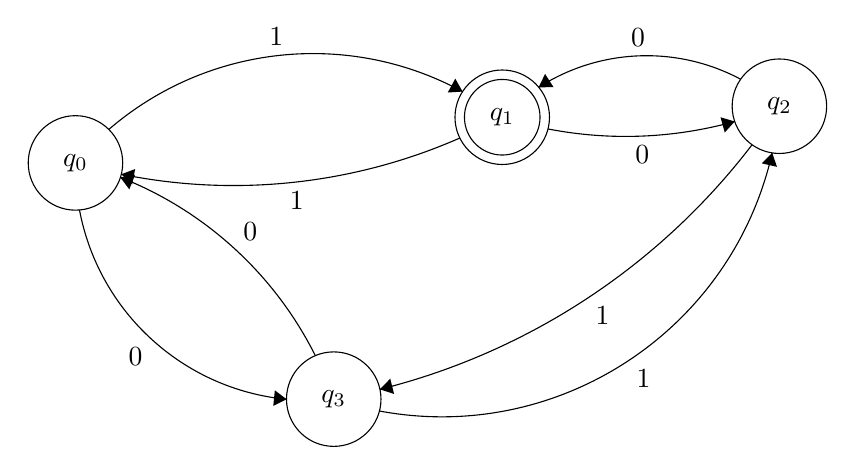
\begin{tikzpicture}[scale=0.2]
          \tikzstyle{every node}+=[inner sep=0pt]
          \draw [black] (11.1,-17.2) circle (3);
          \draw (11.1,-17.2) node {$q_0$};
          \draw [black] (38.2,-14.3) circle (3);
          \draw (38.2,-14.3) node {$q_1$};
          \draw [black] (38.2,-14.3) circle (2.4);
          \draw [black] (55.8,-13.6) circle (3);
          \draw (55.8,-13.6) node {$q_2$};
          \draw [black] (27.5,-32.2) circle (3);
          \draw (27.5,-32.2) node {$q_3$};
          \draw [black] (13.215,-15.077) arc (130.7768:61.43928:19.862);
          \fill [black] (35.68,-12.67) -- (35.22,-11.85) -- (34.74,-12.73);
          \draw (23.86,-9.78) node [above] {$1$};
          \draw [black] (35.507,-15.62) arc (-66.28802:-101.4959:35.741);
          \fill [black] (14.01,-17.92) -- (14.7,-18.57) -- (14.89,-17.59);
          \draw (25.15,-19.02) node [below] {$1$};
          \draw [black] (24.505,-32.212) arc (-95.55965:-169.33456:14.845);
          \fill [black] (24.51,-32.21) -- (23.76,-31.64) -- (23.66,-32.63);
          \draw (14.91,-28.88) node [below] {$0$};
          \draw [black] (52.963,-14.571) arc (-74.43247:-101.01232:25.813);
          \fill [black] (52.96,-14.57) -- (52.06,-14.3) -- (52.33,-15.27);
          \draw (47.09,-16.04) node [below] {$0$};
          \draw [black] (54.064,-16.046) arc (-37.38097:-75.98969:42.768);
          \fill [black] (30.43,-31.58) -- (31.33,-31.87) -- (31.09,-30.9);
          \draw (44.57,-26.32) node [below] {$1$};
          \draw [black] (55.342,-16.562) arc (-12.78146:-100.5892:21.52);
          \fill [black] (55.34,-16.56) -- (54.68,-17.23) -- (55.65,-17.45);
          \draw (47.18,-30.28) node [below] {$1$};
          \draw [black] (40.512,-12.399) arc (122.65769:61.89753:12.697);
          \fill [black] (40.51,-12.4) -- (41.46,-12.39) -- (40.92,-11.55);
          \draw (46.83,-9.86) node [above] {$0$};
          \draw [black] (13.954,-18.118) arc (68.51255:26.59325:23.447);
          \fill [black] (13.95,-18.12) -- (14.52,-18.88) -- (14.88,-17.95);
          \draw (22.2,-22.15) node [above] {$0$};
          \end{tikzpicture}
        \end{center}
      \end{ex}

      To define $L(A)$, we extend $\delta: Q \times \Sigma \to Q$, to: $\hat{\delta}: Q \times \Sigma^\star \to Q$. Now, we define the language accepted by DFA $A$ as:
      $$
        L(A) = \set{ w : \hat{\delta}(q_0, w) \in F }
      $$

      \textbf{Claim}: For this automaton, $L(A) = \set{ w : \#_0(w) \text{ is even, and } \#_1(w) \text{ is odd}}$. But how do we prove this?
      \\ \\
      Let's rephrase our claim. For every $w \in \set{0, 1}^\star$, if $\#_0(w)$ is even and the $\#_1(w)$ is odd, then $A$ accepts $w$, and otherwise, $A$ does not accept $w$.
      \\ \\
      Since we said ``for every $w \in \set{0, 1}^\star$'', that should be a give away that we should use structural induction for this proof.
      \\ \\
      Let's define $\set{0, 1}^\star$ inductively. Note that we are \emph{not} yet defining the set of accepted members for the DFA, but instead, we are aiming to inductively define the set of all possible words across the alphabet $\Sigma = \set{0, 1}$.
      \\ \\
      We have our core set $A = \set{ \epsilon }$ (not to be confused with the $A$ we're using to denote the DFA). We also have two operations for any string $\sigma$,
      $$
        P = \bigg\{ \text{\AxiomC{$\sigma$} \UnaryInfC{$\sigma 1$} \DisplayProof, \AxiomC{$\sigma$} \UnaryInfC{$\sigma 0$} \DisplayProof} \bigg\}
      $$

      Rather than proving our claim directly, it will be easier to prove a stronger claim, which characterizes every state of the machine. This stronger claim (four claims, in fact) will be easier to prove because we'll have more to work with in our induction hypothesis.
      \\ \\
      For every $w \in \set{0, 1}^\star$:

      \begin{itemize}
        \item If $\#_0(w)$ is even and $\#_1(w)$ is even, then $\hat{\delta}(q_0, w) = q_0$.
        \item If $\#_0(w)$ is even and $\#_1(w)$ is odd, then $\hat{\delta}(q_0, w) = q_1$.
        \item If $\#_0(w)$ is odd and $\#_1(w)$ is odd, then $\hat{\delta}(q_0, w) = q_2$.
        \item If $\#_0(w)$ is odd and $\#_1(w)$ is even, then $\hat{\delta}(q_0, w) = q_3$.
      \end{itemize}

      \begin{proof}
        We will prove the four claims using structural induction on $\set{0, 1}^\star$.
        \\ \\
        \textbf{Base case}: $w = \epsilon$. It's easy to see that $\#_0(w)$ is even, $\#_1(w)$ is even, and indeed, $\hat{\delta}(q_0, \epsilon) = q_0$.
        \\ \\
        \textbf{Induction step}: assume the four claims hold for $w$. We need to show they hold for $w_0$ and $w_1$.
        \\ \\
        \underline{The operation $w_0$}: if $\#_0(w_0)$ is even and $\#_1(w_0)$ is even, then $\#_0(w)$ is odd and $\#_1(w)$ is even. By the induction hypothesis, $\hat{\delta}({q_0, w}) = q_3$.
        \\ \\
        By the definition of $\hat{\delta}$, $\hat{\delta}(q_0, w_0) = \delta( \hat{\delta}(q_0, w), 0) = \delta(q_3, 0) = q_0$.
        \\ \\
        In order to finish this proof, we still need to prove the other three cases for $w_0$ and all four cases for $w_1$.
      \end{proof}

      Every task carried out by a DFA $A$ has the general form: ``given some input string $w$, decide if $w \in L(A)$''. In particular, we can say each $A$ handles the decision problem of the language $L(A)$. DFAs perform this task by consuming one character of $w$ at a time.
      \\ \\
      Note that not every language can be represented by a DFA. The following languages can all be handled by a DFA:
      \begin{itemize}
        \item $\set{ \epsilon }$
        \item $\Sigma^\star$
        \item For every $a \in \Sigma, \set{a}$
        \item For every $w \in \Sigma^\star, \set{w}$
      \end{itemize}

      \subsubsection{Closure Operations}
        Is the family of languages that can be computed by a DFA closed under $\cup, \cap$, set difference, concatenation, $L^\star$, etc?
        \\ \\
        \textbf{Claim}: if each of $L_1, L_2$ can be computed by some DFA, then so can $L_1 \cap L_2, L_1 \cup L_2$, and $L_1 \backslash L_2$.

        \begin{proof}
          Let $A_1$ and $A_2$ be DFAs such that $L(A_1) = L_1$ and $L(A_2) = L_2$. Let's construct some DFA $A_3$ such that $L(A_3) = L_1 \cap L_2$.
          \\ \\
          The general idea is to run the two machines, $A_1$ and $A_2$, in parallel, and if $w \in F$ in both machines, accept $w$ for $L_1 \cap L_2$.
          \\ \\
          Given any two automata $A_1 = (\Sigma, Q_1, q_0^1, \delta_1, F_1)$ and $A_2 = (\Sigma, Q_2, q_0^2, \delta_2, F_2)$, we define the \textbf{product automaton} as
          $$
            A_1 \times A_2 = (\Sigma, Q_1 \times Q_2, (q_0^1, q_0^2), \delta_{A_1 \times A_2}, F_{A_1 \times A_2})
          $$
          where $\Sigma$ is the same alphabet as defined previously, $Q_1 \times Q_2 = \set{ (p, q) : p \in Q_1, q \in Q_2 }$, and $\delta_{A_1 \times A_2}((p, q), a) = (\delta_1(p, a), \delta_2(q, a))$.
          \\ \\
          $F$ will be defined differently depending on which combination of $L_1$ and $L_2$ we wish to compute. For example:
          \begin{itemize}
            \item $F_{A_1 \cap A_2} = \set{ (p, q) : p \in F_1 \text{ and } q \in F_2 }$
            \item $F_{A_1 \cup A_2} = \set{ (p, q) : p \in F_1 \text{ or } q \in F_2 }$
            \item $F_{A_1 \backslash A_2} = \set{ (p, q) : p \in F_1 \text{ and } q \not \in F_2 }$
          \end{itemize}

          \textbf{Conclusion}: if $L_1$ and $L_2$ both have DFAs, then so do $L_1 \cap L_2, L_1 \cup L_2, L_1 \backslash L_2, L_1 \Delta L_2$, etc. (any boolean operation on sets). However, note that the product automaton does not tell us if a language is closed under $L^\star$ or concatenation.
          \\ \\
          Is it true that whenever $L$ has a DFA, then so does its complement, $L^C = \Sigma^\star \backslash L$? Yes, its DFA is $A_{\Sigma^\star \times L}$. Let $A = (\Sigma, Q, q_0, \delta, F)$ be a DFA such that $L(A) = L$, then let $A^C = (\Sigma, Q, q_0, \delta, Q \backslash F)$. Then, $L(A^C) = L^C$.
          \\ \\
          Since in our definition of a DFA we required that for every state $q \in Q$ and every letter $a \in \Sigma$, $q$ has some outgoing edge labeled by $a$ (we are never stuck).
        \end{proof}

      \subsubsection{The Relationship Between Regular Expressions and DFAs} \lecture{September 26, 2013}
        \textbf{Claim}: for every regular expression $r$, there exists some DFA $A$ such that $L(r) = L(A)$.

        \begin{proof}
          We will prove this claim by structural induction on the set of regular expressions.
          \\ \\
          \textbf{Base case}: the elements of the core set of regular expressions are $\set{ \epsilon, \underbrace{a, b, \ldots}_{\Sigma}, \emptyset}$. For each of these, we should show that there exists some DFA $A$ such that $L(A) = L(r)$.
          \begin{itemize}
            \item $L(\epsilon) = \set{ \epsilon }$. We have seen such an $A$.
            \item $L(\emptyset) = \emptyset$. We have seen such an $A$.
            \item For every $a \in \Sigma, L(a) = \set{a}$ and there exists some DFA $A$ such that $L(A) = \set{a}$.
          \end{itemize}

          \textbf{Inductive step}: we must show that under each operation the claim continues to hold. Recall the operations we defined on regular expressions to be
          $$
            P = \bigg\{ \text{\AxiomC{$r_1$} \AxiomC{$r_2$} \BinaryInfC{$r_1 + r_2$} \DisplayProof, \AxiomC{$r_1$} \AxiomC{$r_2$} \BinaryInfC{$r_1 r_2$} \DisplayProof, \AxiomC{$r$} \UnaryInfC{$r^\star$} \DisplayProof, \AxiomC{$r$} \UnaryInfC{$(r)$} \DisplayProof} \bigg\}
          $$

          \begin{enumerate}
            \item \underline{Consider the + operation}. Assume there are automata $A_1, A_2$ such that $L(r_1) = L(A_1)$ and $L(r_2) = L(A_2)$. We need to show that there exists some $A_3$ such that $L(A_3) = L(r_1 + r_2)$.
            \\ \\
            Recall that $L(r_1 + r_2) = L(r_1) \cup L(r_2)$. We saw that given $A_1, A_2$ we can construct $A_3$ such that $L(A_3) = L(A_1) \cup L(A_2)$.

            \item \underline{Consider the concatenation operation}. Assume $L(A_1) = L(r_1)$ and $L(A_2) = L(r_2)$. We need to define $A_3$ such that $L(A_3) = L(r_1 r_2) = L(A_1) L(A_2)$. Note that
            $$
              L(A_1) L(A_2) = \set{ w w' : w \in L(A_1), w' \in L(A_2) }
            $$

            One idea on how to approach this is to take DFAs $A_1$ and $A_2$ and merge each final state in $A_1$ with the initial state of $A_2$ (and make the states no longer final states). However, this approach will not suffice because we could then have multiple edges for the same letter, leading out of those newly-merged states.
            \\ \\
            In order to solve this problem, we need to take a detour to define a new family of machines. We'll return to this proof at a later point in time. \qedhere
          \end{enumerate}
        \end{proof}

    \subsection{Non-deterministic Finite Automata (NFAs)}
      NFAs are similar to deterministic finite automata, except they allow more edges on a state than there are letters in $\Sigma$. You can create multiple paths to be followed simultaneously.
      \\ \\
      We define an NFA $N$ as $N = (\Sigma, Q, q_0, \delta, F)$ where $\Sigma, Q, q_0$, and $F$ are exactly the same as in DFAs. However, for NFAs, we define $\Sigma: Q \times \Sigma \to \set{ B : B \subseteq Q }$.

      \begin{ex}
        Will this machine (an NFA) accept $a$?
        \begin{center}
          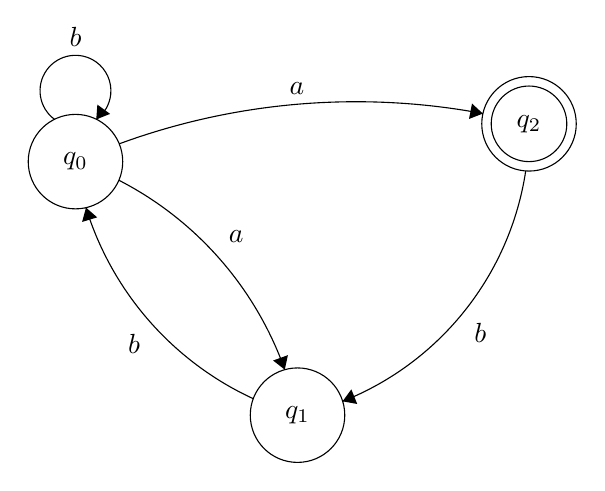
\begin{tikzpicture}[scale=0.2]
            \tikzstyle{every node}+=[inner sep=0pt]
            \draw [black] (10.5,-16.9) circle (3);
            \draw (10.5,-16.9) node {$q_0$};
            \draw [black] (24.6,-33) circle (3);
            \draw (24.6,-33) node {$q_1$};
            \draw [black] (39.3,-14.5) circle (3);
            \draw (39.3,-14.5) node {$q_2$};
            \draw [black] (39.3,-14.5) circle (2.4);
            \draw [black] (13.278,-15.77) arc (110.16418:79.3631:43.633);
            \fill [black] (36.37,-13.85) -- (35.68,-13.21) -- (35.49,-14.19);
            \draw (24.57,-12.68) node [above] {$a$};
            \draw [black] (9.177,-14.22) arc (234:-54:2.25);
            \draw (10.5,-9.65) node [above] {$b$};
            \fill [black] (11.82,-14.22) -- (12.7,-13.87) -- (11.89,-13.28);
            \draw [black] (13.255,-18.082) arc (62.8233:19.59892:21.711);
            \fill [black] (23.79,-30.11) -- (23.99,-29.19) -- (23.05,-29.53);
            \draw (20.21,-21.64) node [right] {$a$};
            \draw [black] (21.791,-31.955) arc (-114.74396:-162.83382:19.791);
            \fill [black] (11.17,-19.82) -- (10.92,-20.73) -- (11.88,-20.44);
            \draw (14.64,-28.47) node [left] {$b$};
            \draw [black] (39.091,-17.489) arc (-8.58948:-68.35145:18.755);
            \fill [black] (27.46,-32.12) -- (28.39,-32.29) -- (28.02,-31.36);
            \draw (35.79,-27.78) node [right] {$b$};
          \end{tikzpicture}
          \end{center}

          Whether this machine will accept $a$ is largely up to how we define acceptance. Generally, NFAs are defined so if there is \emph{any} valid path that leads to a final state, the string will be accepted. So, under that definition, $a$ would be accepted by this NFA.
        \end{ex}

        \subsubsection{Languages Accepted by an NFA}
          Let's define the language $L(N)$ that is accepted by an NFA $N$. Intuitively, we will accept a string $w$ if and only if there is a path from $q_0$ following the letters of $w$ and ending inside $F$.
          \\ \\
          We will extend our formal definition of $\delta$ to $\hat{\delta}: Q \times \Sigma^\star \to \set{ B \subseteq Q }$. $\hat{\delta}(q, w)$ is the set of all states that can be reached from $q$ after reading $w$.
          \\ \\
          For $w = \epsilon$, $\hat{\delta}(q, \epsilon) = \set{q}$. Assume that $\hat{\delta}(q, w)$ is already defined; say $\hat{\delta}(q, w) = \set{q_{i_1}, q_{i_2}, \ldots, q_{i_k}} \subseteq Q$. Now, define $\hat{\delta}(q, wa)$ for any $a \in \Sigma$ as
          $$
            \hat{\delta}(q, wa) = \bigcup_{l = 1}^{k} \delta(q_{i_l}, a)
          $$

          We can then define the language accepted by a particular NFA $N$ as
          $$
            L(N) = \set{ w : \hat{\delta}(q_0, w) \cap F \ne \emptyset }
          $$

          Phrased another way, this set contains all words $w$ which, after reading all characters in $w$, ended up in \emph{at least} one accepting state.

        \subsubsection{Uses of NFAs}
          NFAs sometimes give us a very compact representation of a language that would otherwise be complicated to describe as a DFA.

          \begin{ex}
            NFAs could be used for keyword searches. For example, suppose we want to create an NFA that matches the keywords ``miley'' and ``britney'', and nothing else. We can form this NFA with the alphabet $\Sigma = {a, b, \ldots, z}$:
            \begin{center}
              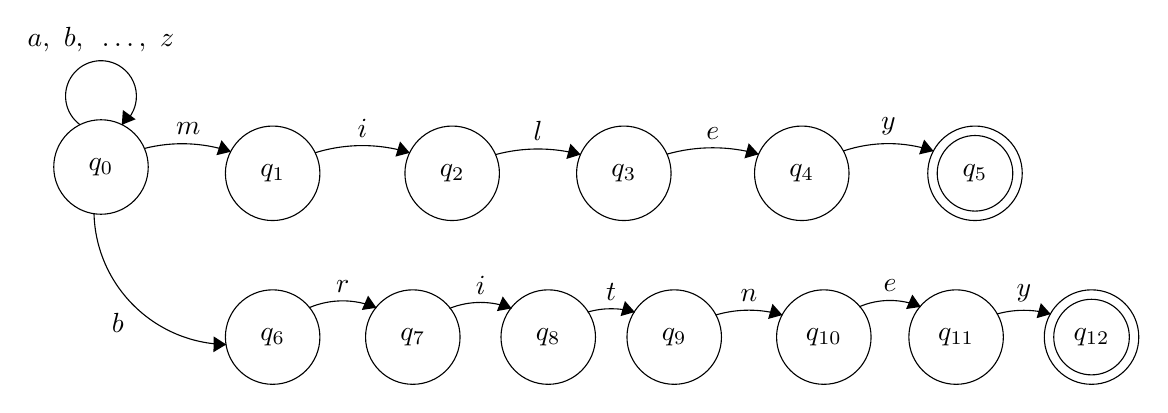
\begin{tikzpicture}[scale=0.2]
                \tikzstyle{every node}+=[inner sep=0pt]
                \draw [black] (10.5,-16.9) circle (3);
                \draw (10.5,-16.9) node {$q_0$};
                \draw [black] (21.4,-17.3) circle (3);
                \draw (21.4,-17.3) node {$q_1$};
                \draw [black] (32.8,-17.3) circle (3);
                \draw (32.8,-17.3) node {$q_2$};
                \draw [black] (43.7,-17.3) circle (3);
                \draw (43.7,-17.3) node {$q_3$};
                \draw [black] (55,-17.3) circle (3);
                \draw (55,-17.3) node {$q_4$};
                \draw [black] (66,-17.3) circle (3);
                \draw (66,-17.3) node {$q_5$};
                \draw [black] (66,-17.3) circle (2.4);
                \draw [black] (21.4,-27.7) circle (3);
                \draw (21.4,-27.7) node {$q_6$};
                \draw [black] (30.3,-27.7) circle (3);
                \draw (30.3,-27.7) node {$q_7$};
                \draw [black] (38.9,-27.7) circle (3);
                \draw (38.9,-27.7) node {$q_8$};
                \draw [black] (46.9,-27.7) circle (3);
                \draw (46.9,-27.7) node {$q_9$};
                \draw [black] (56.4,-27.7) circle (3);
                \draw (56.4,-27.7) node {$q_{10}$};
                \draw [black] (64.8,-27.7) circle (3);
                \draw (64.8,-27.7) node {$q_{11}$};
                \draw [black] (73.4,-27.7) circle (3);
                \draw (73.4,-27.7) node {$q_{12}$};
                \draw [black] (73.4,-27.7) circle (2.4);
                \draw [black] (9.177,-14.22) arc (234:-54:2.25);
                \draw (10.5,-9.65) node [above] {$a,\mbox{ }b,\mbox{ }\ldots,\mbox{ }z$};
                \fill [black] (11.82,-14.22) -- (12.7,-13.87) -- (11.89,-13.28);
                \draw [black] (13.247,-15.724) arc (104.33527:71.46142:9.724);
                \fill [black] (18.75,-15.93) -- (18.15,-15.2) -- (17.83,-16.15);
                \draw (16.05,-14.88) node [above] {$m$};
                \draw [black] (24.091,-15.998) arc (107.31712:72.68288:10.11);
                \fill [black] (30.11,-16) -- (29.49,-15.28) -- (29.2,-16.24);
                \draw (27.1,-15.04) node [above] {$i$};
                \draw [black] (35.544,-16.114) arc (105.09913:74.90087:10.387);
                \fill [black] (40.96,-16.11) -- (40.31,-15.42) -- (40.05,-16.39);
                \draw (38.25,-15.26) node [above] {$l$};
                \draw [black] (46.433,-16.086) arc (105.88913:74.11087:10.656);
                \fill [black] (52.27,-16.09) -- (51.63,-15.39) -- (51.36,-16.35);
                \draw (49.35,-15.18) node [above] {$e$};
                \draw [black] (57.63,-15.886) arc (108.67821:71.32179:8.962);
                \fill [black] (63.37,-15.89) -- (62.77,-15.16) -- (62.45,-16.1);
                \draw (60.5,-14.91) node [above] {$y$};
                \draw [black] (18.453,-28.172) arc (-90.95847:-178.51347:8.544);
                \fill [black] (18.45,-28.17) -- (17.66,-27.66) -- (17.64,-28.66);
                \draw (11.56,-26.18) node [below] {$b$};
                \draw [black] (23.705,-25.839) arc (113.15404:66.84596:5.455);
                \fill [black] (27.99,-25.84) -- (27.46,-25.07) -- (27.06,-25.98);
                \draw (25.85,-24.9) node [above] {$r$};
                \draw [black] (32.633,-25.878) arc (111.77675:68.22325:5.302);
                \fill [black] (36.57,-25.88) -- (36.01,-25.12) -- (35.64,-26.05);
                \draw (34.6,-25) node [above] {$i$};
                \draw [black] (41.4,-26.114) arc (106.30483:73.69517:5.343);
                \fill [black] (44.4,-26.11) -- (43.77,-25.41) -- (43.49,-26.37);
                \draw (42.9,-25.4) node [above] {$t$};
                \draw [black] (49.53,-26.299) arc (106.51296:73.48704:7.458);
                \fill [black] (53.77,-26.3) -- (53.14,-25.59) -- (52.86,-26.55);
                \draw (51.65,-25.49) node [above] {$n$};
                \draw [black] (58.643,-25.777) arc (113.25672:66.74328:4.956);
                \fill [black] (62.56,-25.78) -- (62.02,-25) -- (61.62,-25.92);
                \draw (60.6,-24.87) node [above] {$e$};
                \draw [black] (67.387,-26.237) arc (105.81687:74.18313:6.286);
                \fill [black] (70.81,-26.24) -- (70.18,-25.54) -- (69.91,-26.5);
                \draw (69.1,-25.5) node [above] {$y$};
              \end{tikzpicture}
            \end{center}
          \end{ex}

          \begin{ex}
            Suppose we want to define an NFA for the language $L_n$ = \{$w$ : the $n$th-before-last letter in $w$ is 1\} on the alphabet $\Sigma = \set{0, 1}$. We could form the following NFA to represent this:
            \begin{center}
              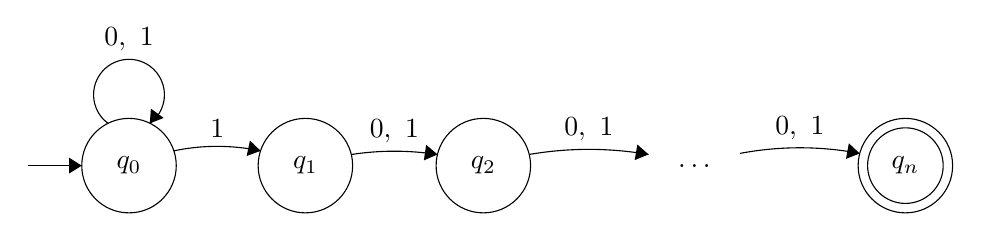
\begin{tikzpicture}[scale=0.2]
                \tikzstyle{every node}+=[inner sep=0pt]
                \draw [black] (12.3,-19.3) circle (3);
                \draw (12.3,-19.3) node {$q_0$};
                \draw [black] (23.5,-19.3) circle (3);
                \draw (23.5,-19.3) node {$q_1$};
                \draw [black] (34.8,-19.3) circle (3);
                \draw (34.8,-19.3) node {$q_2$};
                \draw (48.2,-19.3) node {$\ldots$};
                \draw [black] (61.6,-19.3) circle (3);
                \draw (61.6,-19.3) node {$q_n$};
                \draw [black] (61.6,-19.3) circle (2.4);
                \draw [black] (5.9,-19.3) -- (9.3,-19.3);
                \fill [black] (9.3,-19.3) -- (8.5,-18.8) -- (8.5,-19.8);
                \draw [black] (10.977,-16.62) arc (234:-54:2.25);
                \draw (12.3,-12.05) node [above] {$0,\mbox{ }1$};
                \fill [black] (13.62,-16.62) -- (14.5,-16.27) -- (13.69,-15.68);
                \draw [black] (51.095,-18.525) arc (100.7586:79.2414:20.381);
                \fill [black] (58.7,-18.53) -- (58.01,-17.88) -- (57.83,-18.87);
                \draw (54.9,-17.67) node [above] {$0,\mbox{ }1$};
                \draw [black] (37.713,-18.592) arc (99.80078:80.19922:22.248);
                \fill [black] (45.29,-18.59) -- (44.58,-17.96) -- (44.41,-18.95);
                \draw (41.5,-17.77) node [above] {$0,\mbox{ }1$};
                \draw [black] (26.412,-18.595) arc (98.80333:81.19667:17.888);
                \fill [black] (31.89,-18.59) -- (31.17,-17.98) -- (31.02,-18.97);
                \draw (29.15,-17.88) node [above] {$0,\mbox{ }1$};
                \draw [black] (15.143,-18.362) arc (101.85128:78.14872:13.424);
                \fill [black] (20.66,-18.36) -- (19.98,-17.71) -- (19.77,-18.69);
                \draw (17.9,-17.58) node [above] {$1$};
              \end{tikzpicture}
            \end{center}

            When using an NFA to represent languages like $L_n$, we need just $n + 1$ states.
            \\ \\
            \textbf{Claim}: every DFA that accepts $L_n$ must have at least $2^n$ states. Why? For every word $w$ of length less than $n$, there should be a different state. In other words, if $w_1 \ne w_2$ and $\hat{\delta}(q_0, w_1) = \hat{\delta}(q_0, w_2)$, the DFA is bound to fail. Since $w_1 \ne w_2$, the last ``1'' must be in a different position in $w_1$ and $w_2$, which makes this DFA representation fail.
          \end{ex}

          \textbf{Claim}: a language $L$ has an NFA $N$ such that $L(N) = L$ if and only if there is a DFA $A$ such that $L(A) = A$. In other words, nondeterminism does not increase the power of finite automata.

          \begin{proof}
            First, note that any DFA can also be viewed as an NFA. For every $q \in Q$ and $a \in \Sigma$, if $\delta_N(q, a) = p$, define $\delta_D(q, a) = \set{p}$. In other words, let $\delta_N(q, a) = \set{\delta_D(q, a)}$.
            \\ \\
            For the other direction, if we're given some NFA $N = (\Sigma^N, Q^N, q_0^N, \delta^N, F^N)$, we wish to define a DFA $A = (\Sigma^A, Q^A, q_0^A, \delta^A, F^A)$ such that $L(A) = L(N)$. In particular:
            \begin{itemize}
              \item $\Sigma^A = \Sigma^N$
              \item $Q^A = \set{ B \subseteq Q^N }$
              \item $q_0^A = \set{ q_0^N }$
              \item $\delta^A(q, a) = $ the set of all states that can be reached from $q$ by reading $a$.
              \item $F^A = \set{ B \subseteq Q^N : B \cap F^N \ne \emptyset }$
            \end{itemize}
          \end{proof}

          \begin{ex} \lecture{October 1, 2013}
            Let's look at an example of converting an NFA to an equivalent DFA. Let $N$ be:
            \begin{center}
              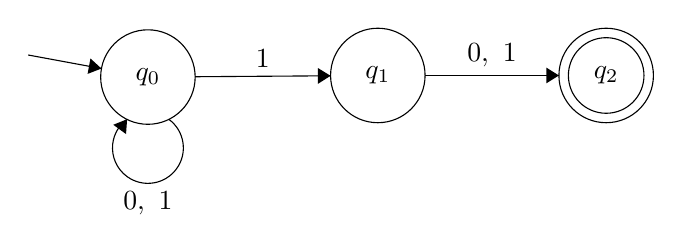
\begin{tikzpicture}[scale=0.2]
                \tikzstyle{every node}+=[inner sep=0pt]
                \draw [black] (11.4,-14.5) circle (3);
                \draw (11.4,-14.5) node {$q_0$};
                \draw [black] (26,-14.4) circle (3);
                \draw (26,-14.4) node {$q_1$};
                \draw [black] (40.5,-14.4) circle (3);
                \draw (40.5,-14.4) node {$q_2$};
                \draw [black] (40.5,-14.4) circle (2.4);
                \draw [black] (3.8,-13.1) -- (8.45,-13.96);
                \fill [black] (8.45,-13.96) -- (7.75,-13.32) -- (7.57,-14.3);
                \draw [black] (12.723,-17.18) arc (54:-234:2.25);
                \draw (11.4,-21.75) node [below] {$0,\mbox{ }1$};
                \fill [black] (10.08,-17.18) -- (9.2,-17.53) -- (10.01,-18.12);
                \draw [black] (14.4,-14.48) -- (23,-14.42);
                \fill [black] (23,-14.42) -- (22.2,-13.93) -- (22.2,-14.93);
                \draw (18.7,-13.94) node [above] {$1$};
                \draw [black] (29,-14.4) -- (37.5,-14.4);
                \fill [black] (37.5,-14.4) -- (36.7,-13.9) -- (36.7,-14.9);
                \draw (33.25,-13.9) node [above] {$0,\mbox{ }1$};
              \end{tikzpicture}
            \end{center}

            $N$ accepts all strings where the second-to-last letter is 1. Note that $N$ is nondeterministic because $q_0$ has two edges for 1, and $q_2$ has no edges. By way of subset construction, we can construct an equivalent DFA:
            \begin{center}
              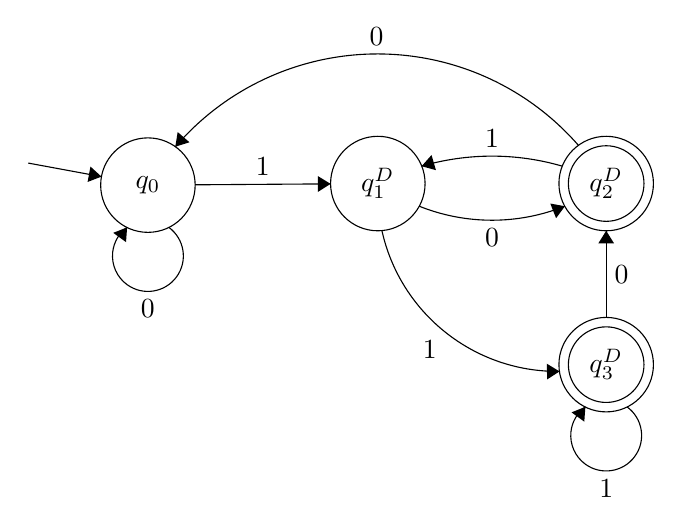
\begin{tikzpicture}[scale=0.2]
                \tikzstyle{every node}+=[inner sep=0pt]
                \draw [black] (11.4,-14.5) circle (3);
                \draw (11.4,-14.5) node {$q_0$};
                \draw [black] (26,-14.4) circle (3);
                \draw (26,-14.4) node {$q_1^D$};
                \draw [black] (40.5,-14.4) circle (3);
                \draw (40.5,-14.4) node {$q_2^D$};
                \draw [black] (40.5,-14.4) circle (2.4);
                \draw [black] (40.5,-25.9) circle (3);
                \draw (40.5,-25.9) node {$q_3^D$};
                \draw [black] (40.5,-25.9) circle (2.4);
                \draw [black] (3.8,-13.1) -- (8.45,-13.96);
                \fill [black] (8.45,-13.96) -- (7.75,-13.32) -- (7.57,-14.3);
                \draw [black] (12.723,-17.18) arc (54:-234:2.25);
                \draw (11.4,-21.75) node [below] {$0$};
                \fill [black] (10.08,-17.18) -- (9.2,-17.53) -- (10.01,-18.12);
                \draw [black] (14.4,-14.48) -- (23,-14.42);
                \fill [black] (23,-14.42) -- (22.2,-13.93) -- (22.2,-14.93);
                \draw (18.7,-13.94) node [above] {$1$};
                \draw [black] (37.875,-15.838) arc (-68.18865:-111.81135:12.449);
                \fill [black] (37.88,-15.84) -- (36.95,-15.67) -- (37.32,-16.6);
                \draw (33.25,-17.23) node [below] {$0$};
                \draw [black] (28.785,-13.296) arc (106.2451:73.7549:15.962);
                \fill [black] (28.78,-13.3) -- (29.69,-13.55) -- (29.41,-12.59);
                \draw (33.25,-12.16) node [above] {$1$};
                \draw [black] (13.144,-12.064) arc (139.32878:41.06501:16.924);
                \fill [black] (13.14,-12.06) -- (14.04,-11.78) -- (13.29,-11.13);
                \draw (25.92,-5.67) node [above] {$0$};
                \draw [black] (41.823,-28.58) arc (54:-234:2.25);
                \draw (40.5,-33.15) node [below] {$1$};
                \fill [black] (39.18,-28.58) -- (38.3,-28.93) -- (39.11,-29.52);
                \draw [black] (37.539,-26.328) arc (-89.29985:-167.53627:11.412);
                \fill [black] (37.54,-26.33) -- (36.73,-25.84) -- (36.75,-26.84);
                \draw (29.3,-24.35) node [below] {$1$};
                \draw [black] (40.5,-22.9) -- (40.5,-17.4);
                \fill [black] (40.5,-17.4) -- (40,-18.2) -- (41,-18.2);
                \draw (41,-20.15) node [right] {$0$};
              \end{tikzpicture}
            \end{center}

            where $q_0^D = \set{q_0}, q_1^D = \set{q_0, q_1}, q_2^D = \set{q_0, q_2}, q_3^D = \set{q_0, q_1, q_2}$.
            \\ \\
            The accepting states of this DFA are all states which contain at least one accepting state from the NFA.
          \end{ex}

          Note that in the worst case, an NFA with $n$ states could be equivalent to a DFA with $2^n$ states. This intuitively follows from the way we construct NFAs -- there are $2^n$ subsets of $n$ items.

      \subsection{Nondeterministic Finite Automata with Epsilon Transitions}
        We will now introduce a third type of machine, \textbf{the $\boldsymbol{\epsilon}$-NFA}. An $\epsilon$-transition is essentially a transition that can occur spontaneously. That is, an $\epsilon$-transition is a transition that can be followed without reading any characters.

        \begin{ex}
          This is what an $\epsilon$-NFA could look like:
          \begin{center}
            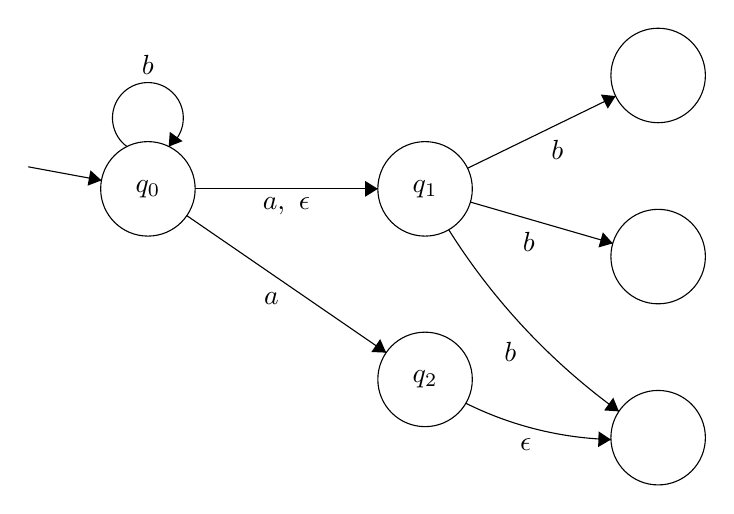
\begin{tikzpicture}[scale=0.2]
              \tikzstyle{every node}+=[inner sep=0pt]
              \draw [black] (11.4,-14.5) circle (3);
              \draw (11.4,-14.5) node {$q_0$};
              \draw [black] (29,-14.5) circle (3);
              \draw (29,-14.5) node {$q_1$};
              \draw [black] (43.8,-7.3) circle (3);
              \draw [black] (43.8,-18.8) circle (3);
              \draw [black] (43.8,-30.3) circle (3);
              \draw [black] (29,-26.6) circle (3);
              \draw (29,-26.6) node {$q_2$};
              \draw [black] (3.8,-13.1) -- (8.45,-13.96);
              \fill [black] (8.45,-13.96) -- (7.75,-13.32) -- (7.57,-14.3);
              \draw [black] (10.077,-11.82) arc (234:-54:2.25);
              \draw (11.4,-7.25) node [above] {$b$};
              \fill [black] (12.72,-11.82) -- (13.6,-11.47) -- (12.79,-10.88);
              \draw [black] (14.4,-14.5) -- (26,-14.5);
              \fill [black] (26,-14.5) -- (25.2,-14) -- (25.2,-15);
              \draw (20.2,-15) node [below] {$a,\mbox{ }\epsilon$};
              \draw [black] (31.7,-13.19) -- (41.1,-8.61);
              \fill [black] (41.1,-8.61) -- (40.16,-8.51) -- (40.6,-9.41);
              \draw (37.39,-11.41) node [below] {$b$};
              \draw [black] (31.88,-15.34) -- (40.92,-17.96);
              \fill [black] (40.92,-17.96) -- (40.29,-17.26) -- (40.01,-18.22);
              \draw (35.58,-17.2) node [below] {$b$};
              \draw [black] (41.308,-28.631) arc (-125.87866:-147.86483:41.443);
              \fill [black] (41.31,-28.63) -- (40.95,-27.76) -- (40.37,-28.57);
              \draw (34.82,-24.85) node [left] {$b$};
              \draw [black] (13.87,-16.2) -- (26.53,-24.9);
              \fill [black] (26.53,-24.9) -- (26.15,-24.04) -- (25.59,-24.86);
              \draw (19.25,-21.05) node [below] {$a$};
              \draw [black] (40.805,-30.418) arc (-91.63068:-116.44181:22.112);
              \fill [black] (40.8,-30.42) -- (40.02,-29.9) -- (39.99,-30.9);
              \draw (35.39,-30.33) node [below] {$\epsilon$};
            \end{tikzpicture}
          \end{center}
        \end{ex}

        Let's consider a more simplistic example to understand $\epsilon$-NFAs better.
        \begin{ex}
          Consider $N_1$:
          \begin{center}
            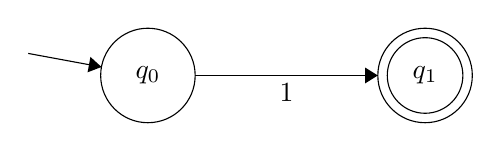
\begin{tikzpicture}[scale=0.2]
              \tikzstyle{every node}+=[inner sep=0pt]
              \draw [black] (11.4,-14.5) circle (3);
              \draw (11.4,-14.5) node {$q_0$};
              \draw [black] (29,-14.5) circle (3);
              \draw (29,-14.5) node {$q_1$};
              \draw [black] (29,-14.5) circle (2.4);
              \draw [black] (3.8,-13.1) -- (8.45,-13.96);
              \fill [black] (8.45,-13.96) -- (7.75,-13.32) -- (7.57,-14.3);
              \draw [black] (14.4,-14.5) -- (26,-14.5);
              \fill [black] (26,-14.5) -- (25.2,-14) -- (25.2,-15);
              \draw (20.2,-15) node [below] {$1$};
            \end{tikzpicture}
          \end{center}

          It's trivial to see that $L(N_1) = \set{1}$. Now, consider $N_2$, the same NFA but adding an $\epsilon$-transition:
          \begin{center}
            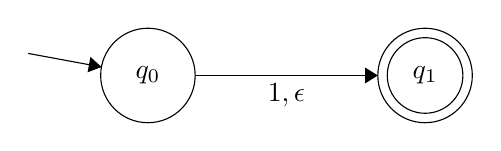
\begin{tikzpicture}[scale=0.2]
              \tikzstyle{every node}+=[inner sep=0pt]
              \draw [black] (11.4,-14.5) circle (3);
              \draw (11.4,-14.5) node {$q_0$};
              \draw [black] (29,-14.5) circle (3);
              \draw (29,-14.5) node {$q_1$};
              \draw [black] (29,-14.5) circle (2.4);
              \draw [black] (3.8,-13.1) -- (8.45,-13.96);
              \fill [black] (8.45,-13.96) -- (7.75,-13.32) -- (7.57,-14.3);
              \draw [black] (14.4,-14.5) -- (26,-14.5);
              \fill [black] (26,-14.5) -- (25.2,-14) -- (25.2,-15);
              \draw (20.2,-15) node [below] {$1, \epsilon$};
            \end{tikzpicture}
          \end{center}

          Note that now, $L(N_2) = \set{\epsilon, 1}$. That is, $L(N_2)$ contains the empty string, and the string that is just a single 1.
          \\ \\
          Let's now consider a different NFA, $N_3$:
          \begin{center}
            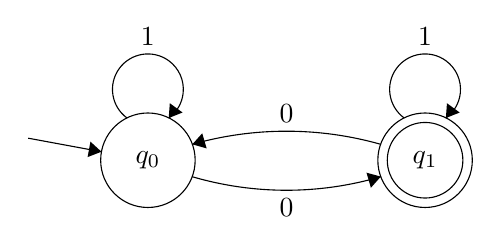
\begin{tikzpicture}[scale=0.2]
              \tikzstyle{every node}+=[inner sep=0pt]
              \draw [black] (11.4,-14.5) circle (3);
              \draw (11.4,-14.5) node {$q_0$};
              \draw [black] (29,-14.5) circle (3);
              \draw (29,-14.5) node {$q_1$};
              \draw [black] (29,-14.5) circle (2.4);
              \draw [black] (3.8,-13.1) -- (8.45,-13.96);
              \fill [black] (8.45,-13.96) -- (7.75,-13.32) -- (7.57,-14.3);
              \draw [black] (26.19,-15.545) arc (-73.64114:-106.35886:21.269);
              \fill [black] (26.19,-15.54) -- (25.28,-15.29) -- (25.56,-16.25);
              \draw (20.2,-16.91) node [below] {$0$};
              \draw [black] (14.221,-13.487) arc (105.83465:74.16535:21.911);
              \fill [black] (14.22,-13.49) -- (15.13,-13.75) -- (14.85,-12.79);
              \draw (20.2,-12.16) node [above] {$0$};
              \draw [black] (10.077,-11.82) arc (234:-54:2.25);
              \draw (11.4,-7.25) node [above] {$1$};
              \fill [black] (12.72,-11.82) -- (13.6,-11.47) -- (12.79,-10.88);
              \draw [black] (27.677,-11.82) arc (234:-54:2.25);
              \draw (29,-7.25) node [above] {$1$};
              \fill [black] (30.32,-11.82) -- (31.2,-11.47) -- (30.39,-10.88);
            \end{tikzpicture}
          \end{center}

          $L(N_3) = \set{ w : \#_0(w) \text{ is odd}}$. Finally, let's consider $N_4$, the same NFA but with an $\epsilon$-transition added:
          \begin{center}
            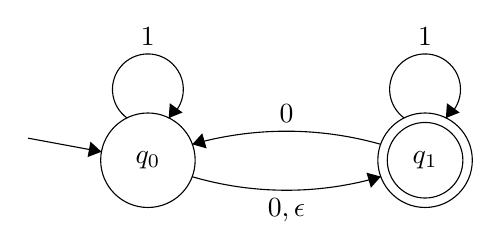
\begin{tikzpicture}[scale=0.2]
              \tikzstyle{every node}+=[inner sep=0pt]
              \draw [black] (11.4,-14.5) circle (3);
              \draw (11.4,-14.5) node {$q_0$};
              \draw [black] (29,-14.5) circle (3);
              \draw (29,-14.5) node {$q_1$};
              \draw [black] (29,-14.5) circle (2.4);
              \draw [black] (3.8,-13.1) -- (8.45,-13.96);
              \fill [black] (8.45,-13.96) -- (7.75,-13.32) -- (7.57,-14.3);
              \draw [black] (26.19,-15.545) arc (-73.64114:-106.35886:21.269);
              \fill [black] (26.19,-15.54) -- (25.28,-15.29) -- (25.56,-16.25);
              \draw (20.2,-16.91) node [below] {$0,\epsilon$};
              \draw [black] (14.221,-13.487) arc (105.83465:74.16535:21.911);
              \fill [black] (14.22,-13.49) -- (15.13,-13.75) -- (14.85,-12.79);
              \draw (20.2,-12.16) node [above] {$0$};
              \draw [black] (10.077,-11.82) arc (234:-54:2.25);
              \draw (11.4,-7.25) node [above] {$1$};
              \fill [black] (12.72,-11.82) -- (13.6,-11.47) -- (12.79,-10.88);
              \draw [black] (27.677,-11.82) arc (234:-54:2.25);
              \draw (29,-7.25) node [above] {$1$};
              \fill [black] (30.32,-11.82) -- (31.2,-11.47) -- (30.39,-10.88);
            \end{tikzpicture}
          \end{center}

          $N_4$ accepts everything. That is, $L(N_4) = \set{0, 1}^\star$. In $N_4$, we can spontaneously move to $q_1$ initially. Then, either $1$ loops in $q_1$ or you follow $0$ to $q_0$, but in that case you can spontaneously move back to $q_1$ again.
        \end{ex}

        We can define an $\epsilon$-NFA as follows. For such a machine $N$, $L(N)$ = \{$w$ : there is a way that upon reading $w$ and using $\epsilon$-transitions, $q_0$ leads to some accepting state\}.
        \\ \\
        \textbf{Claim}: a language is accepted by an $\epsilon$-NFA if and only if it is accepted by some DFA.
        \\ \\
        The proof of this claim is the same as before, except additionally taking the $\epsilon$-transitions into account when performing the subset construction of the DFA.
        \\ \\
        Recall the theorem we discussed a few weeks ago:
        \begin{theorem}
          For every regular expression $r$, there exists a DFA $A$ such that $L(r) = L(A)$.
        \end{theorem}

        \begin{proof}
          We will prove this theorem by structural induction on the set of regular expressions.
          \\ \\
          Let's prove an equivalent claim:
          \\ \\
          \textbf{Claim}: for every $r$, there is a DFA $A$ such that $A$ has only a single accepting state, no edges leading out of the accepting state, but $A$ may have $\epsilon$-transitions, and $L(r) = L(A)$. (Note that this isn't formally a DFA, since we allow $\epsilon$-transitions and missing edges, but since every $\epsilon$-NFA is equivalent to a DFA, we know that a corresponding \emph{proper} DFA exists.)
          \\ \\
          \textbf{Induction basis}: $\emptyset, \epsilon$, and $a$ for $a \in \Sigma$.
          \\ \\
          An $\epsilon$-DFA for $L(\emptyset) = \emptyset$ is:
          \begin{center}
            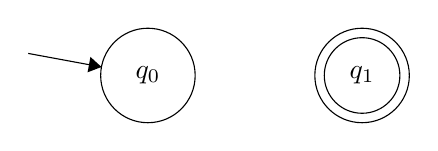
\begin{tikzpicture}[scale=0.2]
              \tikzstyle{every node}+=[inner sep=0pt]
              \draw [black] (11.4,-14.5) circle (3);
              \draw (11.4,-14.5) node {$q_0$};
              \draw [black] (25,-14.5) circle (3);
              \draw (25,-14.5) node {$q_1$};
              \draw [black] (25,-14.5) circle (2.4);
              \draw [black] (3.8,-13.1) -- (8.45,-13.96);
              \fill [black] (8.45,-13.96) -- (7.75,-13.32) -- (7.57,-14.3);
            \end{tikzpicture}
          \end{center}

          An $\epsilon$-DFA for $L(\epsilon) = \set{\epsilon}$ is:
          \begin{center}
            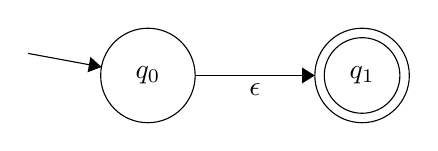
\begin{tikzpicture}[scale=0.2]
              \tikzstyle{every node}+=[inner sep=0pt]
              \draw [black] (11.4,-14.5) circle (3);
              \draw (11.4,-14.5) node {$q_0$};
              \draw [black] (25,-14.5) circle (3);
              \draw (25,-14.5) node {$q_1$};
              \draw [black] (25,-14.5) circle (2.4);
              \draw [black] (3.8,-13.1) -- (8.45,-13.96);
              \fill [black] (8.45,-13.96) -- (7.75,-13.32) -- (7.57,-14.3);
              \draw [black] (14.4,-14.5) -- (22,-14.5);
              \fill [black] (22,-14.5) -- (21.2,-14) -- (21.2,-15);
              \draw (18.2,-15) node [below] {$\epsilon$};
            \end{tikzpicture}
          \end{center}

          An $\epsilon$-DFA for $L(a) = \set{a}$ is:
          \begin{center}
            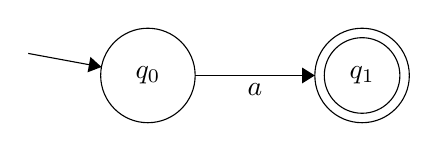
\begin{tikzpicture}[scale=0.2]
              \tikzstyle{every node}+=[inner sep=0pt]
              \draw [black] (11.4,-14.5) circle (3);
              \draw (11.4,-14.5) node {$q_0$};
              \draw [black] (25,-14.5) circle (3);
              \draw (25,-14.5) node {$q_1$};
              \draw [black] (25,-14.5) circle (2.4);
              \draw [black] (3.8,-13.1) -- (8.45,-13.96);
              \fill [black] (8.45,-13.96) -- (7.75,-13.32) -- (7.57,-14.3);
              \draw [black] (14.4,-14.5) -- (22,-14.5);
              \fill [black] (22,-14.5) -- (21.2,-14) -- (21.2,-15);
              \draw (18.2,-15) node [below] {$a$};
            \end{tikzpicture}
          \end{center}

          \textbf{Induction step}: assume $r_1, r_2$ are regular expressions such that there are $A_1, A_2$ for which $L(r_1) = L(A_1)$ and $L(r_2) = L(A_2)$. Recall the operations that we defined on regular expressions:

          \begin{center}
            $P = $ \bigg\{ \AxiomC{$r_1$} \AxiomC{$r_2$} \BinaryInfC{$r_1 + r_2$} \DisplayProof, \AxiomC{$r_1$} \AxiomC{$r_2$} \BinaryInfC{$r_1 r_2$} \DisplayProof, \AxiomC{$r_1$} \UnaryInfC{$(r_1)$} \DisplayProof, \AxiomC{$r_1$} \UnaryInfC{$r_1^\star$} \DisplayProof \bigg\}
          \end{center}

          We must show that our claim holds for each of these operations.
          \\ \\
          Let's consider the first operation, \AxiomC{$r_1$} \AxiomC{$r_2$} \BinaryInfC{$r_1 + r_2$} \DisplayProof. We need to construct an automaton $A_3$ such that $L(A_3) = L(A_1) \cup L(A_2)$. Essentially, we want to introduce a new $q_0$ that is connected via $\epsilon$-transitions to the $q_0$ states of $A_1$ and $A_2$. Then, convert the single final state of each of $A_1$ and $A_2$ into a non-final state, but connect that state via an $\epsilon$-transition to a new accepting state. Here's a visualization of this construction:
          \begin{center}
            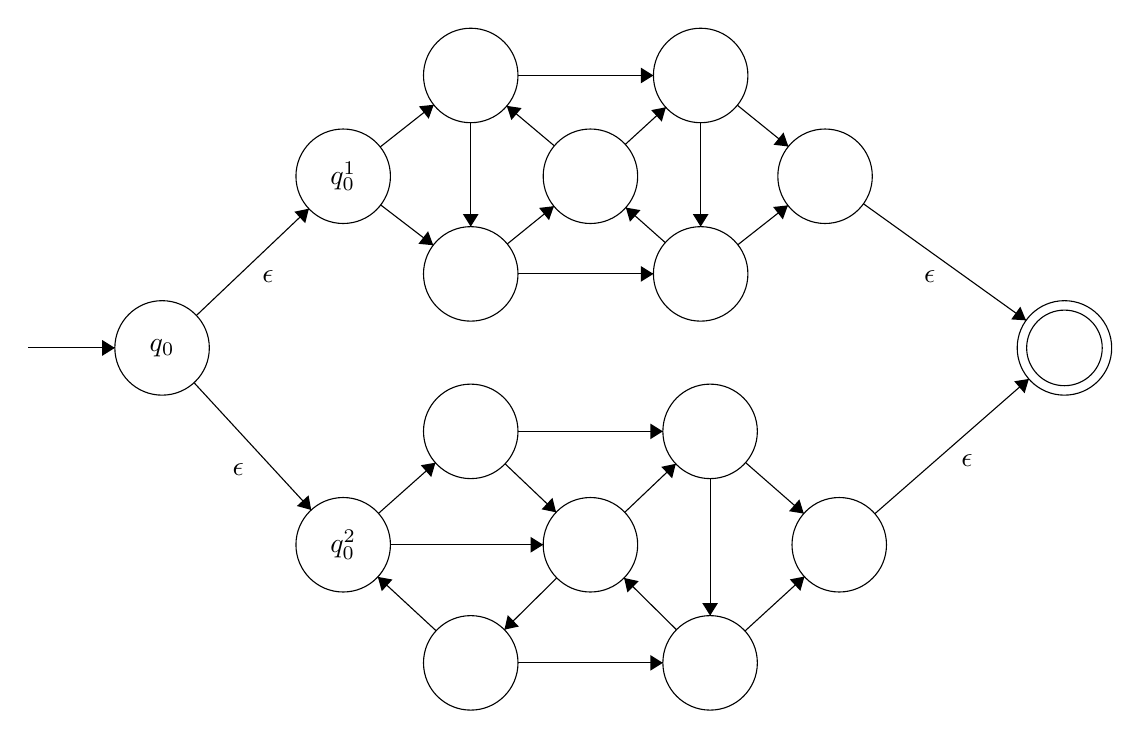
\begin{tikzpicture}[scale=0.2]
              \tikzstyle{every node}+=[inner sep=0pt]
              \draw [black] (13.5,-28.5) circle (3);
              \draw (13.5,-28.5) node {$q_0$};
              \draw [black] (25,-17.6) circle (3);
              \draw (25,-17.6) node {$q_0^1$};
              \draw [black] (40.7,-17.6) circle (3);
              \draw [black] (55.6,-17.6) circle (3);
              \draw [black] (47.7,-23.8) circle (3);
              \draw [black] (33.1,-23.8) circle (3);
              \draw [black] (47.7,-11.2) circle (3);
              \draw [black] (33.1,-11.2) circle (3);
              \draw [black] (25,-41) circle (3);
              \draw (25,-41) node {$q_0^2$};
              \draw [black] (33.1,-33.8) circle (3);
              \draw [black] (33.1,-48.5) circle (3);
              \draw [black] (40.7,-41) circle (3);
              \draw [black] (48.3,-33.8) circle (3);
              \draw [black] (48.3,-48.5) circle (3);
              \draw [black] (56.5,-41) circle (3);
              \draw [black] (70.8,-28.5) circle (3);
              \draw [black] (70.8,-28.5) circle (2.4);
              \draw [black] (5,-28.5) -- (10.5,-28.5);
              \fill [black] (10.5,-28.5) -- (9.7,-28) -- (9.7,-29);
              \draw [black] (15.68,-26.44) -- (22.82,-19.66);
              \fill [black] (22.82,-19.66) -- (21.9,-19.85) -- (22.59,-20.58);
              \draw (20.22,-23.53) node [below] {$\epsilon$};
              \draw [black] (15.53,-30.71) -- (22.97,-38.79);
              \fill [black] (22.97,-38.79) -- (22.8,-37.86) -- (22.06,-38.54);
              \draw (18.72,-36.21) node [left] {$\epsilon$};
              \draw [black] (27.35,-15.74) -- (30.75,-13.06);
              \fill [black] (30.75,-13.06) -- (29.81,-13.16) -- (30.43,-13.95);
              \draw [black] (27.38,-19.42) -- (30.72,-21.98);
              \fill [black] (30.72,-21.98) -- (30.39,-21.09) -- (29.78,-21.89);
              \draw [black] (35.42,-21.9) -- (38.38,-19.5);
              \fill [black] (38.38,-19.5) -- (37.44,-19.61) -- (38.07,-20.39);
              \draw [black] (36.1,-23.8) -- (44.7,-23.8);
              \fill [black] (44.7,-23.8) -- (43.9,-23.3) -- (43.9,-24.3);
              \draw [black] (36.1,-11.2) -- (44.7,-11.2);
              \fill [black] (44.7,-11.2) -- (43.9,-10.7) -- (43.9,-11.7);
              \draw [black] (42.91,-15.58) -- (45.49,-13.22);
              \fill [black] (45.49,-13.22) -- (44.56,-13.4) -- (45.23,-14.13);
              \draw [black] (50.03,-13.09) -- (53.27,-15.71);
              \fill [black] (53.27,-15.71) -- (52.96,-14.82) -- (52.33,-15.6);
              \draw [black] (50.06,-21.95) -- (53.24,-19.45);
              \fill [black] (53.24,-19.45) -- (52.3,-19.55) -- (52.92,-20.34);
              \draw [black] (27.24,-39.01) -- (30.86,-35.79);
              \fill [black] (30.86,-35.79) -- (29.93,-35.95) -- (30.59,-36.7);
              \draw [black] (28,-41) -- (37.7,-41);
              \fill [black] (37.7,-41) -- (36.9,-40.5) -- (36.9,-41.5);
              \draw [black] (38.56,-43.11) -- (35.24,-46.39);
              \fill [black] (35.24,-46.39) -- (36.16,-46.19) -- (35.45,-45.47);
              \draw [black] (36.1,-48.5) -- (45.3,-48.5);
              \fill [black] (45.3,-48.5) -- (44.5,-48) -- (44.5,-49);
              \draw [black] (36.1,-33.8) -- (45.3,-33.8);
              \fill [black] (45.3,-33.8) -- (44.5,-33.3) -- (44.5,-34.3);
              \draw [black] (42.88,-38.94) -- (46.12,-35.86);
              \fill [black] (46.12,-35.86) -- (45.2,-36.05) -- (45.89,-36.78);
              \draw [black] (50.55,-35.78) -- (54.25,-39.02);
              \fill [black] (54.25,-39.02) -- (53.97,-38.12) -- (53.31,-38.87);
              \draw [black] (50.51,-46.48) -- (54.29,-43.02);
              \fill [black] (54.29,-43.02) -- (53.36,-43.2) -- (54.03,-43.93);
              \draw [black] (46.16,-46.39) -- (42.84,-43.11);
              \fill [black] (42.84,-43.11) -- (43.05,-44.03) -- (43.76,-43.31);
              \draw [black] (58.76,-39.03) -- (68.54,-30.47);
              \fill [black] (68.54,-30.47) -- (67.61,-30.62) -- (68.27,-31.38);
              \draw (64.61,-35.24) node [below] {$\epsilon$};
              \draw [black] (58.04,-19.35) -- (68.36,-26.75);
              \fill [black] (68.36,-26.75) -- (68,-25.88) -- (67.42,-26.69);
              \draw (62.25,-23.55) node [below] {$\epsilon$};
              \draw [black] (30.9,-46.46) -- (27.2,-43.04);
              \fill [black] (27.2,-43.04) -- (27.45,-43.95) -- (28.13,-43.21);
              \draw [black] (48.3,-36.8) -- (48.3,-45.5);
              \fill [black] (48.3,-45.5) -- (48.8,-44.7) -- (47.8,-44.7);
              \draw [black] (45.45,-21.81) -- (42.95,-19.59);
              \fill [black] (42.95,-19.59) -- (43.21,-20.49) -- (43.88,-19.75);
              \draw [black] (47.7,-14.2) -- (47.7,-20.8);
              \fill [black] (47.7,-20.8) -- (48.2,-20) -- (47.2,-20);
              \draw [black] (35.28,-35.86) -- (38.52,-38.94);
              \fill [black] (38.52,-38.94) -- (38.29,-38.02) -- (37.6,-38.75);
              \draw [black] (38.41,-15.67) -- (35.39,-13.13);
              \fill [black] (35.39,-13.13) -- (35.68,-14.03) -- (36.33,-13.27);
              \draw [black] (33.1,-14.2) -- (33.1,-20.8);
              \fill [black] (33.1,-20.8) -- (33.6,-20) -- (32.6,-20);
            \end{tikzpicture}
          \end{center}

          Next, let's look at the operation \AxiomC{$r_1$} \AxiomC{$r_2$} \BinaryInfC{$r_1 r_2$} \DisplayProof. We need to construct an automaton $A_4$ such that $L(A_4) = L(A_1) L(A_2)$. Essentially, we want to make the final states of $A_1$ and $A_2$ non-final, then connect the final state of $A_1$ to the $q_0$ of $A_2$, through an $\epsilon$-transition. Then, the previously-final state of $A_2$ should connect to a new final state through an $\epsilon$-transition. Here's a visualization of this construction:
          \begin{center}
            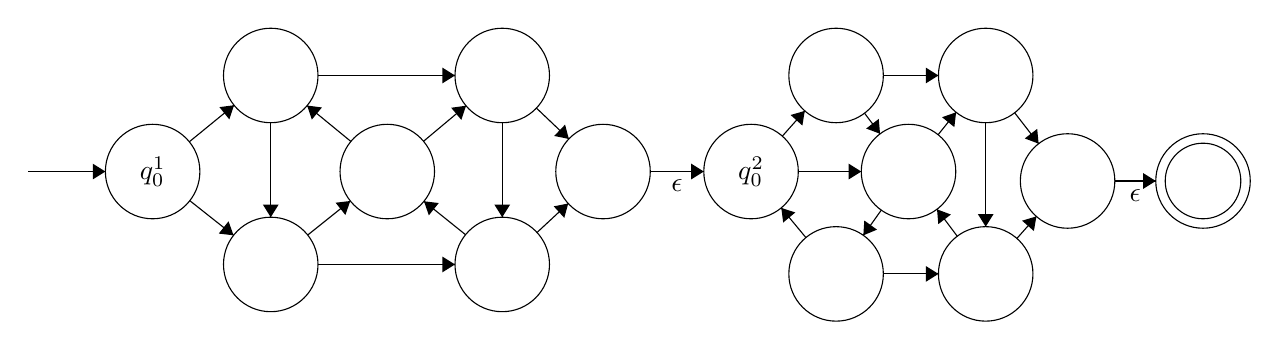
\begin{tikzpicture}[scale=0.2]
              \tikzstyle{every node}+=[inner sep=0pt]
              \draw [black] (9.9,-27.9) circle (3);
              \draw (9.9,-27.9) node {$q_0^1$};
              \draw [black] (24.8,-27.9) circle (3);
              \draw [black] (38.5,-27.9) circle (3);
              \draw [black] (32.1,-33.8) circle (3);
              \draw [black] (17.4,-33.8) circle (3);
              \draw [black] (32.1,-21.8) circle (3);
              \draw [black] (17.4,-21.8) circle (3);
              \draw [black] (47.9,-27.9) circle (3);
              \draw (47.9,-27.9) node {$q_0^2$};
              \draw [black] (53.3,-21.8) circle (3);
              \draw [black] (53.3,-34.4) circle (3);
              \draw [black] (57.9,-27.9) circle (3);
              \draw [black] (62.8,-21.8) circle (3);
              \draw [black] (62.8,-34.4) circle (3);
              \draw [black] (68,-28.5) circle (3);
              \draw [black] (76.6,-28.5) circle (3);
              \draw [black] (76.6,-28.5) circle (2.4);
              \draw [black] (12.23,-26.01) -- (15.07,-23.69);
              \fill [black] (15.07,-23.69) -- (14.14,-23.81) -- (14.77,-24.59);
              \draw [black] (12.26,-29.75) -- (15.04,-31.95);
              \fill [black] (15.04,-31.95) -- (14.72,-31.06) -- (14.1,-31.84);
              \draw [black] (19.75,-31.93) -- (22.45,-29.77);
              \fill [black] (22.45,-29.77) -- (21.52,-29.88) -- (22.14,-30.66);
              \draw [black] (20.4,-33.8) -- (29.1,-33.8);
              \fill [black] (29.1,-33.8) -- (28.3,-33.3) -- (28.3,-34.3);
              \draw [black] (20.4,-21.8) -- (29.1,-21.8);
              \fill [black] (29.1,-21.8) -- (28.3,-21.3) -- (28.3,-22.3);
              \draw [black] (27.1,-25.98) -- (29.8,-23.72);
              \fill [black] (29.8,-23.72) -- (28.86,-23.85) -- (29.5,-24.62);
              \draw [black] (34.27,-23.87) -- (36.33,-25.83);
              \fill [black] (36.33,-25.83) -- (36.09,-24.92) -- (35.4,-25.64);
              \draw [black] (34.31,-31.77) -- (36.29,-29.93);
              \fill [black] (36.29,-29.93) -- (35.37,-30.11) -- (36.04,-30.84);
              \draw [black] (49.89,-25.65) -- (51.31,-24.05);
              \fill [black] (51.31,-24.05) -- (50.41,-24.31) -- (51.16,-24.98);
              \draw [black] (50.9,-27.9) -- (54.9,-27.9);
              \fill [black] (54.9,-27.9) -- (54.1,-27.4) -- (54.1,-28.4);
              \draw [black] (56.17,-30.35) -- (55.03,-31.95);
              \fill [black] (55.03,-31.95) -- (55.9,-31.59) -- (55.09,-31.01);
              \draw [black] (56.3,-34.4) -- (59.8,-34.4);
              \fill [black] (59.8,-34.4) -- (59,-33.9) -- (59,-34.9);
              \draw [black] (56.3,-21.8) -- (59.8,-21.8);
              \fill [black] (59.8,-21.8) -- (59,-21.3) -- (59,-22.3);
              \draw [black] (59.78,-25.56) -- (60.92,-24.14);
              \fill [black] (60.92,-24.14) -- (60.03,-24.45) -- (60.81,-25.08);
              \draw [black] (64.64,-24.17) -- (66.16,-26.13);
              \fill [black] (66.16,-26.13) -- (66.07,-25.19) -- (65.28,-25.8);
              \draw [black] (64.78,-32.15) -- (66.02,-30.75);
              \fill [black] (66.02,-30.75) -- (65.11,-31.02) -- (65.86,-31.68);
              \draw [black] (60.99,-32) -- (59.71,-30.3);
              \fill [black] (59.71,-30.3) -- (59.79,-31.24) -- (60.59,-30.63);
              \draw [black] (51.38,-32.09) -- (49.82,-30.21);
              \fill [black] (49.82,-30.21) -- (49.94,-31.14) -- (50.71,-30.5);
              \draw [black] (62.8,-24.8) -- (62.8,-31.4);
              \fill [black] (62.8,-31.4) -- (63.3,-30.6) -- (62.3,-30.6);
              \draw [black] (29.77,-31.91) -- (27.13,-29.79);
              \fill [black] (27.13,-29.79) -- (27.44,-30.68) -- (28.07,-29.9);
              \draw [black] (32.1,-24.8) -- (32.1,-30.8);
              \fill [black] (32.1,-30.8) -- (32.6,-30) -- (31.6,-30);
              \draw [black] (55.11,-24.2) -- (56.09,-25.5);
              \fill [black] (56.09,-25.5) -- (56.01,-24.56) -- (55.21,-25.17);
              \draw [black] (22.49,-25.99) -- (19.71,-23.71);
              \fill [black] (19.71,-23.71) -- (20.01,-24.6) -- (20.65,-23.83);
              \draw [black] (17.4,-24.8) -- (17.4,-30.8);
              \fill [black] (17.4,-30.8) -- (17.9,-30) -- (16.9,-30);
              \draw [black] (71,-28.5) -- (73.6,-28.5);
              \fill [black] (73.6,-28.5) -- (72.8,-28) -- (72.8,-29);
              \draw (72.3,-29) node [below] {$\epsilon$};
              \draw [black] (41.5,-27.9) -- (44.9,-27.9);
              \fill [black] (44.9,-27.9) -- (44.1,-27.4) -- (44.1,-28.4);
              \draw (43.2,-28.4) node [below] {$\epsilon$};
              \draw [black] (2,-27.9) -- (6.9,-27.9);
              \fill [black] (6.9,-27.9) -- (6.1,-27.4) -- (6.1,-28.4);
            \end{tikzpicture}
          \end{center}

          The operation \AxiomC{$r_1$} \UnaryInfC{$(r_1)$} \DisplayProof is trivially true. The DFA for this operation is the same as the DFA for $r_1$.
          \\ \\
          Finally, let's look at our last operation, \AxiomC{$r_1$} \UnaryInfC{$r_1^\star$} \DisplayProof. Assume $L(A) = L(r)$. We will define $A^\star$, an $\epsilon$-DFA such that $L(A^\star) = L(r^\star) = (L(r))^\star$.
          \\ \\
          We will introduce a new initial state, $q_0$, and a new accepting state. We will connect $q_0$ and our new accepting state by an $\epsilon$-transition, since $\epsilon \in L(r^\star)$. We will connect our $q_0$ to the initial state of $A$ by an $\epsilon$-transition. We will make the final state of $A$ non-final, and connect it back to $A$'s previously-initial state ($A$'s $q_0$) by an $\epsilon$-transition, to allow repetition. Finally, we will connect the previously-final state of $A$ to our new accepting state by an $\epsilon$-transition. Here's a visualization of this construction:
          \begin{center}
            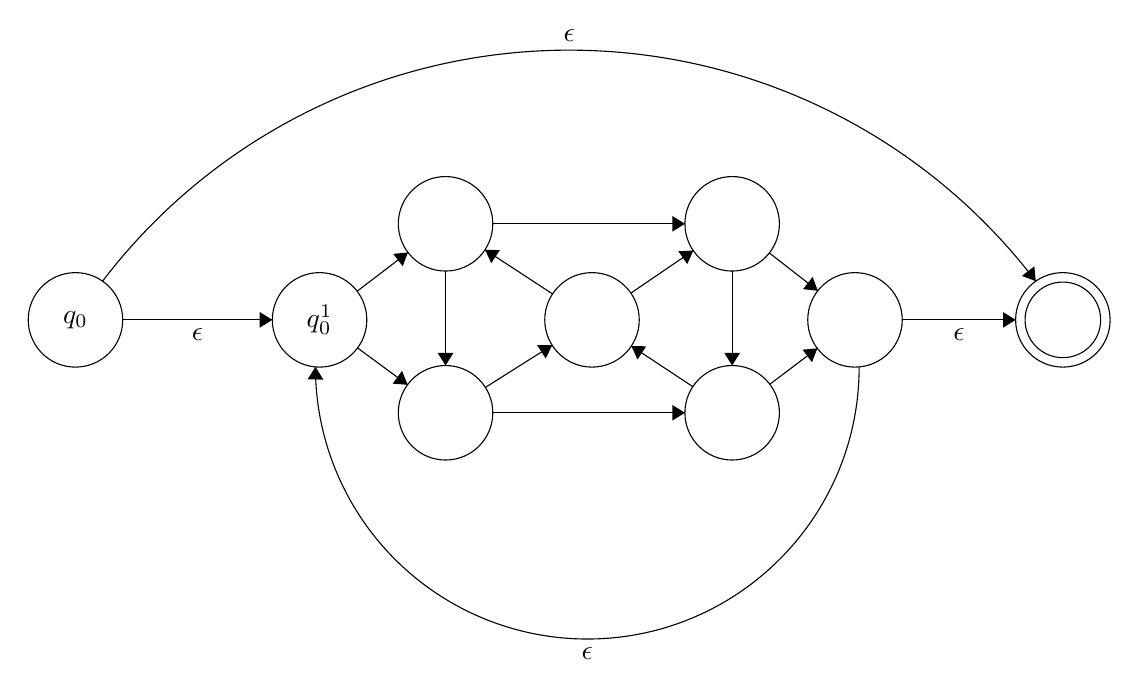
\begin{tikzpicture}[scale=0.2]
              \tikzstyle{every node}+=[inner sep=0pt]
              \draw [black] (27.9,-27.9) circle (3);
              \draw (27.9,-27.9) node {$q_0^1$};
              \draw [black] (45.2,-27.9) circle (3);
              \draw [black] (61.9,-27.9) circle (3);
              \draw [black] (54.1,-33.8) circle (3);
              \draw [black] (35.9,-33.8) circle (3);
              \draw [black] (54.1,-21.8) circle (3);
              \draw [black] (35.9,-21.8) circle (3);
              \draw [black] (75.1,-27.9) circle (3);
              \draw [black] (75.1,-27.9) circle (2.4);
              \draw [black] (12.4,-27.9) circle (3);
              \draw (12.4,-27.9) node {$q_0$};
              \draw [black] (30.29,-26.08) -- (33.51,-23.62);
              \fill [black] (33.51,-23.62) -- (32.58,-23.71) -- (33.18,-24.5);
              \draw [black] (30.31,-29.68) -- (33.49,-32.02);
              \fill [black] (33.49,-32.02) -- (33.14,-31.14) -- (32.54,-31.95);
              \draw [black] (38.43,-32.19) -- (42.67,-29.51);
              \fill [black] (42.67,-29.51) -- (41.72,-29.51) -- (42.26,-30.36);
              \draw [black] (38.9,-33.8) -- (51.1,-33.8);
              \fill [black] (51.1,-33.8) -- (50.3,-33.3) -- (50.3,-34.3);
              \draw [black] (38.9,-21.8) -- (51.1,-21.8);
              \fill [black] (51.1,-21.8) -- (50.3,-21.3) -- (50.3,-22.3);
              \draw [black] (47.67,-26.2) -- (51.63,-23.5);
              \fill [black] (51.63,-23.5) -- (50.68,-23.54) -- (51.25,-24.36);
              \draw [black] (56.46,-23.65) -- (59.54,-26.05);
              \fill [black] (59.54,-26.05) -- (59.21,-25.17) -- (58.6,-25.95);
              \draw [black] (56.49,-31.99) -- (59.51,-29.71);
              \fill [black] (59.51,-29.71) -- (58.57,-29.79) -- (59.17,-30.59);
              \draw [black] (51.6,-32.14) -- (47.7,-29.56);
              \fill [black] (47.7,-29.56) -- (48.09,-30.42) -- (48.64,-29.58);
              \draw [black] (54.1,-24.8) -- (54.1,-30.8);
              \fill [black] (54.1,-30.8) -- (54.6,-30) -- (53.6,-30);
              \draw [black] (42.69,-26.25) -- (38.41,-23.45);
              \fill [black] (38.41,-23.45) -- (38.8,-24.3) -- (39.35,-23.47);
              \draw [black] (35.9,-24.8) -- (35.9,-30.8);
              \fill [black] (35.9,-30.8) -- (36.4,-30) -- (35.4,-30);
              \draw [black] (15.4,-27.9) -- (24.9,-27.9);
              \fill [black] (24.9,-27.9) -- (24.1,-27.4) -- (24.1,-28.4);
              \draw (20.15,-28.4) node [below] {$\epsilon$};
              \draw [black] (62.163,-30.885) arc (0.06123:-180.06123:17.263);
              \fill [black] (27.64,-30.88) -- (27.14,-31.68) -- (28.14,-31.69);
              \draw (44.9,-48.67) node [below] {$\epsilon$};
              \draw [black] (14.121,-25.443) arc (142.68364:37.31636:37.256);
              \fill [black] (73.38,-25.44) -- (73.29,-24.5) -- (72.5,-25.11);
              \draw (43.75,-10.27) node [above] {$\epsilon$};
              \draw [black] (64.9,-27.9) -- (72.1,-27.9);
              \fill [black] (72.1,-27.9) -- (71.3,-27.4) -- (71.3,-28.4);
              \draw (68.5,-28.4) node [below] {$\epsilon$};
            \end{tikzpicture}
          \end{center}
        \end{proof}

        \begin{ex}
          Consider the regular expression $r = (0 + 1)^\star 1(0 + 1)$. This expression matches all strings with their second-to-last character being 1.
          \\ \\
          Let's construct an $\epsilon$-DFA $A$ such that $L(A) = L(r)$, by following the steps of the previous proof.
          \\ \\
          We would typically generate the regular expression $r$ in the following order:
          \begin{align*}
            0 \\
            1 \\
            (0 + 1) \\
            (0 + 1)^\star \\
            (0 + 1)^\star 1 \\
            (0 + 1)^\star 1(0 + 1)
          \end{align*}

          We will construct the automaton in this order as well. Let's start with an automaton for matching 0:
          \begin{center}
            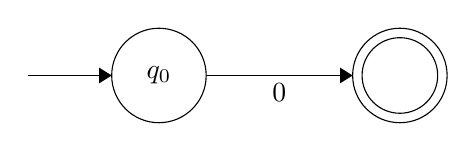
\begin{tikzpicture}[scale=0.2]
              \tikzstyle{every node}+=[inner sep=0pt]
              \draw [black] (29.8,-21.7) circle (3);
              \draw (29.8,-21.7) node {$q_0$};
              \draw [black] (45.1,-21.7) circle (3);
              \draw [black] (45.1,-21.7) circle (2.4);
              \draw [black] (21.5,-21.7) -- (26.8,-21.7);
              \fill [black] (26.8,-21.7) -- (26,-21.2) -- (26,-22.2);
              \draw [black] (32.8,-21.7) -- (42.1,-21.7);
              \fill [black] (42.1,-21.7) -- (41.3,-21.2) -- (41.3,-22.2);
              \draw (37.45,-22.2) node [below] {$0$};
            \end{tikzpicture}
          \end{center}


          Next, we'll create an automaton for matching 1:
          \begin{center}
            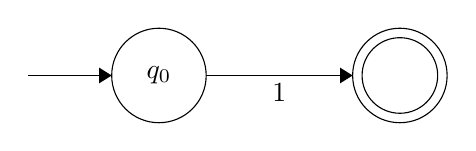
\begin{tikzpicture}[scale=0.2]
              \tikzstyle{every node}+=[inner sep=0pt]
              \draw [black] (29.8,-21.7) circle (3);
              \draw (29.8,-21.7) node {$q_0$};
              \draw [black] (45.1,-21.7) circle (3);
              \draw [black] (45.1,-21.7) circle (2.4);
              \draw [black] (21.5,-21.7) -- (26.8,-21.7);
              \fill [black] (26.8,-21.7) -- (26,-21.2) -- (26,-22.2);
              \draw [black] (32.8,-21.7) -- (42.1,-21.7);
              \fill [black] (42.1,-21.7) -- (41.3,-21.2) -- (41.3,-22.2);
              \draw (37.45,-22.2) node [below] {$1$};
            \end{tikzpicture}
          \end{center}

          Next, we'll combine these two machines to create an automaton that matches $(0 + 1)$:
          \begin{center}
            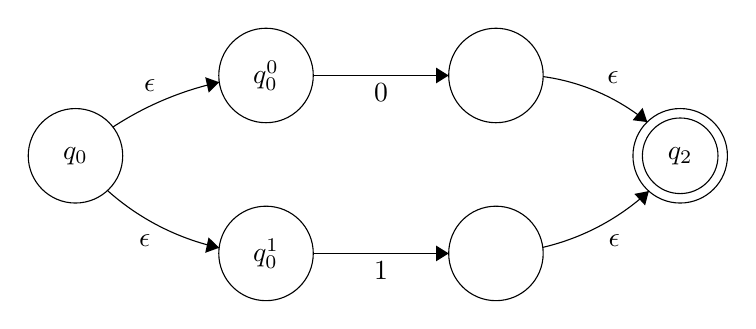
\begin{tikzpicture}[scale=0.2]
              \tikzstyle{every node}+=[inner sep=0pt]
              \draw [black] (32.4,-21.7) circle (3);
              \draw (32.4,-21.7) node {$q_0^0$};
              \draw [black] (47,-21.7) circle (3);
              \draw [black] (32.4,-33) circle (3);
              \draw (32.4,-33) node {$q_0^1$};
              \draw [black] (47,-33) circle (3);
              \draw [black] (20.3,-26.8) circle (3);
              \draw (20.3,-26.8) node {$q_0$};
              \draw [black] (58.7,-26.8) circle (3);
              \draw (58.7,-26.8) node {$q_2$};
              \draw [black] (58.7,-26.8) circle (2.4);
              \draw [black] (35.4,-21.7) -- (44,-21.7);
              \fill [black] (44,-21.7) -- (43.2,-21.2) -- (43.2,-22.2);
              \draw (39.7,-22.2) node [below] {$0$};
              \draw [black] (35.4,-33) -- (44,-33);
              \fill [black] (44,-33) -- (43.2,-32.5) -- (43.2,-33.5);
              \draw (39.7,-33.5) node [below] {$1$};
              \draw [black] (22.678,-24.975) arc (123.26628:102.44336:20.284);
              \fill [black] (29.43,-22.13) -- (28.54,-21.81) -- (28.76,-22.79);
              \draw (25.01,-22.73) node [above] {$\epsilon$};
              \draw [black] (29.426,-32.639) arc (-102.401:-131.8599:15.681);
              \fill [black] (29.43,-32.64) -- (28.75,-31.98) -- (28.54,-32.96);
              \draw (24.7,-31.78) node [below] {$\epsilon$};
              \draw [black] (49.993,-21.77) arc (82.19121:50.70427:13.305);
              \fill [black] (56.61,-24.66) -- (56.31,-23.76) -- (55.68,-24.54);
              \draw (54.43,-22.24) node [above] {$\epsilon$};
              \draw [black] (56.715,-29.042) arc (-47.2781:-76.88237:14.938);
              \fill [black] (56.71,-29.04) -- (55.79,-29.22) -- (56.47,-29.95);
              \draw (54.52,-31.77) node [below] {$\epsilon$};
            \end{tikzpicture}
          \end{center}

          Next, we'll introduce the $\star$. We'll form an automaton that matches $(0 + 1)^\star$.
          \begin{center}
            \begin{tikzpicture}[scale=0.2]
              \tikzstyle{every node}+=[inner sep=0pt]
              \draw [black] (32.4,-21.7) circle (3);
              \draw (32.4,-21.7) node {$q_0^0$};
              \draw [black] (47,-21.7) circle (3);
              \draw [black] (32.4,-33) circle (3);
              \draw (32.4,-33) node {$q_0^1$};
              \draw [black] (47,-33) circle (3);
              \draw [black] (20.3,-26.8) circle (3);
              \draw (20.3,-26.8) node {$q_0'$};
              \draw [black] (58.7,-26.8) circle (3);
              \draw (58.7,-26.8) node {$q_2$};
              \draw [black] (72.4,-26.8) circle (3);
              \draw (72.4,-26.8) node {$q_3$};
              \draw [black] (6.8,-26.8) circle (3);
              \draw (6.8,-26.8) node {$q_0$};
              \draw [black] (35.4,-21.7) -- (44,-21.7);
              \fill [black] (44,-21.7) -- (43.2,-21.2) -- (43.2,-22.2);
              \draw (39.7,-22.2) node [below] {$0$};
              \draw [black] (35.4,-33) -- (44,-33);
              \fill [black] (44,-33) -- (43.2,-32.5) -- (43.2,-33.5);
              \draw (39.7,-33.5) node [below] {$1$};
              \draw [black] (22.678,-24.975) arc (123.26628:102.44336:20.284);
              \fill [black] (29.43,-22.13) -- (28.54,-21.81) -- (28.76,-22.79);
              \draw (25.01,-22.73) node [above] {$\epsilon$};
              \draw [black] (29.426,-32.639) arc (-102.401:-131.8599:15.681);
              \fill [black] (29.43,-32.64) -- (28.75,-31.98) -- (28.54,-32.96);
              \draw (24.7,-31.78) node [below] {$\epsilon$};
              \draw [black] (49.993,-21.77) arc (82.19121:50.70427:13.305);
              \fill [black] (56.61,-24.66) -- (56.31,-23.76) -- (55.68,-24.54);
              \draw (54.43,-22.24) node [above] {$\epsilon$};
              \draw [black] (56.715,-29.042) arc (-47.2781:-76.88237:14.938);
              \fill [black] (56.71,-29.04) -- (55.79,-29.22) -- (56.47,-29.95);
              \draw (54.52,-31.77) node [below] {$\epsilon$};
              \draw [black] (9.8,-26.8) -- (17.3,-26.8);
              \fill [black] (17.3,-26.8) -- (16.5,-26.3) -- (16.5,-27.3);
              \draw (13.55,-27.3) node [below] {$\epsilon$};
              \draw [black] (8.879,-24.638) arc (134.17141:45.82859:44.088);
              \fill [black] (70.32,-24.64) -- (70.1,-23.72) -- (69.4,-24.44);
              \draw (39.6,-11.67) node [above] {$\epsilon$};
              \draw [black] (61.7,-26.8) -- (69.4,-26.8);
              \fill [black] (69.4,-26.8) -- (68.6,-26.3) -- (68.6,-27.3);
              \draw (65.55,-27.3) node [below] {$\epsilon$};
              \draw [black] (58.414,-29.783) arc (-9.95975:-170.04025:19.203);
              \fill [black] (20.59,-29.78) -- (20.23,-30.66) -- (21.22,-30.48);
              \draw (39.5,-46.16) node [below] {$\epsilon$};
            \end{tikzpicture}
          \end{center}

          The rest of this construction is left as an exercise.
        \end{ex}

      \section{Overview of Regular Languages} \lecture{October 3, 2013}
        The following definitions are equivalent:
        \begin{itemize}
          \item $L$ is regular if for some regular expression $r$, $L = L(r)$.
          \item $L$ is regular if there exists some DFA, $A$, such that $L = L(A)$.
          \item $L$ is regular if there exists some NFA, $N$, such that $L = L(N)$.
          \item $L$ is regular if there exists some $\epsilon$-NFA, $N$, such that $L = L(N)$.
        \end{itemize}

        How can we show that some language $L$ is \underline{not} regular? Let's look at an example.
        \begin{ex}
          Let $L_0 = \set{ 0^n1^n : n \in \mathbb{N} }$. We claim that $L_0$ is not a regular language.

          \begin{proof}
            Assume by way of contradiction that $L_0$ is regular. Therefore, it is $L(A)$ for some DFA $A$. Say $A = (\set{0, 1}, Q, q_0, \delta, F)$. Let $k = |Q|$, the number of states in $A$.
            \\ \\
            Consider $w = 0^{k + 2}1^{k + 2}$. Clearly, $w \in L_0$. Notice that there must be some $i < j \le k + 2$ such that $\hat{\delta}(q_0, 0^i) = \hat{\delta}(q_0, 0^j)$, by the pigeonhole principle.
            \\ \\
            \textbf{The Pigeonhole Principle}: if you have more pigeons than holes, then you can't have every pigeon in its hole alone.
            \\ \\
            Note that
            $$
            0^{k + 2}1^{k+2} = \underbrace{0^i 0^{j - i}0^{k + 2 - j}}_{0^{k+2}} 1^{k+2}
            $$

            We can now see that $w' = 0^i 0^{j - i} 0^{j - i} 0^{k + 2 - j}1^{k + 2} \not \in L_0$. The general idea here is that if we take a long enough word, it must visit the same state again, which means we may accept members into our language that aren't supposed to be part of the language.
          \end{proof}
        \end{ex}

      \subsection{The Pumping Lemma}
       \begin{lemma}[The Pumping Lemma]
          For every regular language $L$, there exists some number $n$ such that for every $w \in L$, if $|w| \ge n$, then there are $x, y, z$ so that
          \begin{enumerate}
            \item $xyz = w$,
            \item $|xy| \le n$,
            \item $y \ne \epsilon$, and
            \item For every $k$, $xy^k z \in L$
          \end{enumerate}
        \end{lemma}

        Note that the converse is \emph{not} true. There are languages that are not regular that still satisfy these properties.
        \\ \\
        Let's begin by looking at some positive examples.
        \begin{ex}
          Let $r = (0011)^\star$, and let $L = L(r)$. Pick $n = 5$. For every $w \in L$ such that $|w| > 5$, we have the general form
          $$
            \underbrace{0011}_{y} \underbrace{001100110011}_{z} \ldots
          $$

          Pick $x = \epsilon, y = 0011$, and $z = $ the rest of $w$. Remember: just because a language satisfies these properties, does \emph{not} prove it is regular.
        \end{ex}

        \begin{ex}
          Let $L_{7a} = \set{ w \in \set{a, b}^\star : \text{ the 7th-to-last letter in } w \text{ is a}}$.
          \\ \\
          Let $x$ be the first letter in $w$, and let $y$ be the second letter in $w$. Note that pumping $y$ does not affect the last 7 letters, so the pumped words would still be in the language, as expected.
        \end{ex}

        Now, let's look at a couple of negative examples.
        \begin{ex}
          Let $L_\text{plus} = \set{0^s 1^t 0^r : s + t = r}$.
          \\ \\
          \textbf{Claim}: $L_\text{plus}$ is not regular. This is an intuitive claim since finite automata do not have memory. They only know which state they're currently in. Similarly, counting numbers $> 10$ on your fingers (without using memory) can only determine the count modulus 10, since we only have 10 fingers.
          \\ \\
          We need to show that the claim of the Pumping Lemma fails. Given some $n$, consider
          $$
            w = 0^n 1 0^{n + 1} \in L_\text{plus}
          $$

          For every choice of $x, y, z$, satisfying requirements (1), (2), and (3), inevitably $x = 0^i, y = 0^j$ such that $i+j \le n$ and $j > 0$. Then we have $z = 0^{n - (i + j)} 1 0^{n + 1}$.
          \\ \\
          Pick $k = 2$. Then we have
          \begin{align*}
            xy^kz &= 0^i 0^{2j} 0^{n - (i + j)} 1 0^{n + 1} \\
            &= 0^{n + j} 1 0^{n + 1}
          \end{align*}
          where $j > 0$, which is not in $L_\text{plus}$.
        \end{ex}

        We could rephrase the Pumping Lemma in terms of a game between two players, $R$ and $NR$. $R$ is the player who is trying to convince us that the language is regular, and $NR$ is the player who is trying to convince us otherwise.
        \\ \\
        First, $R$ chooses an $n$. $NR$ can then fire back with a word $w$ such that $w \in L$ and $|w| \ge n$. $R$ can then provide an $x, y, z$ such that $|xy| \le n$, $xyz = w$, and $y \ne \epsilon$.
        \\ \\
        If $xy^kz \in L$ for all $k$, then $R$ wins. If $xy^kz \not \in L$ for some $k$, then $NR$ wins.
        \\ \\
        The Pumping Lemma states that if $L$ is regular, the player $R$ can guarantee that she wins.

        \begin{ex}
          Consider $L_\text{prime} = \set{\underbrace{a \ldots a}_{p \text{ times}} : p \text{ is prime}} = \set{ \underbrace{aa}_{2}, \underbrace{aaa}_3, \underbrace{aaaaa}_5, \underbrace{aaaaaaa}_7, \ldots}$.
          \\ \\
          \textbf{Claim}: $L_\text{prime}$ is not regular.
          \\ \\
          We wish to show that the player $NR$ can defeat the player $R$, regardless of how well $R$ plays the game. Let $n$ be the number picked by the player $R$. Let $p$ be a prime number greater than $n + 2$.
          \\ \\
          Pick $w = a^p \in L_\text{prime}$. Suppose $R$ picks some $xyz$ satisfying requirements (1), (2), and (3). Let $x = a^r, y = a^m$, and $z = a^{p - (r + m)}$ where $m \ge 1$ and $r + m \le n$.
          \\ \\
          Player $NR$ now picks $k = (p - m)$. Then we have
          \begin{align*}
            xy^k z &= a^r a^{m(p-m)} a^{p-(r + m)} \\
            &= a^{m(p-m) + (p-m)}
          \end{align*}

          Note that $(p - m)(m + 1)$ is not prime, because it's two factors, where $p - m > 1$ (since $m < n < p$), and $m + 1 > 1$ (since $m \ge 1$). Therefore, this string cannot have a prime length, so $xy^k z \not \in L_\text{prime}$.
        \end{ex}

        \begin{ex} \lecture{October 8, 2013}
          Let $L_{klk} = \set{ 0^k 1^l 0^k : k, l \in \mathbb{N}}$. Intuitively, this language is not regular because a machine with finite memory cannot remember how many zeros it counted for the first run of 0s.
          \\ \\
          \textbf{Claim}: $L_{klk}$ is not a regular language.

          \begin{proof}
            We will prove this claim with the Pumping Lemma. We need to show that player $NR$ can win, regardless of what player $R$ does.
            \\ \\
            Given some $n$ (chosen by player $R$), our first try is to choose $w = 0^{2n}$. In this case, we may attempt to construct $x = \epsilon, z = \epsilon, y = 0^{2n}$, but that violates the second condition of the Pumping Lemma. We may also try $x = \epsilon, y = 00, z = 0^{2n - 2}$ = the rest of the word. For any $k$ that $NR$ picks, $xy^kz = (00)^k 0^{2n - 2} = 0^{2(k + n - 1)} \in L_{klk}$. $R$ won in this case, which is not what we want. Note that just because $R$ won in this case, does not prove that $L_{klk}$ is regular.
            \\ \\
            Let's try another word. Given some $n$ (chosen by player $R$), we will choose $w = 0^n 1^n 0^n$. Any choice of $x, y$ such that string $|xy| \le n$ will have $z = 0^i 1^n 0^n$. Now pick $k$ arbitrarily; say $k = 2$. Then since $0^j$ for some $j \ge 1$, $xy^2z = 0^{n + j}1^n0^n \not \in L_{klk}$.
          \end{proof}
        \end{ex}

        \begin{ex}
          Let $L_< = \set{w : \#_0(w) > \#_1(w) }$. Intuitively, this language is non-regular because we can't check this condition with unbounded memory. In some \emph{particular} cases, such as $w = 0101010101$, we \emph{can} verify membership with bounded memory. Such words would not be good candidates for $w$ in our proof.
          \\ \\
          \textbf{Claim}: $L_<$ is not regular.

          \begin{proof}
            We will prove this claim with the Pumping Lemma. We need to show that player $NR$ always wins.
            \\ \\
            Given some $n$, pick $w = 1^n 0^{n + 1}$. Now, since $|xy| \le n$, player $R$ is forced to choose $x = 1^j, y = 1^i, z = 1^{n - (i + j)} 0^{n + 1}$, for $i \ge 1$. Any $k > 1$ will then result in $xy^kz \not \in L_<$.
          \end{proof}
        \end{ex}

        \textbf{Claim}: let $L$ be a non-empty language that for some $s \in \mathbb{N}$ accepts no words of length $\le s$. Then, if a DFA $A$ computes $L$ (that is, $L = L(A)$), then inevitably, $A$ has more than $s$ states.
        \\ \\
        For example, $L_{> 6} = \set{ w : |w| > 6 }$ is not $L(A)$ for any DFA with at most 6 states.
        \\ \\
        Note that languages of this form \emph{are} regular. We only need to count up to $s$, which would require $s$ states. For instance, $L_{> 6}$ is regular because the following DFA computes it:
        \begin{center}
          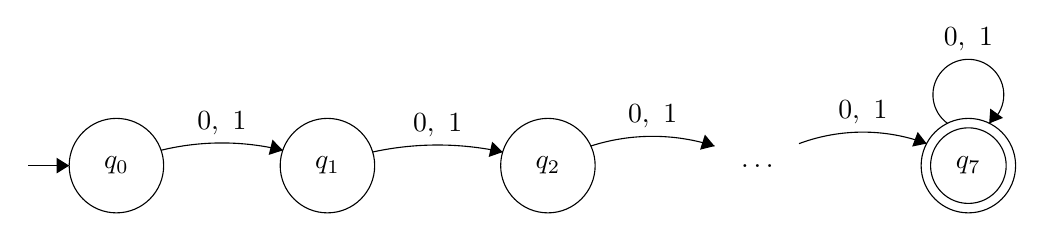
\begin{tikzpicture}[scale=0.2]
            \tikzstyle{every node}+=[inner sep=0pt]
            \draw [black] (20.2,-26.8) circle (3);
            \draw (20.2,-26.8) node {$q_1$};
            \draw [black] (6.8,-26.8) circle (3);
            \draw (6.8,-26.8) node {$q_0$};
            \draw [black] (34.2,-26.8) circle (3);
            \draw (34.2,-26.8) node {$q_2$};
            \draw (47.5,-26.8) node {$\ldots$};
            \draw [black] (60.9,-26.8) circle (3);
            \draw (60.9,-26.8) node {$q_7$};
            \draw [black] (60.9,-26.8) circle (2.4);
            \draw [black] (9.633,-25.825) arc (103.71876:76.28124:16.307);
            \fill [black] (17.37,-25.83) -- (16.71,-25.15) -- (16.47,-26.12);
            \draw (13.5,-24.86) node [above] {$0,\mbox{ }1$};
            \draw [black] (23.07,-25.936) arc (102.31525:77.68475:19.364);
            \fill [black] (31.33,-25.94) -- (30.66,-25.28) -- (30.44,-26.25);
            \draw (27.2,-24.99) node [above] {$0,\mbox{ }1$};
            \draw [black] (36.922,-25.556) arc (107.85352:72.14648:12.811);
            \fill [black] (44.78,-25.56) -- (44.17,-24.83) -- (43.86,-25.79);
            \draw (40.85,-24.44) node [above] {$0,\mbox{ }1$};
            \draw [black] (50.146,-25.403) arc (110.43363:69.56637:11.613);
            \fill [black] (58.25,-25.4) -- (57.68,-24.66) -- (57.33,-25.59);
            \draw (54.2,-24.17) node [above] {$0,\mbox{ }1$};
            \draw [black] (59.577,-24.12) arc (234:-54:2.25);
            \draw (60.9,-19.55) node [above] {$0,\mbox{ }1$};
            \fill [black] (62.22,-24.12) -- (63.1,-23.77) -- (62.29,-23.18);
            \draw [black] (1.2,-26.8) -- (3.8,-26.8);
            \fill [black] (3.8,-26.8) -- (3,-26.3) -- (3,-27.3);
          \end{tikzpicture}
        \end{center}

        \begin{proof}
          Note that if $L = L(A)$ for some DFA $A$, then in the Pumping Lemma, one can pick $n = |Q^A|$ (the number of states in $A$).
          \\ \\
          Assume by way of contradiction that for some $A$ with $n < s$ states, $L = L(A)$. Apply the Pumping Lemma where player $R$ chooses $n = |Q^A|$. Let $w$ be a word of shortest length in $L$. Note that $|w| > s > n$, which makes this a legal choice.
          \\ \\
          Given a decomposition $x, y, z$, choose $k = 0$. Since $xyz = w,~ |xy^0z| < |w|$. This is a contradiction since we assumed we selected the smallest word in $L$, and then we made it shorter.
        \end{proof}

      \subsection{Equivalent Descriptions of Languages}
        Earlier in the course, we stated a basic theorem that we didn't prove fully. We'd like to complete that proof now.

        \begin{theorem}
          The following conditions on a language are equivalent:
          \begin{enumerate}
            \item $L = L(r)$ for some regular expression $r$.
            \item $L = L(A)$ for some DFA $A$.
            \item $L = L(N)$ for some NFA $N$.
            \item $L = L(N)$ for some $\epsilon$-NFA $N$.
          \end{enumerate}
        \end{theorem}

        We've shown $(1) \implies (2)$ and $(3) \implies (2)$ in class previously. $(2) \implies (3) \implies (4)$ is trivial. We're still missing $(2) \implies (1)$, so we'll prove that now.

        \begin{lemma}
          For every DFA, $A$, there exists a regular expression $r$, such that $L(r) = L(A)$.
        \end{lemma}

        \begin{proof}
          Let $A = (\Sigma, Q, q_0, \delta, F)$. Without loss of generality, redefine $Q = \set{ q_1, \ldots, q_n }$ for some $n$.
          \\ \\
          By induction on $k$, we will show that for every $i, j \le n$, there exists a regular expression $R_{ij}^k$ such that $L(R_{ij}^k) = \set{ w : \text{ on } A,~ w \text{ takes us from } q_i \text{ to } q_j \text{ without visiting any state of index } > k}$.
          \\ \\
          Note that
          $$
            L(A) = \bigcup_{q_j \in F} L(R_{ij}^n)
          $$

          \textbf{Base case}: $k = 0$. $L_{ij}^0 = \set{ w : \text{ go from } q_i \text{ to } q_j \text{ without touching any other state}}$. We have two cases.

          \begin{enumerate}
            \item $i \ne j$. If there is an edge between the two states, let $a_1, \ldots, a_k$ be all letters on this edge, and $R_{ij}^0 = a_1 + \ldots + a_k$. If there is no direct edge from $q_i$ to $q_j$, then $R_{ij}^0 = \emptyset$ (i.e. there is no way to go from $q_i$ to $q_j$ without touching any other state).
            \item $i = j$. If there is a self-edge labeled $a_1, \ldots, a_k$, then $R_{ii}^0 = a_1 + \ldots + a_k + \epsilon$. Note that $\epsilon$ is added here because you can also go from a state to itself without reading any letters. If there is no self loop on $q_i$, then $R_{ii}^0 = \epsilon$.
          \end{enumerate}

          \textbf{Induction step}: assume we have regular expressions $R_{ij}^l$ for $i, j \le n$, and $l < k$. Construct $R_{ij}^k$ for all such $i, j$. We then have:
          $$
            R_{ij}^k = R_{ik}^{k - 1} (R_{kk}^{k - 1})^\star R_{kj}^{k - 1} + R_{ij}^{k - 1}
          $$

          $R_{ik}^{k - 1}$ and $R_{kj}^{k - 1}$ indicate the cases where we aren't stepping on state $k$. $(R_{kk}^{k - 1})^\star$ indicates that we can step on state $k$ as many times as we want (or not at all). Finally, $R_{ij}^{k - 1}$ represents the case where we go from state $q_i$ to $q_j$ without stepping on $q_k$ at all.
        \end{proof}

      \subsection{Algorithms on Languages and Finite Automata} \lecture{October 10, 2013}
        Let's look at a number of algorithms that you should be able to carry out on languages and automata.

        \begin{enumerate}
          \item \textbf{Given $\boldsymbol{w}$ and DFA (or NFA, or $\boldsymbol{\epsilon}$-NFA) $\boldsymbol{M}$, decide if $\boldsymbol{w \in L(M)}$.}
          \item \textbf{Given a regular expression $\boldsymbol{r}$, construct a ($\boldsymbol{\epsilon}$-)NFA, $\boldsymbol{M}$, such that $\boldsymbol{L(M) = L(r)}$.}
          \begin{ex}
            Let $r = (a + b) a^\star + b(a + \epsilon)$.
            \\ \\
            Start by constructing an automaton for atoms $a, b$, and $\epsilon$, then move on to more complex expressions like $(a + b)$ or $(a + \epsilon)$ by combining the automata created previously.
          \end{ex}

          \item \textbf{Given $\boldsymbol{w}$ and $\boldsymbol{r}$, is $\boldsymbol{w \in L(r)}$?} Note that this is difficult to do in general without converting the regular expression to an automaton.

          \item \textbf{Given an NFA, $\boldsymbol{M}$, construct a DFA $\boldsymbol{A}$ such that $\boldsymbol{L(M) = L(A)}$.} Recall that states in the equivalent DFA each represent a set of states from the NFA.

          \item \textbf{Given a DFA, $\boldsymbol{A}$, construct a regular expression $\boldsymbol{r}$ such that $\boldsymbol{L(r) = L(A)}$.} We briefly touched on this before, so we'll do a more in-depth example now.
          \\ \\
          \textbf{General idea}:
          \begin{enumerate}
            \item Rename the states of $A$ as $\set{ q_1, \ldots, q_n }$ for some $n$.
            \item For every $k, i, j \le n$, let $R_{ij}^k = $\{$w$ : if we read $w$ starting in state $i$, we will end in state $j$, and, along the path, we step on no state whose index is $> k$\}.
            \item By induction on $k$, construct regular expressions $r_{ij}^k$ such that $L(r_{ij}^k) = R_{ij}^k$ (for all $i, j$)
            \item Finally, to get a regular expression for $L(A)$, let $r = \sum \{ r_{ij}^n : i \in F \}$.
          \end{enumerate}

          \begin{ex}
            Let $A$ be the following DFA:
            \begin{center}
              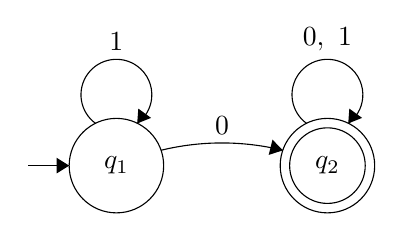
\begin{tikzpicture}[scale=0.2]
                \tikzstyle{every node}+=[inner sep=0pt]
                \draw [black] (20.2,-26.8) circle (3);
                \draw (20.2,-26.8) node {$q_2$};
                \draw [black] (20.2,-26.8) circle (2.4);
                \draw [black] (6.8,-26.8) circle (3);
                \draw (6.8,-26.8) node {$q_1$};
                \draw [black] (9.633,-25.825) arc (103.71876:76.28124:16.307);
                \fill [black] (17.37,-25.83) -- (16.71,-25.15) -- (16.47,-26.12);
                \draw (13.5,-24.86) node [above] {$0$};
                \draw [black] (1.2,-26.8) -- (3.8,-26.8);
                \fill [black] (3.8,-26.8) -- (3,-26.3) -- (3,-27.3);
                \draw [black] (18.877,-24.12) arc (234:-54:2.25);
                \draw (20.2,-19.55) node [above] {$0,\mbox{ }1$};
                \fill [black] (21.52,-24.12) -- (22.4,-23.77) -- (21.59,-23.18);
                \draw [black] (5.477,-24.12) arc (234:-54:2.25);
                \draw (6.8,-19.55) node [above] {$1$};
                \fill [black] (8.12,-24.12) -- (9,-23.77) -- (8.19,-23.18);
              \end{tikzpicture}
            \end{center}

            Notice that $L(A) = \set{ w : w \text{ contains a } 0}$. We can also see that a regular expression for this language is $r = 1^\star 0(0 + 1)^\star$, but determining this was only possible because this automaton is simple.
            \\ \\
            If we couldn't determine the regular expression like this, we could alternatively follow the translation procedure. The translation procedure requires much more work, but no creativity or luck is necessary.
            \\ \\
            We need the following tables in order to carry out the translation procedure:
            \begin{center}
              \begin{tabular}{c|c}
                0 & regular expression \\ \hline
                $R_{11}^0$ & $(1 + \epsilon)$ \\
                $R_{12}^0$ & $0$ \\
                $R_{21}^0$ & $\emptyset$ \\
                $R_{22}^0$ & $0 + 1 + \epsilon$
              \end{tabular}
              \begin{tabular}{c|c}
                1 & regular expression \\ \hline
                $R_{11}^1$ & $r_{11}^0 (r_{11}^0)^\star r_{11}^0 + r_{11}^0$ \\
                $R_{12}^1$ & $r_{11}^0  (r_{11}^0)^\star r_{12}^0 + r_{12}^0$ \\
                $R_{21}^1$ & \\
                $R_{22}^1$ & \\
              \end{tabular}
              \begin{tabular}{c|c}
                2 & regular expression \\ \hline
                $R_{11}^0$ & \\
                $R_{12}^0$ & \\
                $R_{21}^0$ & \\
                $R_{22}^0$ & \\
              \end{tabular}
            \end{center}

            The 0, 1, and 2 in the headers of these tables represent the superscript. You need to fill out these tables fully, although we have omitted some of that here.
            \\ \\
            How do we construct $r_{ij}^k$ from the expressions $\set{ r_{ij}^{k - 1} : i, j \le m }$? You can use the recursive formula:
            $$
              r_{ij}^k = r_{ik}^{k - 1} (r_{kk}^{k - 1})^\star r_{kj}^{k - 1} + r_{ij}^{k - 1}
            $$

            Here's a visualization:
            \begin{center}
              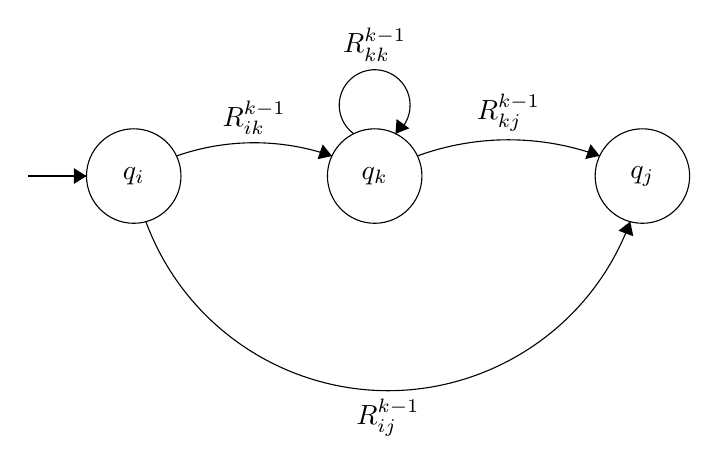
\begin{tikzpicture}[scale=0.2]
                \tikzstyle{every node}+=[inner sep=0pt]
                \draw [black] (10.8,-26.6) circle (3);
                \draw (10.8,-26.6) node {$q_i$};
                \draw [black] (26.1,-26.6) circle (3);
                \draw (26.1,-26.6) node {$q_k$};
                \draw [black] (43.1,-26.6) circle (3);
                \draw (43.1,-26.6) node {$q_j$};
                \draw [black] (4.1,-26.6) -- (7.8,-26.6);
                \fill [black] (7.8,-26.6) -- (7,-26.1) -- (7,-27.1);
                \draw [black] (13.511,-25.328) arc (109.35982:70.64018:14.898);
                \fill [black] (23.39,-25.33) -- (22.8,-24.59) -- (22.47,-25.53);
                \draw (18.45,-23.99) node [above] {$R_{ik}^{k-1}$};
                \draw [black] (28.811,-25.324) arc (110.10822:69.89178:16.84);
                \fill [black] (40.39,-25.32) -- (39.81,-24.58) -- (39.47,-25.52);
                \draw (34.6,-23.8) node [above] {$R_{kj}^{k-1}$};
                \draw [black] (24.777,-23.92) arc (234:-54:2.25);
                \draw (26.1,-19.35) node [above] {$R_{kk}^{k-1}$};
                \fill [black] (27.42,-23.92) -- (28.3,-23.57) -- (27.49,-22.98);
                \draw [black] (42.328,-29.495) arc (-20.18023:-159.81977:16.384);
                \fill [black] (42.33,-29.49) -- (41.58,-30.07) -- (42.52,-30.42);
                \draw (26.95,-40.73) node [below] {$R_{ij}^{k-1}$};
              \end{tikzpicture}
            \end{center}
          \end{ex}


          \item \textbf{Given a DFA $\boldsymbol{A = (\Sigma, Q, q_0, \delta, F)}$, decide whether $\boldsymbol{L(A) = \emptyset}$ or not.}
          \\ \\
          We can't just use a regular expression representation of $A$ to determine this, since $L(\emptyset) = \emptyset$, but there are also other regular expressions $r$ such that $L(r) = \emptyset$. For example, $\emptyset + \emptyset$, $(\emptyset + \emptyset)(\emptyset + \emptyset)$, or $((a + b)b^\star + b)\emptyset$.
          \\ \\
          \underline{Algorithm 1}: recall that if $L(A)$ contains no strings of length $\le |Q|$ then $L(A) = \emptyset$, by the Pumping Lemma.
          \\ \\
          Now, list all strings of length $\le |Q|$: say, $w_0, w_1, \ldots, w_{2^{|Q|}}$. For each such $w_i$, check whether $w_i \in L(A)$. If all these words are rejected, then we can conclude that $L(A)$ is empty.
          \\ \\
          \underline{Algorithm 2}: check if there's a path that starts in $q_0$ and ends in an accepting state. This uses the concept of \textbf{reachability}. Construct:
          \begin{align*}
            \set{q_0} &= \text{ all states reachable from } q_0 \text{ with 0 edges} \\
            \vdots & \\
            A_k &= \text{ all states reachable from } q_0 \text{ traversing at most } k \text{ edges} \\
            A_{k + 1} &= A_k \cup \set{ \text{all neighbors}}
          \end{align*}

          Finally, check $A_n \cap F$. If this set is empty, then $L(A) = \emptyset$. Otherwise, a path exists which means $L(A)$ is non-empty.

          \item \textbf{Given two DFAs, $\boldsymbol{A_1, A_2}$, decide whether $\boldsymbol{L(A_1) = L(A_2)}$.} Note that these languages could be arbitrarily large. Also, keep in mind that there could be different regular expressions, graphs, and automata that all compute the same language.
          \\ \\
          \textbf{Claim}: $L(A_1) = L(A_2)$ if and only if $L(A_1) \backslash L(A_2) = \emptyset$ and $L(A_2) \backslash L(A_1) = \emptyset$.
          \\ \\
          We need to construct $A_3$ such that $L(A_3) = L(A_1) \backslash L(A_2)$ (using the product automaton). Similarly, we need to construct $A_4$ such that $L(A_4) = L(A_2) \backslash L(A_1)$.
          \\ \\
          We then check for emptiness in both $L(A_3)$ and $L(A_4)$. If both are empty, then we can conclude that $L(A_1) = L(A_2)$. Otherwise, $L(A_1) \ne L(A_2)$.
          \\ \\
          Recall that if $A_1 = (\Sigma, Q^1, q_0^1, \delta^1, F^1), A_2 = (\Sigma, Q^2, q_0^2, \delta^2, F^2)$, then $A_3 = (\Sigma, Q^1 \times Q^2, (q_0^1, q_0^2), \delta^1 \times \delta^2, \set{ (q, p) : q \in F_1, p \not \in F_2 })$. The construction of $A_4$ is similar.
          \\ \\
          Alternatively, we could check all strings of length at most $|Q^1| \cdot |Q^2|$. If the machines agree on all of those strings, then they will always agree and are therefore equivalent machines.

          \item \textbf{Given a DFA $\boldsymbol{A}$, decide whether $\boldsymbol{L(A)}$ is infinite.}
          \\ \\
          A possible algorithm for this is to check the graph, looking for cycles that are reachable from $q_0$ and can eventually reach an accepting state.
          \\ \\
          \textbf{Claim}: let $A = (\Sigma, Q, q_0, \delta, F)$. $L(A)$ is finite if and only if it contains no $w$ of length $|Q| < |w| \le 2|Q|$.
          \\ \\
          The Pumping Lemma could be used to prove this claim.
        \end{enumerate}

  \section{Context-Free Grammars} \lecture{October 15, 2013}
    There are some languages that are more complex than regular languages. Let's look at a few examples of such languages.

    \begin{ex}
      Let $\Sigma = \set{a, b, +, (, )}$. Let $L = \{w  \in \Sigma^\star : w $ has the same number of left brackets as right brackets\}.
      \\ \\
      \textbf{Claim}: $L$ is not a regular language. This is intuitively clear because a finite amount of memory cannot be used to count the number of left parentheses to compare to the number of right parentheses.

      \begin{proof}
        Apply the Pumping Lemma to expressions of the form
        $$
          \underbrace{((((}_{n} \underbrace{))))}_{n}
        $$
      \end{proof}
    \end{ex}

    \begin{ex}
      Let $\Sigma = \set{0, 1}$ and $L_p = \{w \in \set{0, 1}^\star : w $ is a palindrome\}. Namely, $w = w^R$ ($w$ is equal to $w$ reversed). For example, ``MALAYALAM'' and ``MADAM'' are palindromes.
      \\ \\
      \textbf{Claim}: $L_p$ is not a regular language.

      \begin{proof}
        We will apply the Pumping Lemma. Given $n$, consider $w = 0^n 1 0^n \in L_p$. Note that $|w| \ge n$ and $xyz$ exist such that $|xy| \le n$, so $xy = 0^k$ for some $k \le n$. So, $xy^2z = 0^m 1 0^n$ for some $m > n$, so $w \not \in L_p$.
      \end{proof}
    \end{ex}

    We will introduce the notion of a \textbf{context-free grammar} (\textbf{CFG}). A CFG is a set of rules of a particular form for defining languages.

    \begin{ex}
      Let's consider $L_p$ again -- the language of all $\set{0, 1}$-palindromes. A context-free grammar for this language could have the following rules:
      \begin{align}
        S& \\
        S &\to 0 \\
        S &\to 1 \\
        S &\to \epsilon \\
        S &\to 0S0 \\
        S &\to 1S1
      \end{align}
      \setcounter{equation}{0}

      An example construction of the palindrome ``011110'' is as follows:

      \begin{align*}
        S &\text{ by (1)} \\
        0S0 &\text{ by (5)} \\
        01S10 &\text{ by (6)} \\
        011S110 &\text{ by (6)} \\
        011110 &\text{ by (4)}
      \end{align*}

      \textbf{Claim}: the set of words in $\set{0, 1}^\star$ that can be obtained by starting with $S$ and applying the rules a finite number of times equals the set of all palindromes over $\set{0, 1}^\star$.
      \\ \\
      In order to prove this claim, we must prove two separate claims:
      \begin{enumerate}
        \item Every word that these rules generate is of the form $wSw^R$ or $w0w^R$ or $w1w^R$ or $ww^R$, for some $w \in \set{0, 1}^\star$.
        \\ \\
        The set of all expressions that can be generated by these rules is $I(A, P)$ for $A = \set{S}$, and $P = \set{ S \to 0, S \to 1, S \to \epsilon, S \to 0S0, S \to 1S1}$. Therefore, we can prove this claim by structural induction.
        \item These rules will generate \underline{all} palindromes.
        \\ \\
        This claim could also be proven by structural induction. Let $A = \set{\epsilon, 0, 1}$, and let $P = \set{ \AxiomC{w} \UnaryInfC{0w0} \DisplayProof, \AxiomC{w} \UnaryInfC{1w1} \DisplayProof }$. Then, $L_p = I(A, P)$.
      \end{enumerate}
    \end{ex}

    \subsection{Defining Context-Free Grammars}
      \begin{defn}
        A \textbf{context-free grammar} (or \textbf{CFG}) is a tuple $G = (V, T, P, S)$, where
        \begin{itemize}
          \item $V$ is a finite set of variables.
          \item $T$ is a finite set of terminal symbols, disjoint from $V$.
          \item $P$ is a finite set of rules. Each rule of $P$ has the form $X \to \sigma$, where $X \in V$ and $\sigma \in (V \cup T)^\star$.
          \item $S \in V$ is the start symbol.
        \end{itemize}
      \end{defn}

      In the example of generating palindromes, $V = \set{S},~ T = \set{0, 1},~ S = S$, and $P = \set{S \to \epsilon, S \to 0, S \to 1, S \to 0S0, S \to 1S1 }$.
      \\ \\
      You might be wondering why we call these languages ``context-free.'' The rules in a CFG can only consider the variable at hand -- not the context of its neighbours in a larger string. Context-free grammars are limited by requiring that a variable generates the same expression regardless of the word the variable is embedded in.

      \subsubsection{Defining The Languages Generated By Such Grammars}
        Given a CFG $G = (V, T, P, S)$, we wish to define $L(G)$, the language described by $G$. But first, we have a couple of preliminary technical definitions of some notation.

        \begin{defn}
          For a variable $X \in V$ and some $\sigma \in (V \cup T)^\star$, we say that $X \underset{G}{\overset{\star}{\implies}} \sigma$ if $\sigma$ can be obtained from $X$ by applying a finite sequence of rules from $P$ of $G$.
        \end{defn}

        For instance, in the grammar for $L_p$, we can say $S \underset{G}{\overset{\star}{\implies}} 0$, $S \underset{G}{\overset{\star}{\implies}} 0S0$, $S \underset{G}{\overset{\star}{\implies}} 01S10$, etc.

        \begin{defn}
          $r \underset{G}{\overset{n}{\implies}} u$ denotes that $r$ entails $u$ in $n$ steps. $r \underset{G}{\overset{1}{\implies}} u$ if and only if $r = u$. By induction, we say $r \underset{G}{\overset{n+1}{\implies}} u$ if and only if for some $v$, $r \underset{G}{\overset{n}{\implies}} v$ and $v \underset{G}{\overset{1}{\implies}} u$.
        \end{defn}

        This leads to a reworded definition of $r \underset{G}{\overset{\star}{\implies}} u$.
        \begin{defn}
          $r \underset{G}{\overset{\star}{\implies}} u$ if and only if for some $n$, $r \underset{G}{\overset{n}{\implies}} u$.
        \end{defn}

        That's enough technical definitions. Let's now define the language described by a context-free grammar, $G$.

        \begin{defn}
          $L(G)$, the language described by $G$, is defined as
          $$
            L(G) := \set{ w \in T^\star : S \underset{G}{\overset{\star}{\implies}} w}
          $$
        \end{defn}

        Note that the words $w$ included in the language $L(G)$ do not contain any variables -- only terminal symbols.

        \begin{ex}
          Let $L_< = \set{0^m 1^k : m \le k}$. Note that $L_<$ is clearly not a regular language. So, we wish to define $G = (V, T, P, S)$ to describe $L_<$. Let's look at two different ways of defining this grammar.
          \\ \\
          Our first grammar for $L_<$ is:
          \begin{itemize}
            \item $V = \set{S}$
            \item $T = \set{0, 1}$
            \item $P = \set{ S \mapsto \epsilon, S \mapsto 0S1, S \mapsto S1}$
            \item $S = S$
          \end{itemize}

          Note that including $S \mapsto 1$ in $P$ would be redundant because we could use our last rule, $S \mapsto S1$, in conjunction with our first rule, $S \mapsto \epsilon$.
          \\ \\
          Let's now look at another grammar that describes the same language:
          \begin{itemize}
            \item $V = \set{S, A, B}$
            \item $T = \set{0, 1}$
            \item $P = \set{S \mapsto \epsilon, S \mapsto ASB, A \mapsto 0, A \mapsto \epsilon, B \mapsto 1}$
            \item $S = S$
          \end{itemize}

          With this grammar, we always generate a string in the form
          $$
            \underbrace{AAA}_{n} S \underbrace{BBB}_{n}
          $$

          However, some of those $A$s will map to $\epsilon$, effectively eliminating them.
        \end{ex}

    \subsection{Parse Trees}
      \begin{defn}
        A parse tree for a grammar $G = (V, T, P, S)$ is a tree where
        \begin{itemize}
          \item Each vertex is labeled by a member of $V$,
          \item The root is labeled $S$, and,
          \item For every internal node, the set of its immediate children read (from left-to-right) $\sigma$, for $\sigma$ such that $X \to \sigma \in P$, where $X$ is the label of the parent node.
        \end{itemize}
      \end{defn}

      % Note that any subtree of a parse tree is \emph{also} a valid parse tree. In particular, parse trees that don't resolve to legitimate words in the language are still considered valid parse trees.

      \begin{defn}
        Given a parse tree $G$ for some grammar $G$, the \textbf{sentential} described by $T$ is the sequence $\sigma$ of its leaf nodes, read from left-to-right.
      \end{defn}

      We distinguish between sententials and words because a sentential is a sequence that \emph{may} contain variables, and valid words cannot contain variables.

      \begin{ex}
        Consider the previous grammar we described. Let's look at a parse tree for $w = 011$ under this grammar.

        \begin{figure}[H]
          \Tree [.$S$ [.$A$ [.0 ] ] [.$S$ [.$A$ [.$\epsilon$ ] ] [.$S$ [.$\epsilon$ ] ] [.$B$ [.1 ] ] ] [.$B$ [.1 ] ] ]
        \end{figure}
      \end{ex}

      \begin{theorem}
        $\sigma \in (V \cup T)^\star$ has a parse tree with respect to some grammar $G$ if and only if $S \underset{G}{\overset{\star}{\implies}} \sigma$.
      \end{theorem}

      \begin{proof}
        We need to prove two claims to show that this theorem indeed holds.
        \begin{enumerate}
          \item If $S \underset{G}{\overset{\star}{\implies}} \sigma$, then $\sigma$ has a parse tree with respect to $G$.

          \begin{proof}
            We will use structural induction on the generation of $\sigma$.
            \\ \\
            \textbf{Base case}: If $\sigma = S$, then the parse tree is just ``S'' (with no children).
            \\ \\
            \textbf{Induction step}: note that $S \to \sigma_1 \to \sigma_2 \to \ldots \to \sigma$. Assume $\sigma$ was generated by applying a rule from $P$ to a variable in $\sigma'$.
            \\ \\
            By the induction hypothesis, there exists a parse tree $T'$ for $\sigma'$. Since $\sigma$ was generated by applying some rule $X \to \tau$ in $G$, we can append the sequence $\tau$ as children to the node corresponding to $X$ in $T'$, and the new tree, $T$, is a tree for $\sigma$.
          \end{proof}

          \item If $\sigma \in (V \cup T)^\star$ has a parse tree with respect to $G$, then $S \underset{G}{\overset{\star}{\implies}} \sigma$.

          \begin{proof}
            We can prove this claim by induction on the depth of $T$. (The depth of a tree is the number of nodes in the longest path from the root to a leaf.)
            \\ \\
            This proof is left as an exercise.
          \end{proof}
        \end{enumerate}
      \end{proof}

      \lecture{October 17, 2013}
      Parse trees do not concern themselves with the order of application of the rules at each step. However, they do let you see the history of how the rules were applied to each part to derive a particular string (by looking at the levels of the tree above the leaves).

      \begin{corollary}
        $w \in L(G)$ if and only if there exists a parse tree for $G$ whose leaves are labelled by the symbols of $w$.
      \end{corollary}

      \begin{ex}
        We want a grammar to represent propositional logic over the variables $p$ and $q$. For example, $p \vee q$ and $((q \vee (p \to q)) \vee p)$. We will define our grammar as $G = (V, T, P, S)$ where
        \begin{itemize}
          \item $V = \set{S}$
          \item $T = \set{p, q, \to, \vee, \wedge, \neg, (, )}$
          \item $P = \set{S \vdash p,~ S \vdash q,~ S \vdash (S \to S),~ S \vdash (S \vee S),~ S \vdash (S \wedge S),~ (\neg S)}$
          \item $S = S$
        \end{itemize}

        Let's look at a sample parse tree for $((q \vee (p \to q)) \vee p)$:

        \begin{figure}[H]
          \tikzset{sibling distance=15pt}
          \Tree [.$S$ [.$($ ] [.$S$ [.$($ ] [.$S$ [.$q$ ]] [.$\vee$ ] [.$S$ [.$($ ] [.$S$ [.$p$ ]] [.$\to$ ] [.$S$ [.$q$ ]] [.$)$ ] ] [.$)$ ]] [.$\vee$ ] [.$S$ [.$p$ ] ] [.$)$ ] ]
        \end{figure}
      \end{ex}

      Given a grammar $G$, we have a way of verifying that some $w \in L(G)$, by constructing a generating sequence or a parse tree for $w$. We do not have a way of checking if a given $w$ is in $L(G)$ or not. We also don't have a tool for proving that some $w \not \in L(G)$. Finally, we have no way of showing that some language $L$ is \emph{not} context-free.
      \\ \\
      These are some languages that are context-free:
      \begin{itemize}
        \item $\set{ 0^n 1^n : n \in \mathbb{N} }$
        \item $\set{ 0^n 1 0^n : n \in \mathbb{N} }$
        \item $\set{ w : \#_1(w) = \#_0(w) }$
        \item \{$w$ : $w$ is of the form $w' w'^R$ for some $w'$\}
      \end{itemize}

      However, \{$w$ : $w$ is of the form $w' w'$ for some $w'$ \} is \emph{not} a context-free language.

    \subsection{Pushdown Automata}
      The machines corresponding to context-free languages are called \textbf{pushdown automata} (also referred to as \textbf{PDA}s). They are finite automata but with stack memory.
      \\ \\
      Intuitively, it is trivial for a pushdown automaton to compute a language of words like $w = w' w'^R$. You can form a non-deterministic machine that pushes each letter it reads onto the stack, while simultaneously guessing that the top of the stack currently represents the center character of the string. We don't know where the center of the string is, but the nondeterminism will eventually ``guess'' the center correctly. Before we reach the center of the string, we want to push each character we read onto the stack. After the center, we want to compare the next character of the input with the top of the stack. If they're equal, continue, otherwise lead to a blackhole state.
      \\ \\
      These machines make it obvious that a language of all words of the form $w'w'$ cannot possibly be context-free.
      \\ \\
      Creating a machine with stack memory seems arbitrary. However, it's equally arbitrary as the definition of context-free languages. Every context-free language can be computed by a pushdown automaton.
      \\ \\
      Let's discuss pushdown automata more formally.

      \begin{defn}
        A \textbf{pushdown automaton} (\textbf{PDA}) is a tuple $D = (\Sigma, \Gamma, Q, q_0, z_0, \delta, F)$, where
        \begin{itemize}
          \item $\Sigma$ is the alphabet of the language we want to accept.
          \item $\Gamma$ is the set of characters we could store in memory (on the stack) -- and this isn't necessarily equal to $\Sigma$.
          \item $Q$ is the set of states.
          \item $q_0$ is the start state.
          \item $z_0 \in \Gamma$ is the initial content of the stack (in order for us to be able to tell when we've reached the bottom of the stack).
          \item $\delta$ is a set of rules, of the form $(p, a, z) \to (q, \gamma)$, where $\gamma \in \Gamma^\star$. In particular, $p$ is the current state, $a$ is the character read from the input, $z$ is the letter at the top of the stack, and $q$ is the destination state.
          \item $F \subseteq Q$ is the set of accepting states.
        \end{itemize}
      \end{defn}

      $\Gamma$ and $z_0$ are new to us, and the meaning of $\delta$ is different than before. This definition of $\delta$ means ``if you are in state $p$, you see $z$ at the top of the stack, and read input letter $a$, then move to state $q$, and replace $z$ by $\gamma$ at the top of the stack.''
      \\ \\
      What is $L(D)$ for such a machine $D$? Intuitively, it's the set of all words $w$ that can lead from $(q_0, z_0)$ to some accepting state.

      \begin{defn}
        $(p, \gamma, w)$ is an \textbf{instantaneous description} (\textbf{ID}), meaning at this point we are in state $p$, we have $\gamma$ in the stack, and ahead of us, the input is $w$.
      \end{defn}

      \lecture{October 22, 2013}
        \emph{The lecture from October 22, 2013 is omitted. If you have notes from this lecture, feel free to email me (\href{mailto:chris@cthomson.ca}{chris@cthomson.ca}) and I'll include them here.}

        \begin{ex} \lecture{October 24, 2013}
          Consider $L = \set{a^n b^n : n \in \mathbb{N}}$. The context-free grammar for $L$ would have rules $S \to aSb$ and $S \to \epsilon$.
          \\ \\
          The corresponding machine that could accept this language $L$ is a pushdown automaton with these transitions:
          \begin{align*}
            \delta(q_0, a, z_0) &= (q_1, A) \\
            \delta(q_1, a, A) &= (q_1, AA)
          \end{align*}
        \end{ex}

        We aim to show three things:
        \begin{itemize}
          \item The equivalence of a context-free grammar (CFG) to a pushdown automaton (PDA).
          \item A Pumping Lemma for context-free languages.
          \item Closure properties of context-free languages.
        \end{itemize}

        Last time, we considered two ways of defining the language of a pushdown automaton:
        \begin{itemize}
          \item $L_E(D)$, with the emptying of the stack leading to acceptance.
          \item $L_f(D)$, with finite acceptance states.
        \end{itemize}

        Last time, we showed that for every PDA $D_1$, there exists a PDA $D_2$ such that $L_f(D_1) = L_E(D_2)$.
        \\ \\
        \textbf{Claim}: for every PDA $D_1$, there exists a PDA $D_2$ such that $L_E(D_1) = L_f(D_2)$.

        \begin{proof}
          Given $D_1 = (\Sigma, \Gamma, Q, q_0, z_0, \delta, F)$, we wish to define $D_2$ such that for every $w \in \Sigma^\star$, $D_1$ empties the stack on $w$ if and only if $D_2$ on $w$ reaches a final state.
          \\ \\
          Let $D_2 = (\Sigma, \Gamma \cup \set{z^\star}, Q \cup \set{q_0', q_F}, \delta', \set{q_F})$. The new start state will be $q_0'$. We will define a transition with our new transition function $\delta'$:
          $$
            \delta'(q_0, \epsilon, z_0) = \delta(q_0, z_0, z^\star)
          $$

          Now, for every rule in $D_1$, $\delta(q, a, z) = \set{ (p, \gamma), \ldots }$, we copy the rule into $D_2$. We also define another rule:
          $$
            \delta'(p, \epsilon, z^\star) = (q_F, \epsilon)
          $$

          The intuition here is when the old machine empties the stack, it will push $z^\star$ onto the stack of $D_2$. Then, whenever we see $z^\star$, we accept.
          \\ \\
          If $P_1$ was the set of instructions of $D_1$, the set of instructions for $D_2$ will be
          $$
            P_2 = P_1 \cup \set{ \delta'(q_0', \epsilon, z_0) = (q_0, z_0z^\star), \delta'(p, \epsilon, z^\star) = (q_F, \epsilon) ~\forall p \in Q}
          $$
        \end{proof}

        \begin{theorem}
          For every language $L$, there exists a PDA $D$ such that $L_E(D) = L$ if and only if there exists a context-free grammar $G$ such that $L = L(G)$.
        \end{theorem}

        In order to prove this theorem, we need to show two directions:
        \begin{itemize}
          \item Given a grammar $G$, we can construct a PDA $D$ such that $L(D) = L(G)$.
          \item Given a PDA $D$, we can construct a grammar $G$ for $L(D)$.
        \end{itemize}

        \begin{proof}
          Recall that a context-free grammar is $G = (V, T, P, S)$ with each rule of $P$ having the form $A \to w$ for some $w \in (V \cup T)^\star$.
          $$
            L(G) = \set{w \in T^\star : s \underset{G}{\overset{\star}{\implies}} w}
          $$

          How should we construct a PDA for $L(G)$? Essentially, we want to replace a variable $A$ by $w$ on the stack.
          \\ \\
          Construct $D_G = (\Sigma, \Gamma, Q, \delta, q_0, z_0)$, where
          \begin{itemize}
            \item $\Sigma = T_G$
            \item $Q = \set{q_0, q_1}$
            \item $\Gamma = T \cup V \cup \set{z_0}$
            \item $\delta$ has the rules:
              \begin{itemize}
                \item $\delta(q_0, \epsilon, z_0) = \set{(q, S)}$
                \item $\delta(q_1, \epsilon, A) = \set{ (q, w) : A \to w \in P_G}$
                \item $\delta(q, a, a) = (q, \epsilon)$ for every $a \in \Sigma$
              \end{itemize}
          \end{itemize}

          We have now proven one direction of this theorem. We will accept, without proof, the claim that for every PDA, there is a grammar for the same language.
        \end{proof}

      \subsection{Ogden's Lemma: Pumping Lemma for Context-Free Languages}
        We need a tool for showing that a given language is \emph{not} context-free. First, we will state a pumping lemma for such languages, followed by a proof of the lemma. After, we will apply it to show that some languages are not context-free.

        \begin{lemma}[Ogden's Lemma]
          For every context-free language $L$, there exists some $n \in \mathbb{N}$ such that for every $w \in L$, if $|w| \ge n$, then there exists a decomposition $w = X_1 X_2 X_3 X_4 X_5$ such that
          \begin{itemize}
            \item $|X_2 X_3 X_4| \le n$,
            \item $X_2 X_4 \ne \epsilon$ (at least one of $X_2, X_4$ is not empty), and,
            \item For every $k$, $X_1 X_2^k X_3 X_4^k X_5 \in L$
          \end{itemize}
        \end{lemma}

        Let's look at an application of this new Pumping Lemma to show that a language is not context-free.
        \begin{ex}
          Consider $L = \set{ a^n b^n c^n : n \in \mathbb{N} }$.
          \\ \\
          \textbf{Claim}: $L$ is not context-free. Intuitively, $a^n b^n$ would be context-free (since we could use a stack to keep track of $n$), but that is not possible for $n > 2$.

          \begin{proof}
            Let us show that $L$ fails the new Pumping Lemma.
            \\ \\
            Given $n$ as the lemma requires, pick $w = a^n b^n c^n$ (for the same $n$). Clearly, $|w| \ge n$, and $w \in L$.
            \\ \\
            Now, the first player decomposes my $w$ as
            $$
              a^n b^n c^n = X_1 X_2 X_3 X_4 X_5
            $$
            such that the three decomposition requirements are satisfied.
            \\ \\
            By the requirement that $|X_2 X_3 X_4| \le n$, $X_2 X_3 X_4$ can either contain only $a$'s and $b$'s, or only $b$'s and $c$'s. In particular, $X_2 X_3 X_4$ can contain one or two different letters, but not $a$ and $c$ at the same time.
            \\ \\
            Regardless of what the decomposition was, pick any $k \ne 1$. Consider $X_1 X_2^k X_3 X_4^k X_5$ compared to $X_1 X_2 X_3 X_4 X_5 = a^n b^n c^n$. $k$ has changed the number of occurrences of at least one letter and at most two letters (the letters in $X_2$ and $X_4$).
            \\ \\
            Therefore, $X_1 X_2^k X_3 X_4^k X_5$ no longer has the same number of occurrences of $a$, $b$, and $c$. So, $X_1 X_2^k X_3 X_4^k X_5 \not \in L$. $L$ fails the Pumping Lemma, which shows that $L$ is not context-free.
          \end{proof}
        \end{ex}

      \begin{ex} \lecture{October 29, 2013}
        Let $L_\text{exp} = \set{a^{(2^n)} : n \in \mathbb{N} }$. In particular, $L_\text{exp} = \set{ a, aa, \underbrace{aa \ldots a}_8, \underbrace{aa \ldots a}_{16}, \ldots }$. (This is what we call a \textbf{unary language} -- a language over one letter.)
        \\ \\
        \textbf{Claim}: $L_\text{exp}$ is not context-free.

        \begin{proof}
          We'll show that $L_\text{exp}$ violates the Pumping Lemma for context-free languages.
          \\ \\
          We're given some $n$, we pick $w = a^{2^n} = \overbrace{a \ldots a}^{2^n} \in L$, and given any legal decomposition (satisfying the first two conditions of the Pumping Lemma), $w = X_1 X_2 X_3 X_4 X_5$.
          \\ \\
          Pick $k = 2$. Let's examine $X_1 X_2^2 X_3 X_4^2 X_5 = a^m$ for some $m$. First, note that $m = 2^n + |X_2 X_4| > 2^n$ since $|X_2 X_4| \ge 1$. Also, $m < 2^n + n$. This implies:
          $$
            2^n < m \le 2^n + n \le 2^n + 2^n = 2^{n + 1}
          $$

          Therefore, $m$ is not a power of two, and consequently, $X_1 X_2^2 X_3 X_4^2 X_5 \not \in L$.
        \end{proof}

        We could follow a similar argument with the Pumping Lemma for regular languages to show that $L_\text{exp}$ is not regular either.
      \end{ex}

      \begin{ex}
        Let $\Sigma = \set{a, b}$. Earlier, we saw that $L_p = \set{w w^R : w \in \Sigma^\star}$ is context-free, but not regular. Now, let's take a look at a similar language, $L_\text{double}$, which is not context-free or regular.
        \\ \\
        \textbf{Claim}: $L_\text{double} = \set{ ww : w  \in \Sigma^\star }$ is not context-free.
        \\ \\
        Intuitively, $L_p$ and $L_\text{double}$ should be equally complex languages to compute. However, due to the somewhat arbitrary definition of context-free languages and pushdown automata, we cannot compute $L_\text{double}$, but we can compute $L_p$.

        \begin{proof}
          Let us show that $L_\text{double}$ violates the Pumping Lemma for context-free languages.
          \\ \\
          Given some $n$, pick $w = a^n b^n a^n b^n \in L_\text{double}$. For any decomposition $w = X_1 X_2 X_3 X_4 X_5$, if $|X_2 X_3 X_4| \le n$, this part intersects at most two of the four blocks, so $X_2 X_3 X_4 = a^i b^j$ or $a^i$ or $b^i a^j$ or $b^i$.
          \\ \\
          Pick $k = 2$. In any case, $X_1 X_2^2 X_3 X_4^2 X_5$ is not of the form $w' w'$, so it is not in $L_\text{double}$.
        \end{proof}

        The preceding proof is rough. A complete proof would go over the four cases one by one.
      \end{ex}

      We want to prove the Pumping Lemma for context-free languages (Ogden's Lemma). But first, we have to introduce a number of additional lemmas.

      \begin{lemma}[Noam Chomsky's Generative Grammar]
        Every context-free language can be generated by a grammar of the following restricted form. Every generation rule in the grammar is of one of these forms:
        \begin{itemize}
          \item $A \to BC$ for some $A, B, C \in V$
          \item $A \to a$ for some $A \in V$ and $a \in T$
          \item $A \to \epsilon$ for some $A \in V$
        \end{itemize}
      \end{lemma}

      Let's think about the intuition behind this lemma. An arbitrary generation rule looks similar to $A \to abAaBCd \in (V \cup T)^\star$. How do we get from this arbitrary form to the restricted Chomsky form?
      \\ \\
      Analyzing the rule from left to right, we would introduce the rule $A_1 \to a$ and replace the arbitrary rule with $A \to A_1 bAaBCd$. Then, we would replace this rule (again) by $A \to A_1 A_2$ and introduce $A_2 \to bAaBCd$. You continue to make these replacements until all rules are legitimate rules in Chomsky form.

      \begin{lemma}
        \label{lemma2}
        Let $G$ be a grammar satisfying the Chomsky restrictions. For every $w \in L(G)$ and every generating $G$-tree $T$ for $w$, $T$ has a branch of length at least $\log_2(|w|)$.
      \end{lemma}

      This lemma could be restated and proven combinatorially.
      \begin{lemma}
        Let $T$ be a tree in which each internal node has at most two children. Then, the number of leaves in $T$ is at most $2^\text{depth($T$)}$, where depth($T$) is the number of nodes in the longest root-to-leaf path.
      \end{lemma}

      \begin{proof}
        We will prove this lemma by induction on the depth of $T$.
        \\ \\
        \textbf{Base case}: If depth($T$) = 1, then the number of leaves is $1 \le 2$.
        \\ \\
        \textbf{Inductive step}: assume the claim holds for depth($T$) = $n$. Consider a tree $T$ of depth $n + 1$, with child trees $T_1$ and $T_2$.
        \\ \\
        Applying the inductive hypothesis, |leaves of $T$| = |leaves of $T_1$| + |leaves of $T_2$| $\le 2^n + 2^n \le 2^{n + 1}$.
      \end{proof}

      We now have the tools we need to prove Ogden's Lemma (the Pumping Lemma for context-free languages).
      \begin{proof}
        Let $L$ be any context-free language and let $G = (V, T, P, S)$ be a Chomsky-type grammar such that $L$ is the language of $G$ ($L = L(G)$).
        \\ \\
        Pick $n = 2^{|V| + 2}$. Let $w \in L$ be of length $|w| \ge n$. Since $w \in L(G)$, there is some $G$-tree that generates $w$.
        \\ \\
        Since depth($T$) $\ge \log_2(|w|)$ (by the second lemma) and $|w| \ge n = 2^{|V| + 2}$, depth($T$) $> |V| + 1$.
        \\ \\
        Therefore, for some branch (root-to-leaf) in the tree, some $A \in V$ occurs at least twice along the branch. Notice:
        $$
          A \underset{G}{\overset{\star}{\implies}} X_2 X_3 X_4 \text{ and } A \underset{G}{\overset{\star}{\implies}} X_2 A X_4 \text{ and } A \underset{G}{\overset{\star}{\implies}} X_2 X_2 A X_4 X_4 \text{ etc. }
        $$

        So, for every $k$, $A \underset{G}{\overset{\star}{\implies}} X_2^k A X_4^k$, and $A \underset{G}{\overset{\star}{\implies}} X_3$. Therefore, $S \underset{G}{\overset{\star}{\implies}} X_1 X_2^k X_3 X_4^k X_5$ for all $k$.
        \\ \\
        We will conclude this proof once we establish that indeed $|X_2 X_4| \ge 1$ and $|X_2 X_3 X_4| \le n$. We establish this by picking the lowest repetition of a variable along the longest branch in $T$.
      \end{proof}

      \subsection{Deciding Membership in a Context-Free Language} \lecture{October 31, 2013}
        \textbf{Recall}: for a regular language $L$, there is a corresponding DFA $D$, and to check if a particular word $w$ is in $L$ or not, we simply run $w$ through $D$ and see if $D$ accepts $w$.
        \\ \\
        Can we repeat this idea for a context-free language? Not really. The problem is that pushdown automata are inherently non-deterministic. There is no clear way to simulate the run of a non-deterministic pushdown automaton. Unlike finite automata, there is a potentially unbounded number of possible states for the stack, due to the PDA's non-determinism.
        \\ \\
        We can still find a way to decide membership in context-free languages though! We can do this by using a grammar for $L$, rather than using an automaton for $L$.
        \subsubsection{Method 1: Brute Force}
          Assume, without loss of generality, that $G$ is in Chomsky form.
          \\ \\
          Each $w \in L$ has a parse tree, which is a binary tree, and all its internal nodes are labeled by variables in $V$. The number of internal nodes in a binary tree with $n$ leaves is $\le 2n - 1$.
          \\ \\
          \textbf{Decision algorithm}: list all binary trees with at most $2|w| - 1$ internal nodes, and check if any of them is a legal $G$-parse tree for $w$. There are at most $|V|^{2|w| - 1}$ trees to check.
          \\ \\
          The downside to this approach is that's a lot of trees to check. For example, if we have just three variables and the word is of length 10, we would need to check up to $3^{19} = 1,162,261,467$ trees. Luckily, there are more efficient algorithms.

        \subsubsection{Method 2: Tableau Method}
          Let $w = a_1 \ldots a_n$. We're going to build an $n \times n$ table. Let $i$ represent the column number and $j$ represent the row number.
          \\ \\
          \textbf{Filling out the table}: in each $X_{ij}$ entry, for $i \le j$, we aim to have all variables $A \in V$ (that is, a finite set of variables) such that $A \underset{G}{\overset{\star}{\implies}} a_i \ldots a_j$. Then, $w \in L(G)$ if and only if $S \in X_{1n}$.
          \\ \\
          \textbf{Bottom row}: for each $X_{ii}$, we need to find all $A \in V$ such that $A \underset{G}{\overset{\star}{\implies}} a_i$.
          \\ \\
          \textbf{Higher rows}: assume the $i$-th row has been filled in already. Given any $X_{ij}$ in the $i+1$-th row, find all $A$s such that $A \underset{G}{\overset{\star}{\implies}} \underbrace{a_k \ldots a_j}_{i + 1}$. For every $l$ such that $k \le l \le j$, check all combinations $A, B, C$ such that $A \to BC \in P$, $B \in X_{kl}$ and $C \in X_{(l + 1)j}$. (We are looking for all ways to cut a string $a_k \ldots a_j$ in two.)
          \\ \\
          This algorithm runs in $\frac{n^2}{2} \times n = \theta(n^3)$ time.

      \subsection{Closure Properties of Context-Free Languages}
        For regular languages, we could use almost any operation on a language (or multiple regular languages) and the result would still be regular. Is the story similar for context-free languages?
        \\ \\
        Assume $L_1$ and $L_2$ are context-free languages. Is it guaranteed that so are $L_1 \cup L_2, L_1 \cap L_2, L_1^\star, L_1 \backslash L_2$, $L_1 L_2$, etc?

        \subsubsection{Non-closure of Context-Free Languages Under Intersection}
          \textbf{Claim}: context-free languages are not closed under the intersection operation.

          \begin{proof}
            Let $L_1 = \set{a^n b^n c^m : n, m \in \mathbb{N}}$. $L_1$ is context-free because we can come up with the following context-free grammar for $L$:
            \begin{itemize}
              \item $S \to aS' bA$
              \item $S \to \epsilon$
              \item $S' \to aS'b$
              \item $A \to cA$
            \end{itemize}

            It's also easy to see that a pushdown automaton would exist that can compute $L_1$. We would simply push onto the stack for every $a$, and pop for every $b$.
            \\ \\
            Let $L_2 = \set{a^m b^n c^n : n, m \in \mathbb{N}}$. This is also clearly a context-free language.
            \\ \\
            What is $L_1 \cap L_2$? $L_1 \cap L_2 = \set{a^n b^n c^n : n \in \mathbb{N}}$, which is not context-free. This serves as a counterexample.
          \end{proof}

          What went wrong with the argument we used to show closure of intersection for regular languages? For regular languages, we used the product automaton to run both DFAs in parallel. If both accepted a particular word, then the product automaton would also accept the word.
          \\ \\
          Each state in our product DFA was a set of two states -- one for each machine. However, for context-free languages, we cannot combine our stacks in a similar way. We can't simply simulate a double stack with one stack, the same way we simulated two states with one.
          \\ \\
          \textbf{Claim}: if $L_1$ is a context-free language and $L_2$ is regular, then $L_1 \cap L_2$ is context-free.
          \\ \\
          This claim could be proven by building a product automaton containing a PDA for $L_1$ and a DFA for $L_2$. This is possible since only one stack is needed (for $L_2$).

      \subsection{Substitution of Languages}
        Given some $w = a_1 \ldots a_n \in \Sigma^\star$, and languages $L_{a_1} \ldots L_{a_n}$, let $L(w)$ denote $L_{a_1} L_{a_2} \ldots L_{a_n}$.
        \\ \\
        Given a language $L_a$ for every $a \in \Sigma$, and some language $R \subseteq \Sigma^\star$, let $L(R) = \displaystyle \bigcup_{w \in R} L(w)$.

        \begin{ex}
          Let $L_1 = a^\star$, $L_0 = b^\star$, $R = \set{0, 1, 01}$.
          \\ \\
          We say $L(R) = a^\star \cup b^\star \cup a^\star b^\star = \set{ w : w = a^i b^j \text{ for some } i, j}$.
        \end{ex}

        \textbf{Claim}: for every context-free $R$ and $L(A)$ for all $a \in \Sigma$, the language $L(R)$ is also context-free.

        \begin{proof}
          Let $G = (V, T, P, S)$ be a grammar for $R$, and for each $a$, let $G_a = (V_a, T_a, P_a, S_a)$ be a grammar for $L_a$.
          \\ \\
          We define a new set of variables $\set{ S_a : a \in \Sigma}$. Replace every rule of a form similar to $A \to V_1 V_2 a_1 a_2 a_3 V_3 \ldots$ by a corresponding rule similar to $A \to V_1 V_2 S_{a_1} S_{a_2} S_{a_3} V_3 \ldots$. Finally, add in all the rules from $G_a$'s with $S_a$ replacing $S$.
        \end{proof}

  \section{Turing Machines} \lecture{November 12, 2013}
    \begin{thesis}[Church Thesis]
      Every task that can be computed can be computed by a Turing machine.
    \end{thesis}

    We call this a thesis rather than a theorem because it's not particularly clear what it means for a task to be ``computed.'' This thesis is more of a philosophical statement than it is a factual, concrete theorem.
    \\ \\
    The intent behind this thesis is that any task that can be carried out by a computer (any task you can write a program for) can be carried out by a Turing machine.
    \\ \\
    Turing machines were introduced by Alan Turing in 1936 and have not changed since. Even if we consider futuristic models of computing, such as quantum computing, we do not need to look at machines any more complex than Turing machines.

    \subsection{Defining Turing Machines}
      Intuitively, the Turing machine is an extension to what we have seen before. In particular, Turing machines are similar to pushdown automata but the memory of Turing machines looks a bit different. Like pushdown automata and finite automata, Turing machines are purely theoretical constructs.
      \\ \\
      A Turing machine has a finite set of states and a memory in the form of a one-sided tape, with a read head. The read head can read or write any arbitrary position in memory, but can only be moved left or right in sequence.

      \begin{defn}
        A \textbf{Turing machine} is defined as $T = (Q, \Sigma, \Gamma, q_0, q_a, q_r, \delta)$, where
        \begin{itemize}
          \item $Q$ is a finite set of states.
          \item $\Sigma$ is a finite set of characters, called the input alphabet.
          \item $\Gamma$ is a finite set of characters, called the tape alphabet. $\Sigma \subseteq \Gamma$ and conventionally there also exists some special symbol $\Delta \in \Gamma \backslash \Sigma$. This special symbol is useful for various purposes, such as denoting the beginning, end, or middle of a string -- it depends on the use case. Other special symbols are also permitted.
          \item $q_0 \in Q$ is the initial state.
          \item $q_a \in Q$ is the accept state.
          \item $q_r \in Q$ is the reject state.
          \item $\delta$ is the transition function, defined by $\delta : Q \times \Gamma \to Q \times \Gamma \times \set{L, R, S}$, where $\set{L, R, S}$ are possible moves for the tape head (move left, move right, or stay).
        \end{itemize}
      \end{defn}

      Recall that the definition of a pushdown automaton was arbitrary in some ways. For instance, why could the language of palindromes be computed by a PDA but not the language of all strings containing the same word twice in a row? We could've changed many things about the definition of pushdown automata, but any of those changes would change the types of languages that PDAs could accept. That is not the case here. Making arbitrary changes to the definition of Turing machines, such as making the tape two-sided or adding multiple tapes, would not change the languages computable by Turing machines. We'll look into this in more detail later.

      \begin{defn}
        The \textbf{instantaneous description} (or \textbf{ID} or \textbf{configuration}) of a Turing machine is $(q, x \underline{a}z)$, where
        \begin{itemize}
          \item $q$ is the current state.
          \item $\underline{a}$ is the character under the reading head, as indicated by an underline.
          \item $x$ is the string to the left of $a$ on the tape.
          \item $z$ is the string to the right of $a$ on the tape.
        \end{itemize}

        \begin{center}
          \begin{tabular}{|ccccc|c|ccccc|}
            \hline
            & & $x$ & & & $\underline{a}$ & & & $z$ & & \\ \hline
          \end{tabular}
        \end{center}
      \end{defn}

    Next, we're interested in defining the ``legal next ID'' relation.

    \begin{defn}
      $(q, x\underline{a}z) \underset{T}{\vdash} (p, y\underline{b}w)$ if some instruction in $\delta$ caused the move from the first ID, $(q, x\underline{a}z)$, to the second, $(p, y\underline{b}w)$.
    \end{defn}

    For example, if $\delta(q, a) = (p, b, L)$, then $(q, x\underline{a}z) \underset{T}{\vdash} (p, x'\underline{d}bz)$ where $d$ is the rightmost character in $x$ and $x = x'd$.
    \\ \\
    Next, we want to extend our ``legal next ID'' relation to be an accessibility relation.

    \begin{defn}
      $(q, x\underline{a}z) \underset{T}{\overset{\star}{\vdash}} (p, y\underline{b}w)$. The ID on the right is said to be \textbf{accessible} from the ID on the left if there is some finite sequence of instantaneous descriptions $I_0, I_1, \ldots, I_n$ such that $I_0 = (q, x\underline{a}z)$ and for each $i$, $I_i \underset{T}{\implies} I_{i + 1}$, and $I_n = (p, y\underline{b}w)$.
    \end{defn}

    Let's now look at how to define the language that a particular Turing machine accepts.
    \begin{defn}
      Given a Turing machine $T = (Q, \Sigma, \Gamma, q_0, q_a, q_r, \delta)$, we define the language it accepts as
      $$
        L(T) = \set{w \in \Sigma^\star : (q_0, \epsilon \underline{\Delta}w) \underset{T}{\overset{\star}{\vdash}} (q_a, x\underline{a}z) \text{ for any } x, z \in \Gamma^\star \text{ and } a \in \Gamma }
      $$
    \end{defn}

    A run of our machine will start with the tape looking like this, while in state $q_0$:
    \begin{center}
      \begin{tabular}{|c|ccccccc|}
        \hline
        $\underline{\Delta}$ & & & & $w$ & & & \\ \hline
      \end{tabular}
    \end{center}

    When our machine accepts, the tape will look like this, while in state $q_a$:
    \begin{center}
      \begin{tabular}{|ccccc|c|ccccc|}
        \hline
        & & $x$ & & & $\underline{a}$ & & & $z$ & & \\ \hline
      \end{tabular}
    \end{center}

    \begin{ex}
      Define a Turing machine $T$ such that $L(T)$ is the set of all palindromes over $\set{a, b}^\star$.
      \\ \\
      A Turing machine can compute this in a way that is very similar to how a human would do it. We check the first letter, go to the end of the word, and check the last letter to see if it's the same as the first letter or not.
      \\ \\
      Let's construct our Turing machine so that the tape begins with our special symbol $\Delta$, followed by our input word $w$, and then followed by $\Delta$ again:
      \begin{center}
        \begin{tabular}{|c|ccccccc|c|c}
          \hline
          $\underline{\Delta}$ & & & & $w$ & & & & $\Delta$ & $\ldots$ \\ \hline
        \end{tabular}
      \end{center}

      We will now define our transitions.
      \begin{align*}
        \delta(q_0, \Delta) &= (q_1, \Delta, R) \\
        \delta(q_1, a) &= (q_2, \Delta, R) \\
        \delta(q_2, a) &= (q_2, a, R) \\
        \delta(q_2, b) &= (q_2, b, R) \\
        \delta(q_2, \Delta) &= (q_3, \Delta, L) \\
        \delta(q_3, a) &= (q_4, \Delta, L) \\
        \delta(q_3, b) &= (q_r, \ldots) \\
        \delta(q_4, a) &= (q_4, a, L) \\
        \delta(q_4, b) &= (q_4, b, L) \\
        \delta(q_4, \Delta) &= (q_1, \Delta, R) \\
        \delta(q_1, b) &= (q_5, \Delta, R) \\
        \vdots &= \vdots \\
        \delta(q_3, \Delta) &= (q_a, \ldots) \\
        \delta(q_6, \Delta) &= (q_a, \ldots)
      \end{align*}

      The $q_2$ state indicates that we have just read an $a$ on the left, and are currently searching for the right end of the string. The transitions on $q_2$ are moving right until we reach our end-of-string symbol, $\Delta$.
      \\ \\
      The $q_3$ state indicates that the last symbol we read on the left end was an $a$ and we have now reached the right end of the string on the tape.
      \\ \\
      The $q_4$ state indicates that we are moving left, looking for the beginning of the string, indicated by running into $\Delta$ on the left.
      \\ \\
      The $q_5$ state indicates that we saw $b$ on the left end and are moving to the right, looking for the end of the string. $q_5$ is similar to $q_2$. We need to define additional transitions for $b$ using $q_5, \ldots$ that match the corresponding states $q_2, q_3, q_4$.
      \\ \\
      The instantaneous descriptions for states $q_a$ and $q_r$ do not need to specify the character to write to the tape, or the direction of the tape head's travel, since the computation has finished.
    \end{ex}

    \begin{ex}
      Construct a Turing machine $T$ such that $L(T) = \set{ ww : w \in \set{a, b}^\star }$. Recall that this language is not computable by a pushdown automaton.
      \\ \\
      $T$ must use some sort of trick to mark the middle of the string. We could swap each letter in the string, starting at the two ends, with its uppercase counterpart. We know we reach the middle when we have just changed a letter to its uppercase equivalent, and then move only to immediately find another uppercase letter.
      \\ \\
      Once we locate the middle character, we need to mark it in some way. Note that we can't arbitrarily insert a \emph{new} element into the tape without losing any data. We could move to some set of states that collectively indicate where the middle point is in the string. Alternatively, we could leave the middle character in a different case (upper/lowercase) than the rest of the string. There are lots of possibilities for how we could mark the middle character.
    \end{ex}

    \subsection{Decidability of Turing Machines} \lecture{November 14, 2013}
      For $w \not \in L(T)$, it could either be the case the upon reading $w$, $T$ reaches the reject state $q_r$, or $T$ loops indefinitely.

      \begin{defn}
        $L$ is \textbf{recognizable} if there exists a Turing machine $T$ such that $L(T) = L$.
      \end{defn}

      \begin{defn}
        $L$ is \textbf{decidable} if there exists a Turing machine $T$ such that $L(T) = L$ and $T$ halts on every input.
      \end{defn}

      \begin{ex}
        Let $L_\text{exp} = \set{a^{2^n} : n \ge 0}$. Recall that $L_\text{exp}$ is not context-free, and is therefore not regular either.
        \\ \\
        \textbf{Claim}: $L_\text{exp}$ is a decidable language.
        \\ \\
        The general idea for a Turing machine that can compute this language is to repeatedly divide the number of $a$'s by two, and then check if the result is 1 (in which case, accept) or an odd number that is not 1 (in which case, reject).
        \\ \\
        We can use the capital letter strategy as we have discussed before, to split the input in half each time. Or, we could remove every second symbol by replacing it with some new symbol, \#.
      \end{ex}

      \begin{ex}
        Let $L_\text{times} = \set{a^ib^jc^k : k = i \cdot j}$.
        \\ \\
        \textbf{Claim}: $L_\text{times}$ is decidable.

        \begin{proof}
          Let us give a high-level description of a Turing machine that decides this language.
          \\ \\
          \textbf{First step}: before we start counting the $a$'s, $b$'s, and $c$'s, we should check the input $w$ to ensure it is a member of $a^\star b^\star c^\star$. If not, we want to reject immediately.
          \\ \\
          We can check the basic format of $w$ using only a finite automaton. We would define states $q_1, q_2$, etc., and transitions like $\delta(q_1, a) = (q_1, a, R)$, $\delta(q_1, b) = (q_2, b, R)$.
          \\ \\
          \textbf{Next step}: we want to check the counts of $a$'s, $b$'s, and $c$'s.
          \\ \\
          We will mark an $a$ by changing it to $A$, and then proceed to the end of the string and remove a $c$. When all $A$'s are uppercase, we capitalize one $b$ and make all $A$'s lowercase again and re-run this algorithm. Once all $b$'s have been replaced by $B$'s, check to see if there are any $c$'s left. If so, reject. Otherwise, we can accept.
        \end{proof}
      \end{ex}

    \subsection{Computing Functions with Turing Machines}
      So far, we have used Turing machines as language recognizers. Our output was just ``accept'' or ``reject.'' However, Turing machines can be readily used to compute functions.

      \begin{defn}
        Let $r : \Sigma^\star \to \Sigma^\star$. A Turing machine $T$ is said to \text{compute} $f$ if for every $w$ in the domain of $f$,
        $$
          (q_0, \epsilon \underline{\Delta}w) \underset{T}{\overset{\star}{\vdash}} (q_a, \epsilon \underline{\Delta} f(w))
        $$

        That is, once the Turing machine $T$ accepts the word $w$, it replaces $w$ on the input tape with the result of applying the function $f$ to $w$, $f(w)$.
      \end{defn}

      \begin{ex}
        $f_\text{double}$ is defined by $f_\text{double}(w) = ww$.
        \\ \\
        \textbf{Claim}: for every $w \in \Sigma^\star$, $f_\text{double}$ is computable. That is, we claim that there exists some Turing machine $T$ such that for every $w \in \Sigma^\star$, $T$ can compute $f_\text{double}$.
        \\ \\
        We can construct a Turing machine that computes $f_\text{double}$. The machine would make the first letter in the input string uppercase, then proceed to the end of the string and write the letter in lowercase, after some delimiter \#. Once all letters in the original string are uppercase, we can move the second $w$ over by removing the \#. Alternatively, we could copy the second word in uppercase and then transform it into lowercase once we're done, eliminating the need for the \# symbol.
      \end{ex}

      \subsubsection{Computing Functions over Natural Numbers}
        \begin{defn}
          The natural number $n$ will be represented by the word $a^n$, for simplicity.
        \end{defn}

        To compute a function $f : \mathbb{N}^k \to \mathbb{N}$, we construct a Turing machine that on input $a^{n_1} \# a^{n_2} \# \ldots a^{n_k}$ outputs the string $a^{f(n_1, n_2, \ldots, n_k)}$. This allows us to accept multiple natural numbers as input.
        \\ \\
        It is easy to verify that each of the following functions are computable: $f(n) = n$, $f(n, m) = n + m$, $f(n, m) = n \cdot m$, and $f(n, m) = n^m$.
        \\ \\
        We could use capital letters to represent negative numbers, if desired.

      \subsubsection{Computing the Composition of Computable Functions}
        Let $T_1$ be a Turing machine that computes some function $f_1$, and let $T_2$ be a Turing machine that computes some function $f_2$. For simplicity, we'll assume that $f_1$ and $f_2$ are both functions from $\mathbb{N} \to \mathbb{N}$. There exists a Turing machine $T_3$ that computes their decomposition, $f_2(f_1(n))$.
        \\ \\
        It's easy to see that once $f_1(n)$ has finished computing, it leaves itself as input for $f_2$. $T_3$ will contain both the finite states of $T_1$ and $T_2$, and without loss of generality we can assume they are distinct. Upon reaching $q_a^1$, we will switch to $q_0^2$, and run $T_2$.

      \subsubsection{The Relationship Between Computing Functions \& Accepting Languages}

        \begin{defn}
          Given a language $L \subseteq \Sigma^\star$, let $\chi(w) = 1$ if $w \in L$ or $0$ otherwise.
        \end{defn}

        This gives us a way to translate accepting a language into a function that produces either zero or one. Analogously, given any function $f: \Sigma^\star \to \set{0, 1}$, we can define a language $L_f = \set{w : f(w) = 1}$. So, we have a way of converting languages to functions, and a way of converting functions into languages.
        \\ \\
        Note that for every language $L$, $L_{\chi_L} = L$. Also, note that whenever a function $f: \Sigma^\star \to \set{0, 1}$ is computable, the language $L_f$ is decidable.
        \\ \\
        Let $T_1$ be a Turing machine that computes $f$. Let $T_2$ accept $w$ if $T_1(w) = 1$, and reject if $T_1(w) = 0$. So, $T_2$ decides the language $L_f$.
        \\ \\
        In the other direction, if $L$ is decidable, then $\chi_L$ is computable. Importantly, note that $L$ must be \emph{decidable} -- being recognizable is not sufficient. If $T$ recognizes $L$ but does not necessarily halt on every input $w$, it is not clear how to compute the function $\chi_L$. Indeed, some such functions are not computable.

    \subsection{The Power of Variations of Turing Machines} \lecture{November 19, 2013}
      The Turing machine model of computation is robust to variations in the sense that any \emph{reasonable} change in its definition does not effect the scope of tasks that can be computed by such machines.

      \subsubsection{A Machine With a Two-Sided Tape}
        The definition of Turing machines states that the machine's tape is one-sided, and the other side is not bounded. But what if we consider a two-sided tape which is unbounded on both ends?
        \begin{center}
          \begin{tabular}{c|c|c|c|ccccc|c|c|c}
            \hline
            $\cdots$ & $\Delta$ & $\Delta$ & $\Delta$ & & & $w$ & & & $\Delta$ & $\Delta$ & $\cdots$ \\ \hline
          \end{tabular}
        \end{center}

        The two-sided tape variation is clearly at least as potent as the first, since we can simply ignore the unboundedness of the left end. But the other direction holds as well. Namely, any computation of a machine with a two-sided tape can be simulated by a regular Turing machine with a one-sided tape.
        \\ \\
        With our one-sided tape, whenever we want to move off the left bound of the tape, we can enter a different finite state that indicates that we want to shift everything over to the right by one position. We can then perform that shift, then finally return to accessing the newly-allocated location on the left end of the tape.
        \\ \\
        We are not concerned with how wasteful this approach may seem. Above all, we care to describe any procedure that works, preferably one that makes the most logical sense, even if it is wasteful.

      \subsubsection{A Machine With Multiple Tapes}
        Suppose we modified Turing machines to support multiple tapes. These tapes could all store different information, and we would have a tape head for each tape.
        \\ \\
        We might want to use a machine like this because in some circumstances it is more natural. For example, we may want to keep the input intact on one of the tapes. We could also simulate multiple programs running in parallel with a machine like this.
        \\ \\
        We would define a multi-tape machine as $M = (\Sigma, \Gamma, Q, q_0, q_a, q_r, \delta)$ (the same as before), but where $\delta$ has a new definition:
        $$
          \delta: Q \times \underbrace{\Gamma \times \Gamma \times \ldots \times \Gamma}_{k \text{ times}} \to Q \times \underbrace{\Gamma \times \Gamma \times \ldots \times \Gamma}_{k \text{ times}} \times \underbrace{\set{L, R, S} \times \ldots \times \set{L, R, S}}_{k \text{ times}}
        $$

        \textbf{Claim}: any computation on a multi-tape machine can be carried out by a standard one-sided, one-tape Turing machine.

        \begin{proof}
          The idea of this proof is similar to that of the machine with the two-sided tape.
          \begin{center}
          \begin{tabular}{|c|c|c|c|c|c|c|c|c|c|c|cccc}
            \hline
            $\Delta$ & a & b & a & b & A & $\#$ & a & a & A & $\#$ & & $\cdots$ & & $\cdots$ \\
            \hline
          \end{tabular}
        \end{center}

        We store all of the tapes on a single tape, delimited by a special symbol such as $\#$. Whenever we want to write into a tape, we must first shift everything to the right of that position over. To keep track of where each tape head is, we could capitalize the letter that each tape head is currently on.
        \end{proof}

      \subsubsection{A Non-Deterministic Machine}
        Modify a Turing machine so that at each step, if you're at some state $q \in Q$ and see some input $\gamma \in \Gamma$, you have finitely many options of your next step, but you are not dictated which option to choose.
        \\ \\
        We define a machine like this as $M = (\Sigma, \Gamma, Q, q_0, q_a, q_r, \delta)$ (as before). The only difference with respect to standard, deterministic Turing machines is that now, for every state $q \in Q$ and tape letter $\gamma \in \Gamma$, $\delta(q, \gamma)$ is a finite set of ``options,'' each a member of $Q \times \Gamma \times \set{L, R, S}$. In other words,
        $$
          \delta: Q \times \Gamma \to \set{A : A \text{ is a finite subset of } Q \times \Gamma \times \set{L, R, S}}
        $$

        The languages accepted by such a machine $T$ are $L(T) = $\{$w$ : there is a finite sequence of legal moves leading from $(q_0, \epsilon \underline{\Delta} w)$ to some $(q_a, x \underline{y}z)\}$.
        \\ \\
        We say $(q, x \underline{y}z) \underset{T}{\vdash} (p, x'\underline{y'}z')$ if $(p, x'\underline{y'}z')$ is the result of applying one of the transition instructions in $\delta(q, y)$ to $(q, x\underline{y}z)$.

  \section{Turing-Recognizable Languages}
    Recall that we mentioned two types of tasks:
    \begin{itemize}
      \item \textbf{Decision problems}. Given some input $w \in \Sigma^\star$ and some language $L \subseteq \Sigma^\star$, decide if $w \in L$ or not.
      \item \textbf{Function computations}. Given some input $w \in \Sigma^\star$ and some function $f: \Sigma^\star \to \Sigma^\star$, output the string $f(w)$.
    \end{itemize}

    We have focused mainly on decision problems so far, and will continue to do so.
    \\ \\
    We will define the notion of a decidable language and the notion of a recognizable language in different terms than before.
    \begin{defn}
      $L$ is \textbf{decidable} if there exists a Turing machine $M$ such that on every input $w \in \Sigma^\star$, $M$ halts, and if $w \in L$ it halts in state $q_a$, and if $w \not \in L$, it halts in state $q_r$. $L(M) = L$.
    \end{defn}

    \begin{defn}
      $L$ is \textbf{recognizable} if there exists a Turing machine $M$ such that for every $w \in L$, $M$ halts on input $w$ in state $q_a$, but if $w \not \in L$, $M$ either halts in state $q_r$ or loops indefinitely. $L(M) = L$.
    \end{defn}

    There are different levels of complexity when it comes to languages:
    \begin{enumerate}
      \item Finite languages are simplest.
      \item Regular languages.
      \item Context-free languages.
      \item Turing-decidable languages.
      \item Turing-recognizable languages.
      \item Other languages that are not even Turing-recognizable.
    \end{enumerate}

    At each of these levels, there exists a language that is not included in the previous level. Our next goal is to examine Turing-recognizable languages, and languages that are not even recognizable by a Turing machine.

    \subsection{The Equivalence of Infinite Sets}
      Cantor asked: ``are all infinite sets equivalent?''

      \begin{defn}
        Sets $A$ and $B$ are \textbf{equivalent} if there exists a function $f: A \to B$ that is one-to-one and onto. We denote this equivalent as $A \sim B$. We call such an $f$ a \textbf{matching}.
      \end{defn}

      We're interested in knowing if such a matching \emph{exists} between the two sets. We don't necessarily need to exhibit a specific mapping.

      \begin{ex}
        Let $A = \mathbb{N} = \set{0, 1, 2, 3, \ldots}$ and let $B = \set{0, 2, 4, 6, \ldots}$ be the set of even numbers.
        \\ \\
        These two sets are equivalent. We can use the mapping $n \mapsto 2n$ to show that $A \sim B$. That is, every number in the natural numbers can be mapped to its double, and since both sets are infinite, we will never run out of elements to match with.
      \end{ex}

      \begin{ex}
        Is $\mathbb{N} = \set{0, 1, 2, 3, \ldots}$ equivalent to $\mathbb{Z} = \set{\ldots, -3, -2, -1, 0, 1, 2, 3, \ldots}$?
        \\ \\
        Yes, these two sets are equivalent. You could map the even numbers to the positive integers in $\mathbb{Z}$, and the odd numbers with the negative integers in $\mathbb{Z}$.
      \end{ex}

      In fact, it's the case that any infinite subset of $\mathbb{N}$ is equivalent to $\mathbb{N}$. It also turns out that $\mathbb{N} \sim \mathbb{Q}$ (the set of rational numbers).

      \begin{ex}
        Let $A = (0, 1)$ and $B = (0, 100)$ be intervals. Are $A$ and $B$ equivalent?
        \\ \\
        Yes, these two intervals are equivalent, by the function $f(x) = 100x$.
        \\ \\
        Furthermore, both are equivalent to the full real line $\mathbb{R}$. Notice that the tangent function $tg(x)$ maps $(\frac{-\pi}{2}, \frac{+\pi}{2}) \to \mathbb{R}$. We've seen that any two intervals are equivalent, so therefore all intervals are equivalent to $\mathbb{R}$.
      \end{ex}

      \subsubsection{Cantor's Diagonalization Argument} \lecture{November 21, 2013}
      It's important to note that it is not the case that all infinite sets are equivalent to each other. In order to show this, we must show that every trick (every mapping) is bound to fail for $\mathbb{N} \to \mathbb{R}$.

      \begin{theorem}[Cantor's Theorem (1905)]
        $\mathbb{N} \not \sim \mathbb{R}$.
      \end{theorem}

      \begin{proof}
        Let $f$ be any function from $\mathbb{N}$ to $\mathbb{R}$. We will show that $f$ is not onto. Namely, there exists some number $r \in [0, 1]$ such that for any $n \in \mathbb{N}$, $f(n) = r$.
        \\ \\
        Without loss of generality, assume that we are only trying to cover the unit interval $[0, 1]$.  (If we can't even cover $[0, 1]$ with our mapping, then we can't cover all of $\mathbb{R}$.)
        \\ \\
        Given any $f: \mathbb{N} \to [0, 1]$, construct a table for $f$:
        \begin{center}
          \begin{tabular}{cccccccc}
            $f(0)$ = & 0 & . & \textbf{1} & 7 & 2 & 3 & \ldots \\
            $f(1)$ = & 0 & . & 1 & \textbf{1} & 1 & 2 & \ldots \\
            $f(2)$ = & 0 & . & 2 & 3 & \textbf{4} & 5 & \ldots \\
            $f(3)$ = & 0 & . & 9 & 8 & 7 & \textbf{0} & \ldots \\
            \vdots & \vdots & \vdots & \vdots & \vdots & \vdots & \vdots & $\boldsymbol{\ddots}$
          \end{tabular}
        \end{center}

        We want to construct a number that is not in this list. Consider the number on the diagonal of the table (bolded). In our case, it is $d = 0.1140\ldots$. Let $d'$ be such that for every $i$, $d'(i) \not = d(i)$. For example, we could let $d'(i)$ be 2 when $d(i) = 1$ and 1 otherwise, so we would have $d' = 0.2211\ldots$.
        \\ \\
        \textbf{Claim}: $d'$ is not in the range of $f$.
        \\ \\
        Assume by way of contradiction that for some $n \in \mathbb{N}$, $f(n) = d'$. Examine the $n$-th digit of $f(n)$, which is where the diagonal intersects $f(n)$.
        \\ \\
        By our construction of the number $d$, the $n$-th digit of $f(n)$ is $d(n)$. However, $d'(n) \not = d(n)$ by our definition of $d'$.
        \\ \\
        So, $d'(n)$ is not the $n$-th digit of $f(n)$. So, $d' \not = f(n)$.
      \end{proof}

      We could also prove Cantor's theorem without the diagonalization argument, if that confuses you.
      \begin{proof}
        Recall:
        $$
          \sum_{n = 2}^{\infty} \frac{1}{2^n} = \frac{1}{4} + \frac{1}{8} + \frac{1}{16} + \frac{1}{32} + \ldots = \frac{1}{2}
        $$

        Given any $f: \mathbb{N} \to [0, 1]$, define a sequence of intervals $I_0, I_1, I_2, \ldots, I_n$, where
        $$
          I_n = \left[f(n) - \frac{1}{2^{n + 3}}, f(n) + \frac{1}{2^{n + 3}}\right]
        $$

        $I_n$ is an interval centered at $f(n)$, and $|I_n| = \frac{1}{2^{n + 2}}$. Clearly, $\displaystyle \bigcup_{n = 0}^{\infty} I_n$ covers the entire range of $f$. But:
        $$
          \left|\bigcup_{n = 0}^{\infty} I_n\right| \le \sum_{n = 0}^{\infty} \frac{1}{2^{n + 2}} = \frac{1}{2}
        $$

        In particular, we (supposedly) used length $\frac{1}{2}$ to cover the entire unit interval, which has length 1. This is not possible.
      \end{proof}

    \subsubsection{Countable and Uncountable Sets}
      There are many classes of infinite sets. The infinite sets $\mathbb{N},~ \mathbb{Q},~ \mathbb{Z}$, the set of all even numbers, etc., are \textbf{countable} sets. The infinite sets $\mathbb{R},~ [0, 1],~ \mathbb{R}^2,~ \mathbb{R}^n$ are \textbf{uncountable} sets.
      \\ \\
      Not only are there countable and uncountable sets, but there are many different classes of uncountable sets. The set of uncountable classes is itself an uncountable infinite set. We enumerate these classes as $\aleph_i$.
      \\ \\
      In 1960, Paul Cohen made an interesting observation:
      \begin{theorem}
        $\mathbb{R} = \aleph_1$ cannot be proven nor refuted.
      \end{theorem}

      For every finite $\Sigma,~ \Sigma^\star$ is countable. The set of all Turing machines is countable, since every Turing machine (and therefore every program) can be coded as some finite string. However, the set of all languages $\set{L : L \subseteq \Sigma^\star}$ is uncountable.
      \\ \\
      It's easy to see that the set of all languages is uncountable if you list off every word $\sigma_i \in \Sigma^\star$, then for each language, you assign ``0'' or ``1'' indicating whether that word $\sigma_i$ is included in the language or not. This is a set of infinite strings, which cannot be counted.
      \\ \\
      Notice that the set of all Turing machines is countable, but the set of all languages is not. This implies that there exists some language $L$ that is not recognizable by a Turing machine.
      \begin{ex}
        Consider $L_\text{verify} = $\{$(P, S)$ : $P$ is a C program, $S$ is a specification, and $P$ satisfies $S$\}.
        \\ \\
        \underline{Input}: A program $P$ and a specification $S$.
        \\ \\
        \underline{Output}: does $(P, S) \in L_\text{verify}$?
        \\ \\
        $L_\text{verify}$ is not recognizable by a Turing machine.
      \end{ex}

  \subsection{Undecidability: The Halting Problem}
    As input, you're given $\langle M \rangle$, which is a description of a Turing machine (as a string of characters), and $w \in \Sigma^\star$. The machine must decide if $M$ halts on the input $w$. We could equivalently state this as problem $H$ = \{($\langle M \rangle$, w): $M$ halts on input $w$\}.

    \begin{theorem}
      The halting problem $H$ is not a decidable language.
    \end{theorem}

    In other words, there is no Turing machine that halts on every input of the form $(\langle M \rangle, w)$ and accepts if and only if $(\langle M \rangle, w) \in H$.

     \begin{proof}
      We will prove that $H$ is undecidable by way of contradiction.
      \\ \\
      Assume that some Turing machine decides $H$. Now, define a new Turing machine $D$. $D$ takes a description of a Turing machine $M$ as input, and:
      $$
        D(\langle M \rangle) = \begin{cases}
          \text{accept } & \text{if } (\langle M \rangle, \langle M \rangle) \not \in H \\
          \text{reject } & \text{if } (\langle M \rangle, \langle M \rangle) \in H
        \end{cases}
      $$

      If $H$ was decidable, then there would also be a Turing machine that implements $D$.
      \\ \\
      Let us examine what this last machine will do on the input $\langle D \rangle$. If $D$ accepts $\langle D \rangle$, then $(\langle D \rangle, \langle D \rangle) \in H$, but then $D(\langle D \rangle)$ should reject. Similarly, if $D$ rejects $\langle D \rangle$ then $(\langle D \rangle, \langle D \rangle) \not \in H$, so $D(\langle D \rangle)$ should accept. This is a contradiction.
    \end{proof}

    We could also use a diagonalization argument to prove this theorem. The machine $D$ constantly flips the diagonal, which similarly results in a contradiction when we consider the machine $D$ and its intersection with the diagonal.
    \\ \\
    So, we have established one example of a concrete language ($H$) that is not decidable.

    \subsubsection{Recognizability of the Halting Problem} \lecture{November 26, 2013}
      In order to determine if $H$ is recognizable or not, we need a Turing machine that can simulate the run of every Turing machine $M$ on any input $w$. Such a machine is called a \textbf{universal Turing machine}, and it just reads the code and runs it. This is what a regular computer does.
      \\ \\
      Construct a universal Turing machine $U$ that simulates the run of $M$ on $w$ for every input $(\langle M \rangle, w)$.
      \\ \\
      Note that if $(\langle M \rangle, w) \in H$, then $U(\langle M \rangle, w)$ will accept, and if $(\langle M \rangle, w) \not \in H$, then will either halt and reject, if $M$ does so, or $U$ will not halt. In any case, $U$ will not accept such $(\langle M \rangle, w)$.
      \\ \\
      Observe that $L(U) = H$. Therefore, $U$ is a recognizer for $H$, so $H$ is recognizable.
      \\ \\
      Recall that we have discussed how there \emph{are} actually languages that are not recognizable. We came to this conclusion by a counting argument -- there are uncountably-many languages but only countably-many Turing machines (programs). The mapping from the set of all Turing machines to the set of all languages is a function, but it cannot be onto.

      \begin{theorem}
        A language $L$ is decidable if and only if both $L$ and its complement $\Sigma^\star \backslash L = \overline{L}$ are recognizable.
      \end{theorem}

      Earlier in the course, we discussed how if a language is regular, its complement was also regular. But it is not the case that if $L$ is finite, then $\overline{L}$ is also finite.
      \\ \\
      \textbf{Claim}: If $L$ is decidable, then so is $\overline{L}$.
      \begin{proof}
        If $M$ accepts $L$ and halts on every input, we can define $\overline{M}$ that accepts if and only if $M$ rejects. So, $L(\overline{M}) = \overline{L}$.
        \\ \\
        This argument \emph{relies} on $M$ halting on every input, because for $\overline{M}$ to accept or reject some input, it must simulate $M$, wait for accept/reject, and then make the opposite decision.
        \\ \\
        To prove the other direction of the theorem, we need to show that if some $M$ recognizes $L$ and some $\overline{M}$ recognizes $\overline{L}$, then we can construct some $M^\star$ that decides $L$. That is, we can construct some $M^\star$ such that $L(M^\star) = L$ where $M^\star$ halts on every input.
        \\ \\
        $M^\star$ will run both $M$ and $\overline{M}$ in parallel, on each input $w$. Since every $w$ either is in $L$ or is in $\overline{L}$, we have a guarantee that for every $w$, at least one of $M$ or $\overline{M}$ will halt. If $M$ halts first, $M^\star$ copies its accept/reject decision. If $\overline{M}$ halts first, $M^\star$ flips its decision.
      \end{proof}

      \begin{corollary}
        $\overline{H}$ is not recognizable.
      \end{corollary}

      We know this corollary to be true because we know $H$ is recognizable but not decidable. $\overline{H}$ not being recognizable is also very logical since in some ways, $\overline{H}$ is a more complex language to reason about than $H$, since $\overline{H} = $\{$(\langle M \rangle, w)$ : $M$ does not accept $w$\}.

    \subsection{Proving Undecidability: The Reduction Technique}
      We can use the diagonalization trick to show that a language is undecidable. In many cases though, we can more simply use \textbf{the reduction technique}. A reduction is a proof by contradiction, which aims to show that \emph{if} we had a black box that decides an undecidable problem, we could use it to decide another problem that we know to be undecidable (such as the halting problem), which would be a contradiction.

      \begin{ex}
        Let $A_\text{Halt} = $\{$(\langle M \rangle, w)$ : $M$ halts on $w$\}.
        \\ \\
        \textbf{Claim}: $A_\text{Halt}$ is not decidable.

        \begin{proof}
          Assume by way of contradiction that some Turing machine $M$ decides $A_\text{Halt}$, and use $M$ to construct $M^\star$ that decides $H$.
          \\ \\
          We feed the input of $H$, $(\langle D \rangle, w)$, into $M$ and if $(\langle D \rangle, w) \in L(M)$, then we can run $w$ on the \emph{actual} machine $D$ and check that decision, since we know $D$ will halt on input $w$. Otherwise, if  $(\langle D \rangle, w) \not \in L(M)$, we can reject immediately.
        \end{proof}
      \end{ex}

      \begin{ex}
        Let $E_\text{mpt}$ = \{$\langle M \rangle$ : $L(M) = \emptyset$\}.
        \\ \\
        \textbf{Claim}: $E_\text{mpt}$ is not decidable. This is intuitive when you consider a question like ``will I ever fall in love?'', and we define a language of all people you will fall in love with. But clearly, the question of whether or not that set is empty is not easily answered.

        \begin{proof}
          We wish to construct some $M^\star$, that uses any hypothetical $M$ that decides $E_\text{mpt}$, to solve $H$.
          \\ \\
          Given any input $(\langle M \rangle, w)$ for $H$, construct a new Turing machine $M_w$ such that:
          $$
            M_w(x) = \begin{cases}
              \text{run } M \text{ on } x & \text{ if } x = w \\
              \text{reject} & \text{ otherwise}
            \end{cases}
          $$

          Note that if $(\langle M \rangle, w) \in H$, then $L(M_w) = \set{w}$ and if $(\langle M \rangle, w) \not \in H$, then $L(M_w) = \emptyset$.
        \end{proof}
      \end{ex}

      \begin{ex}
        Let $EQ_\text{TM} = \set{(\langle M_1 \rangle, \langle M_2 \rangle) : L(M_1) = L(M_2)}$.
        \\ \\
        \textbf{Claim}: $EQ_{TM}$ is not decidable. Note that $\overline{EQ_\text{TM}}$ is recognizable, since we can just start running the machines on various inputs, then the moment they disagree on an input, we can instantly say that they are not equivalent.

        \begin{proof}
          We will reduce the undecidable emptiness problem to $EQ_\text{TM}$. Recall that $E_\text{mpt}$ takes one machine, $M$, as input and accepts if the language is empty, or rejects otherwise.
          \\ \\
          Pick some simple $M_0$ that rejects every input. $(\langle M \rangle, \langle M_0 \rangle)$ as input into $EQ_\text{TM}$. If $EQ_\text{TM}$ accepts, then $L(M)$ is empty, so we should accept. Otherwise, if $EQ_\text{TM}$ rejects, then $L(M)$ is not empty, so we should reject.
          \\ \\
          We know $E_\text{mpt}$ is undecidable, so this is a contradiction. Therefore, $EQ_\text{TM}$ is not decidable.
        \end{proof}
      \end{ex}

      \lecture{November 28, 2013}
      \begin{ex}
        Let Regular$_\text{TM}$ = \{$\langle M \rangle$ : $L(M)$ is a regular language\}.
        \\ \\
        \textbf{Claim}: Regular$_\text{TM}$ is not decidable.

        \begin{proof}
          Assume by way of contradiction that some Turing machine $M_\text{Regular}$ decides the language Regular$_\text{TM}$. We will use this hypothetical $M_\text{Regular}$ to decide $H$.
          \\ \\
          On input $(\langle M \rangle, w)$, construct a machine $M_w$, defined as:
          $$
            M_w(x) = \begin{cases}
              \text{accept} & \text{ if } x = a^n b^n \text{ for some } n \\
              \text{run } M \text{ on } W & \text{ otherwise}
            \end{cases}
          $$

          Note that if $M$ accepts $w$, $L(M_w) = \Sigma^\star$ is regular, and we can accept this input for $H$. On the other hand, if $M$ does not accept $w$, then $L(M_w) = \set{ a^n b^n : n \in \mathbb{N} }$ is not regular, and we can reject this input for $H$.
        \end{proof}

        Similarly, let CF$_\text{TM}$ = \{$\langle M \rangle$ : $L(M)$ is a context-free language\}. We can use the same idea that we used for Regular$_\text{TM}$, except instead of using $\Sigma^\star$ and $\set{a^n b^n : n \in \mathbb{N} }$, we should use $\Sigma^\star$ and $\set{a^n b^n c^n : n \in \mathbb{N} }$, since the latter is not context-free.
      \end{ex}

    \subsection{Some Well-Known Undecidable Problems}
      We will take a brief look at some well-known undecidable problems, but we won't prove that they're undecidable.

      \subsubsection{Post Correspondence Problem (PCP)}
        Given a finite set of dominoes, with a string on the top and bottom of each, can you arrange them such that the word on the top equals the word on the bottom?
        \\ \\
        If you can use each of the dominoes exactly once, this is decidable. However, if you're allowed to use each of them as a template, meaning you can use each domino as many times as you'd like, then this is an undecidable problem. This undecidable problem is known as the \textbf{post correspondence problem} (or \textbf{PCP} for short).

      \subsubsection{Hilbert's 10th Problem}
        Given a polynomial equation, where $a_i \in \mathbb{Z}$ for all $0 \le i \le n$:
        $$
          a_n x^n + a_{n - 1} x^{n - 1} + \ldots + a_0 = 0
        $$

        Hilbert's 10th problem asks if there exists an \underline{integer} solution to a given polynomial equation.
        \\ \\
        To determine if \emph{any} solution (including non-integer solutions) exists, you just have to look for a point where the polynomial is positive and a point where it is negative. That's easy -- and decidable. But to find an \underline{integer} solution is undecidable.
        \\ \\
        For example, can you determine if there exists an integer solution to $2x^4 - 4x^3 + 3x^2 - 2x + 7$? It's not easy.

    \subsection{Rice's Theorem}
      \begin{theorem}[Rice's Theorem]
        Every nontrivial problem about Turing machines is undecidable.
      \end{theorem}

      \begin{defn}
        A set $P$ of Turing machines is \textbf{nontrivial} if:
        \begin{itemize}
          \item For all $M_1, M_2$, if $M_1 \in P$ and $L(M_1) = L(M_2)$, then $M_2 \in P$, and
          \item There is some $M$ such that $M \not \in P$, and
          \item There is some $M$ such that $M \in P$.
        \end{itemize}
      \end{defn}

      Note that we're only talking about problems involving the language that the Turing machine computes -- not the Turing machine's code itself.
      \\ \\
      You cannot cite Rice's Theorem on assignments or on exams in this course. It would trivialize many questions.

    \subsection{Decidable Languages}
      We have spent a lot of time discussing undecidable languages. It's important to remember that there are many useful languages that are decidable. Let's look at two last examples of relevant languages that are decidable.

      \begin{ex}
        Let $E_\text{DFA} = $ \{$D$ : $D$ is a DFA and $L(D) = \emptyset$\}. That is, $E_\text{DFA}$ represents the language of deterministic finite automata that compute the empty language.
        \\ \\
        \textbf{Claim}: $E_\text{DFA}$ is decidable.
        \\ \\
        \textbf{Decision algorithm}: we could perform a reachability analysis on the graph of $D$ to see if any element of $F$ can be reached from $q_0$ by following valid transitions in $\delta$.
        \\ \\
        Alternatively, we could use the Pumping Lemma to show this.
      \end{ex}

      \begin{ex}
        Let $E_\text{CFG} = $ \{$G$ : $G$ is a context-free grammar and $L(G) = \emptyset$\}.
        \\ \\
        \textbf{Claim}: $E_\text{CFG}$ is decidable.
        \\ \\
        \textbf{Decision algorithm}: mark all members of $T$. Let $M_i$ be the set of all members of $T \cup V$, marked at step $i$. Then let $M_{i + 1} = M_i~ \cup $ \{$A \in V$ : some rule in $P$ starting with $A$ generates a string in $M_i^\star$\}. Repeat this process until we no longer can mark anything, at which point we check if the last marked set contains $S$ or not.
        \\ \\
        For example, consider the following context-free grammar:
        \begin{align*}
          S &\to AB \\
          A &\to aB \\
          B &\to b
        \end{align*}

        We would have:
        \begin{align*}
          M_1 &= \set{a, b} \\
          M_2 &= \set{a, b} \cup \set{B} \\
          M_3 &= \set{a, b, B} \cup \set{A} \\
          M_4 &= \set{a, b, B, A} \cup \set{S}
        \end{align*}
      \end{ex}
\end{document}
